

%%%%%%%%%%%%%%%%%%%%%%%%%%%%%%%%%%%%%%%%%%%%%%%%%%%%%%%%%%%%%%%%%%%%%%
% njuthesis 示例模板 v1.3.3 2024-03-06
% https://github.com/nju-lug/NJUThesis
%
% 贡献者
% Yu XIONG @atxy-blip   Yichen ZHAO @FengChendian
% Song GAO @myandeg     Chang MA @glatavento
% Yilun SUN @HermitSun  Yinfeng LIN @linyinfeng
%
% 许可证
% LaTeX Project Public License(版本 1.3c 或更高)
%%%%%%%%%%%%%%%%%%%%%%%%%%%%%%%%%%%%%%%%%%%%%%%%%%%%%%%%%%%%%%%%%%%%%%

%---------------------------------------------------------------------
% 一些提升使用体验的小技巧:
%   1. 请务必使用 UTF-8 编码编写和保存本文档
%   2. 请务必使用 XeLaTeX 或 LuaLaTeX 引擎进行编译
%   3. 不保证接口稳定,写作前一定要留意版本号
%   4. 以百分号(%)开头的内容为注释,可以随意删除
%---------------------------------------------------------------------

%---------------------------------------------------------------------
% 请先阅读使用手册:
% http://mirrors.ctan.org/macros/unicodetex/latex/njuthesis/njuthesis.pdf
%---------------------------------------------------------------------

\documentclass[
    % 模板选项:
    %
    type = master, % 文档类型
    degree = academic,        % 学位类型,默认为学术型
    %
    % nl-cover,   % 是否需要国家图书馆封面,默认关闭
    decl-page,  % 是否需要诚信承诺书或原创性声明,默认关闭
    %
    %   页面模式,详见手册说明
    % draft,                  % 开启草稿模式
    % anonymous,              % 开启盲审模式
    % minimal,                % 开启最小化模式
    %
    %   单双面模式,默认为适合印刷的双面模式
    % oneside,                % 单面模式,无空白页
    % twoside,                % 双面模式,每一章从奇数页开始
    %
    %   字体设置,不填写则自动调用系统预装字体,详见手册
    % fontset = win|mac|macoffice|fandol|none,
  ]{njuthesis}

% 模板选项设置,包括个人信息、外观样式等
% 较为冗长且一般不需要反复修改,我们把它放在单独的文件里
% njuthesis 参数设置文件 v1.3.3 2024-03-06

% 一些提醒:
%   1. \njusetup 内部千万不要有空行
%   2. 使用英文半角逗号(,)分隔选项
%   3. 等于号(=)两侧的空格会被忽略
%       3.1. 为避免歧义,请用花括号({})包裹内容
%   4. 本科生无需填写的项目已被特别标注
%   5. 可以尽情删除本注释

% info 类用于录入个人信息
%   带*号的为对应英文字段
\njusetup[info]{
    title = {高光谱图像光源估计及其应用},
    % 中文题目
    % 直接填写标题就是自动换行
    % 可以使用换行控制符(\\)手动指定换行位置
    %
    title* = {Hyperspectral Image Illumination Estimation and Applications},
    % 英文题目
    %
    author = {王乙卜},
    % 作者姓名
    %
    author* = {Yibo Wang},
    % 作者英文姓名
    % 一般使用拼音
    %
    keywords = {高光谱图像,光源估计,图像增强,材质分割},
    % 中文关键词列表
    % 使用英文半角逗号(,)分隔
    %
    keywords* = {Hyperspectral Image,Illumination Estimation,Image Enhancement,Material Segmentation},
    % 英文关键词
    % 使用英文半角逗号(,)分隔
    %
    grade = {2021},
    % 年级
    %
    student-id = {MG21230082},
    % 学号或工号
    % 研究生请斟酌大小写字母格式
    % 本模板并不会自动更正大小写
    %
    department = {电子科学与工程学院},
    department* = {School of Electronic Science and Engineering},
    % 院系
    %
    major = {信号与信息处理},
    major* = {Signal and Information Processing},
    % 专业
    %
    % major = {封面专业,摘要专业},
    % 研究生专业型学位可能遇到两处内容不一致的情况
    %
    supervisor = {曹汛,教授},
    supervisor*= {Professor Xun Cao},
    % 导师全称
    % 使用英文半角逗号(,)分隔中文姓名和职称
    %
    % supervisor-ii = {第二导师姓名,副教授},
    % supervisor-ii* = {Associate professor My Second Supervisor},
    % 第二导师全称
    % 如果确实没有第二导师,不填写即可
    %
    submit-date = {2024-05-24},
    % 提交日期
    % 格式为 yyyy-mm-dd
    % 不填就是编译当天日期
    %
    %
    % 以下均为研究生项
    %
    degree = {学术硕士},
    degree* = {Academic Master},
    % 覆盖默认学位名称
    %
    field = {人工智能与类脑视觉},
    field* = {Artificial Intelligence and Brain-like Vision},
    % 研究领域
    %
    % chairman = {某某某~教授},
    % 答辩委员会主席
    % 推荐使用波浪号(~)分隔姓名和职称
    %
    % reviewer = {
    %     某某某~教授,
    %     某某某~教授
    % },
    %
    % 答辩委员会成员
    % 一般为四名,使用英文半角逗号(,)分隔
    %
    clc = {O643.12},
    % 中国图书分类号
    %
    udc = {544.4},
    % 国际图书分类号
    %
    secret-level = {公开},
    % 密级
    %
    defend-date = {2024-05-24},
    % 答辩日期
    % 格式为 yyyy-mm-dd
    % 不填就是编译当天日期
    %
    % email = {xyz@smail.nju.edu.cn},
    % 电子邮箱地址
    % 只用于出版授权书
    %
    %
    % 以下用于国家图书馆封面
    confer-date = {2024-06-10},
    % 学位授予日期
    %
    bottom-date = {2024-05-24},
    % 封面底部日期
    %
    supervisor-contact = {
        南京大学~
        江苏省南京市栖霞区仙林大道163号
    }
    % 导师联系方式
}

% bib 类用于参考文献设置
\njusetup[bib]{
    % style = numeric|author-year,
    % 参考文献样式
    % 默认为顺序编码制(numeric)
    % 可选著者-出版年制(author-year)
    %
    resource = {njuthesis-sample.bib},
    % 参考文献数据源
    % 需要带扩展名的完整文件名
    % 可使用逗号分隔多个文件
    % 此条等效于 \addbibresource 命令
    %
    % option = {
        % doi    = false,
        % isbn   = false,
        % url    = false,
        % eprint = false,
        % 关闭部分无用文献信息
        %
        % refsection = chapter,
        % 将参考文献表置于每章后
        %
        % gbnamefmt = lowercase
        % 使用仅首字母大写的姓名
    %   }
    % 额外的 biblatex 宏包选项
}

% image 类用于载入外置的图片
\njusetup[image]{
    % path = {{./figure/}{./image/}},
    % 图片搜索路径
    %
    nju-emblem = {nju-emblem},
    nju-name = {nju-name},
    % 校徽和校名图片路径
    % 建议使用 PDF 格式的矢量图
    % 使用外置图片有助于减少编译时间
    % 空置时会自动使用 njuvisual 宏包绘制
    %
    % nju-emblem = {nju-emblem-purple},
    % nju-name = {nju-name-purple},
    % 替换为紫色版本
    % 这个选项只能填写一次
    % 切换时要注释掉上方的黑色版本
}

% abstract 类用于设置摘要样式
\njusetup[abstract]{
    toc-entry = false,
    % 摘要是否显示在目录条目中
    %
    % underline = false,
    % 研究生英文摘要页条目内容是否添加下划线
    %
    % title-style = strict|centered|natural
    % 研究生摘要标题样式,详见手册
}

% 目录自身是否显示在目录条目中
\njusetup{
    tableofcontents/toc-entry = false,
    % 关闭本项相当于同时关闭三个选项
    %
    % listoffigures/toc-entry   = false,
    % listoftables/toc-entry    = false
}

% 为目录中的章标题添加引导线
\njusetup[tableofcontents/dotline]{chapter}

% math 类用于设置数学符号样式,功能详见手册
\njusetup[math]{
    % style              = TeX|ISO|GB,
    % 整体风格,缺省值为国标(GB)
    % 相当于自动设置以下若干项
    %
    % integral           = upright|slanted,
    % integral-limits    = true|false,
    % less-than-or-equal = slanted|horizontal,
    % math-ellipsis      = centered|lower,
    % partial            = upright|italic,
    % real-part          = roman|fraktur,
    % vector             = boldfont|arrow,
    % uppercase-greek    = upright|italic
}

% theorem 类用于设置定理类环境样式,功能详见手册
\njusetup[theorem]{
    % define,
    % 默认创建内置的七种定理环境
    %
    % style         = remark,
    % header-font   = \sffamily \bfseries,
    % body-font     = \normalfont,
    % qed-symbol    = \ensuremath { \male },
    % counter       = section,
    % share-counter = true,
    % type          = {...}
    % 以上设置项在重新调用 theorem/define 后生效
}

% footnote 类用于设置脚注样式,功能详见手册
\njusetup[footnote]{
  % style = pifont|circled,
  % 使用圈码编号
  %
  % hang = false,
  % 不使用悬挂缩进
}

% 页眉页脚内容设置
\njusetup{
  % header/content = {
  %     {OR}{\thepage},{OL}{\rightmark},
  %     {EL}{\thepage},{ER}{\leftmark}
  %   },
  % 页眉设置,详见手册
  % 奇数页页眉:左侧章名,右侧页码
  % 偶数页页眉:左侧页码,右侧节名
  %
  % footer/content = {}
}

% 页眉页脚的字体样式
% \njusetformat{header}{\small\kaishu}
% \njusetformat{footer}{}

% 一些灵活调整
% \njusetname{type}{本科毕业设计}                 % 我做的是毕业设计
% \njusetname{notation}{术语表}                   % 更改符号表名称
% \njusetlength{crulewd}{240pt}                   % 加长封面页下划线
% \njusetformat{tabular}{\zihao{-4}\bfseries}     % 修改表格环境的字号
% \EditInstance{nju}{u/cover/emblem-img}{align=l} % 左对齐的本科生封面校徽


\usepackage{float}
\usepackage{multirow}
% 自行载入所需宏包
% \usepackage{subcaption} % 嵌套小幅图像,比 subfig 和 subfigure 更新更好
% \usepackage{siunitx} % 标准单位符号
% \usepackage{physics} % 物理百宝箱
% \usepackage[version=4]{mhchem} % 绘制分子式
% \usepackage{listings} % 展示代码
% \usepackage{algorithm,algorithmic} % 展示算法伪代码

% 在导言区随意定制所需命令
% \DeclareMathOperator{\spn}{span}
% \NewDocumentCommand\mathbi{m}{\textbf{\em #1}}

% 开始编写论文
\begin{document}

%---------------------------------------------------------------------
%	封面、摘要、前言和目录
%---------------------------------------------------------------------

% 生成封面页
\maketitle

% 文档默认使用 \flushbottom,即底部平齐
% 效果更好,但可能出现 underfull \vbox 信息
% 如需抑制这些信息,可以反注释以下命令
% \raggedbottom

\begin{abstract}
% 在本章节,我们提出了一种端到端网络来解决高光谱光源估计问题。 我们的方法使用更深的主干网络,引入通道和空间自注意以及平滑损失,并且显着优于以前的方法。 该方法在合成图像和真实图像上的良好性能显示了其有效性、灵活性和泛化能力。 我们构建了一个具有不同光源的真实高光谱图像的大型数据集进行测试,可以将其用于未来的训练和分析工作。 我们希望我们提出的无白板光源校准方法能够将现有的未校正的高光谱数据集纠正为准确的高光谱反射率数据集,并更好地用于高层级任务。
% 先前的方法在学习HDR场景下准确的色调增强方面面临挑战,而我们的先验引导的JDM-HDRNet通过有效地利用光谱联合RGB联合分解模型预测的S、R先验来提供明确的指导,从而优于先前的方法。
% 诸如材质分割等高层级的任务会受图像处理等低层级的任务的影响,在本章我们利用材质分割这个任务证明了光源校正的有效性,并提出了RGB-光谱联合分解模型来进一步利用光谱辅助RGB图像进行材质分割。实验结果表明更多的光源光谱波段、更高的空间分辨率的光谱辅助更有利于RGB的材质分割,而光源光谱来自于全局的估计,因此对光源光谱估计的准确度有很高要求。

% 1、光源光谱估计。本文分析了现有的基于统计和基于学习的光源估计算法的优劣,提出了真实而非仿真的高光谱光源估计数据集。提出了光谱联合空间自注意机制,有效缓解了高光谱数据计算量大、网络参数多训练慢的问题,并将损失函数改进为基于光源特性的损失函数,避免了不实际的病态结果从而提升了最终的光源估计准确度。
% 2、光源光谱引导的图像增强.在预测出高光谱图像的光源光谱的基础上, 本文探索其对更少波段的 RGB 图像增强的作用.拍摄了高动态范围 RGB 图像 与高光谱图像对齐的数据集,分析了用于 RGB 图像色调映射的三维查找表和 HDRNet.在此基础上,提出了局部亮度适应法,使用波段数量更多的光源光谱 修正波段数量较少的 RGB 图像亮度.同时增加了 RGB 图像增强模型的输入通 道数量,提出光谱感知自注意机制将光源光谱特征嵌入到 RGB 特征图中,提升 了 RGB 图像增强的视觉效果.
% 3,光源光谱校正的材质分割.在光源光谱对低层级任务的基础上,本文进 一步探索其在高层级任务的作用.介绍了基于 Transformer 的语义分割方法,提 出了高光谱材质分割数据集为进一步的材质分割提供精确的反射率.基于光源 光谱估计算法,本文提出自动的反射率校正预处理,并在此基础上将低空间分 辨率的光谱反射率与高空间分辨率的 RGB 图像使用 光谱联合RGB 分解模型联合 分解,有效提高了 RGB 图像的材质分割精度.


% 高光谱图像是包含几十乃至几百个光谱通道的高维图像,能提供比RGB图像多一到两个数量级的色彩信息,反映不同物质特有的光谱特征,可以用于特定目标的识别、物质的分类、成分的分析等任务,在环境、农业、地质、生物、医学和军事等领域有着重要作用。

% 光源是影响图像拍摄的因素之一,在不同的室内光源下,或昼夜变化的太阳光照下,相机捕获到的图像的整体颜色有很大差异。这一问题在RGB图像领域作为颜色恒常问题

% 光源是影响高光谱图像分析的关键因素
% 光源是影响图像拍摄的因素之一,
在不同光源下拍摄的RGB图像的整体颜色会随着光源改变,对于具有更丰富的光谱特征的高光谱图像,光源的影响则更为显著。光源的光谱特征可能混淆物质原有的光谱特征,为了得到物质本征的光谱特征,需要获取光源的光谱并对高光谱图像进行校正,而光源估计则是一种间接获取光源光谱的方法,在无法准确测量光源光谱的场景中有着重要的作用。

本文围绕高光谱图像的光源光谱估计问题及其应用展开研究。首先预测高光谱图像的光源光谱,然后使用光源光谱引导RGB图像的动态范围压缩,最后使用光源光谱对RGB图像进行校正并用于材质分割。主要工作和创新点包括以下几个方面:

1、光源光谱估计。构建了真实而非仿真的高光谱光源估计数据集;提出了光谱联合空间自注意机制,用于突出重要的光谱通道和图像中有效区域的作用;提出了平滑约束的损失函数,避免了不实际的病态结果,从而提升了光源估计的准确度。

2、光源光谱引导的图像增强。构建了RGB图像与高光谱图像对齐的图像增强数据集;提出了局部亮度适应法,调节高动态范围RGB图像不同区域的亮度;提出了光谱感知自注意机制,将光源光谱嵌入到RGB特征图中,提升了RGB图像色调映射的效果。

3、光源光谱校正的材质分割。构建了RGB图像与高光谱图像对齐的材质分割数据集;提出了光谱联合RGB分解模型,使用光源光谱校正RGB图像的反射率,有效提高了RGB图像的材质分割精度。

% 本文提出的光源光谱估计方法在开源的KAUST仿真数据集和本文实际拍摄的数据集上与国际最新方法相比,角误差分别降低了29\%和32\%。
\end{abstract}

\begin{abstract*}

% Hyperspectral images are high-dimensional images containing dozens or even hundreds of spectral channels. They can provide one to two orders of magnitude more color information than RGB images, reflect the unique spectral characteristics of different substances, and can be used to identify specific targets and substances. classification, component analysis and other tasks. It plays an important role in the fields of environment, agriculture, geology, biology, medicine and military. illumination is a key factor affecting hyperspectral image analysis. 
% Illumination is one of the factors that affects imaging.

The overall color of RGB images shot under different illuminations will change with the illumination. For hyperspectral images with richer spectral characteristics, the impact of the illumination is more significant.The spectral characteristics of the illumination may confuse the original spectral characteristics of the substance. In order to obtain the intrinsic spectral characteristics of a substance, it is necessary to obtain the spectrum of the illumination and correct the hyperspectral image. illumination estimation is an indirect method to obtain the illumination spectrum, which plays an important role in scenes where the illumination spectrum cannot be accurately measured.

This paper focuses on the problem of illumination spectrum estimation for hyperspectral images and applications. Firstly the illumination spectrum of the hyperspectral image is predicted, then the illumination spectrum is used to guide the image enhancement of the RGB image, and finally the illumination spectrum is used to correct the RGB image for material segmentation. The main work and innovation points include the following aspects:

1. Illumination spectrum estimation. A real rather than simulated hyperspectral illumination estimation data set is constructed. The spectral joint spatial self-attention mechanism is proposed to highlight the important spectral channels and effective areas in the hyperspectral image. A smoothing constrained loss function is proposed to avoid unrealistic ill-conditioned results, improving the accuracy of illumination estimation.

2. Image Enhancement guided by illumination spectrum. An image enhancement data set in which RGB images and hyperspectral images are aligned is constructed. The local brightness adaptation method is proposed to adjust the brightness of different areas of High Dynamic Range (HDR) RGB images. The Spectral Perception Self-Attention (SPSA) mechanism is proposed to embed the illumination spectrum into the RGB feature, improving the tone-mapping performance of RGB images.

3. Material segmentation with illumination spectrum correction. A material segmentation data set in which RGB images and hyperspectral images are aligned is constructed. The spectral joint RGB decomposition model is proposed, using the illumination spectrum to correct the reflectance of RGB images, effectively improving material segmentation accuracy of RGB images.
\end{abstract*}

% 生成目录
\tableofcontents
\phantomsection\addcontentsline{toc}{chapter}{参考文献}
% 生成图片清单
% \listoffigures
% 生成表格清单
% \listoftables

%---------------------------------------------------------------------
%	正文部分
%---------------------------------------------------------------------
\mainmatter

% 符号表
% 语法与 description 环境一致
% 两个可选参数依次为说明区域宽度、符号区域宽度
% 带星号的符号表(notation*)不会插入目录
% \begin{notation}[10cm]
%   \item[DFT] 密度泛函理论 (Density functional theory)
%   \item[DMRG] 密度矩阵重正化群 (Density-Matrix Reformation-Group)
% \end{notation}

% 建议将论文内容拆分为多个文件
% 即新建一个 chapters 文件夹
% 把每一章的内容单独放入一个 .tex 文件
% 然后在这里用 \include 导入,例如
%   \include{chapters/introduction}
%   \include{chapters/environments}

\chapter{绪论}
\section{研究的背景及意义}
光源是影响图像拍摄的因素之一,在不同的室内光源下,或昼夜变化的太阳光照下,相机捕获到的图像的整体颜色有很大差异。这一问题在RGB图像领域作为颜色恒常问题\cite{gijsenij2011computational,RN30,RN14,RN13,RN9,RN8}进行研究。在专业摄影时,往往使用标准色卡来校正光源、镜头、传感器等多方面的影响。即使在同一拍摄场景,不同时间的光源光谱也不相同,反映在RGB图像上则如图\ref{fig:sunlight}所示,对于刻画了纳米级精细光谱特征的高光谱图像(HyperSpectral Image, HSI),光源光谱的影响会更加显著。

\begin{figure}[h]
	\begin{center}
		%\fbox{\rule{0pt}{2in} \rule{0.9\linewidth}{0pt}}
		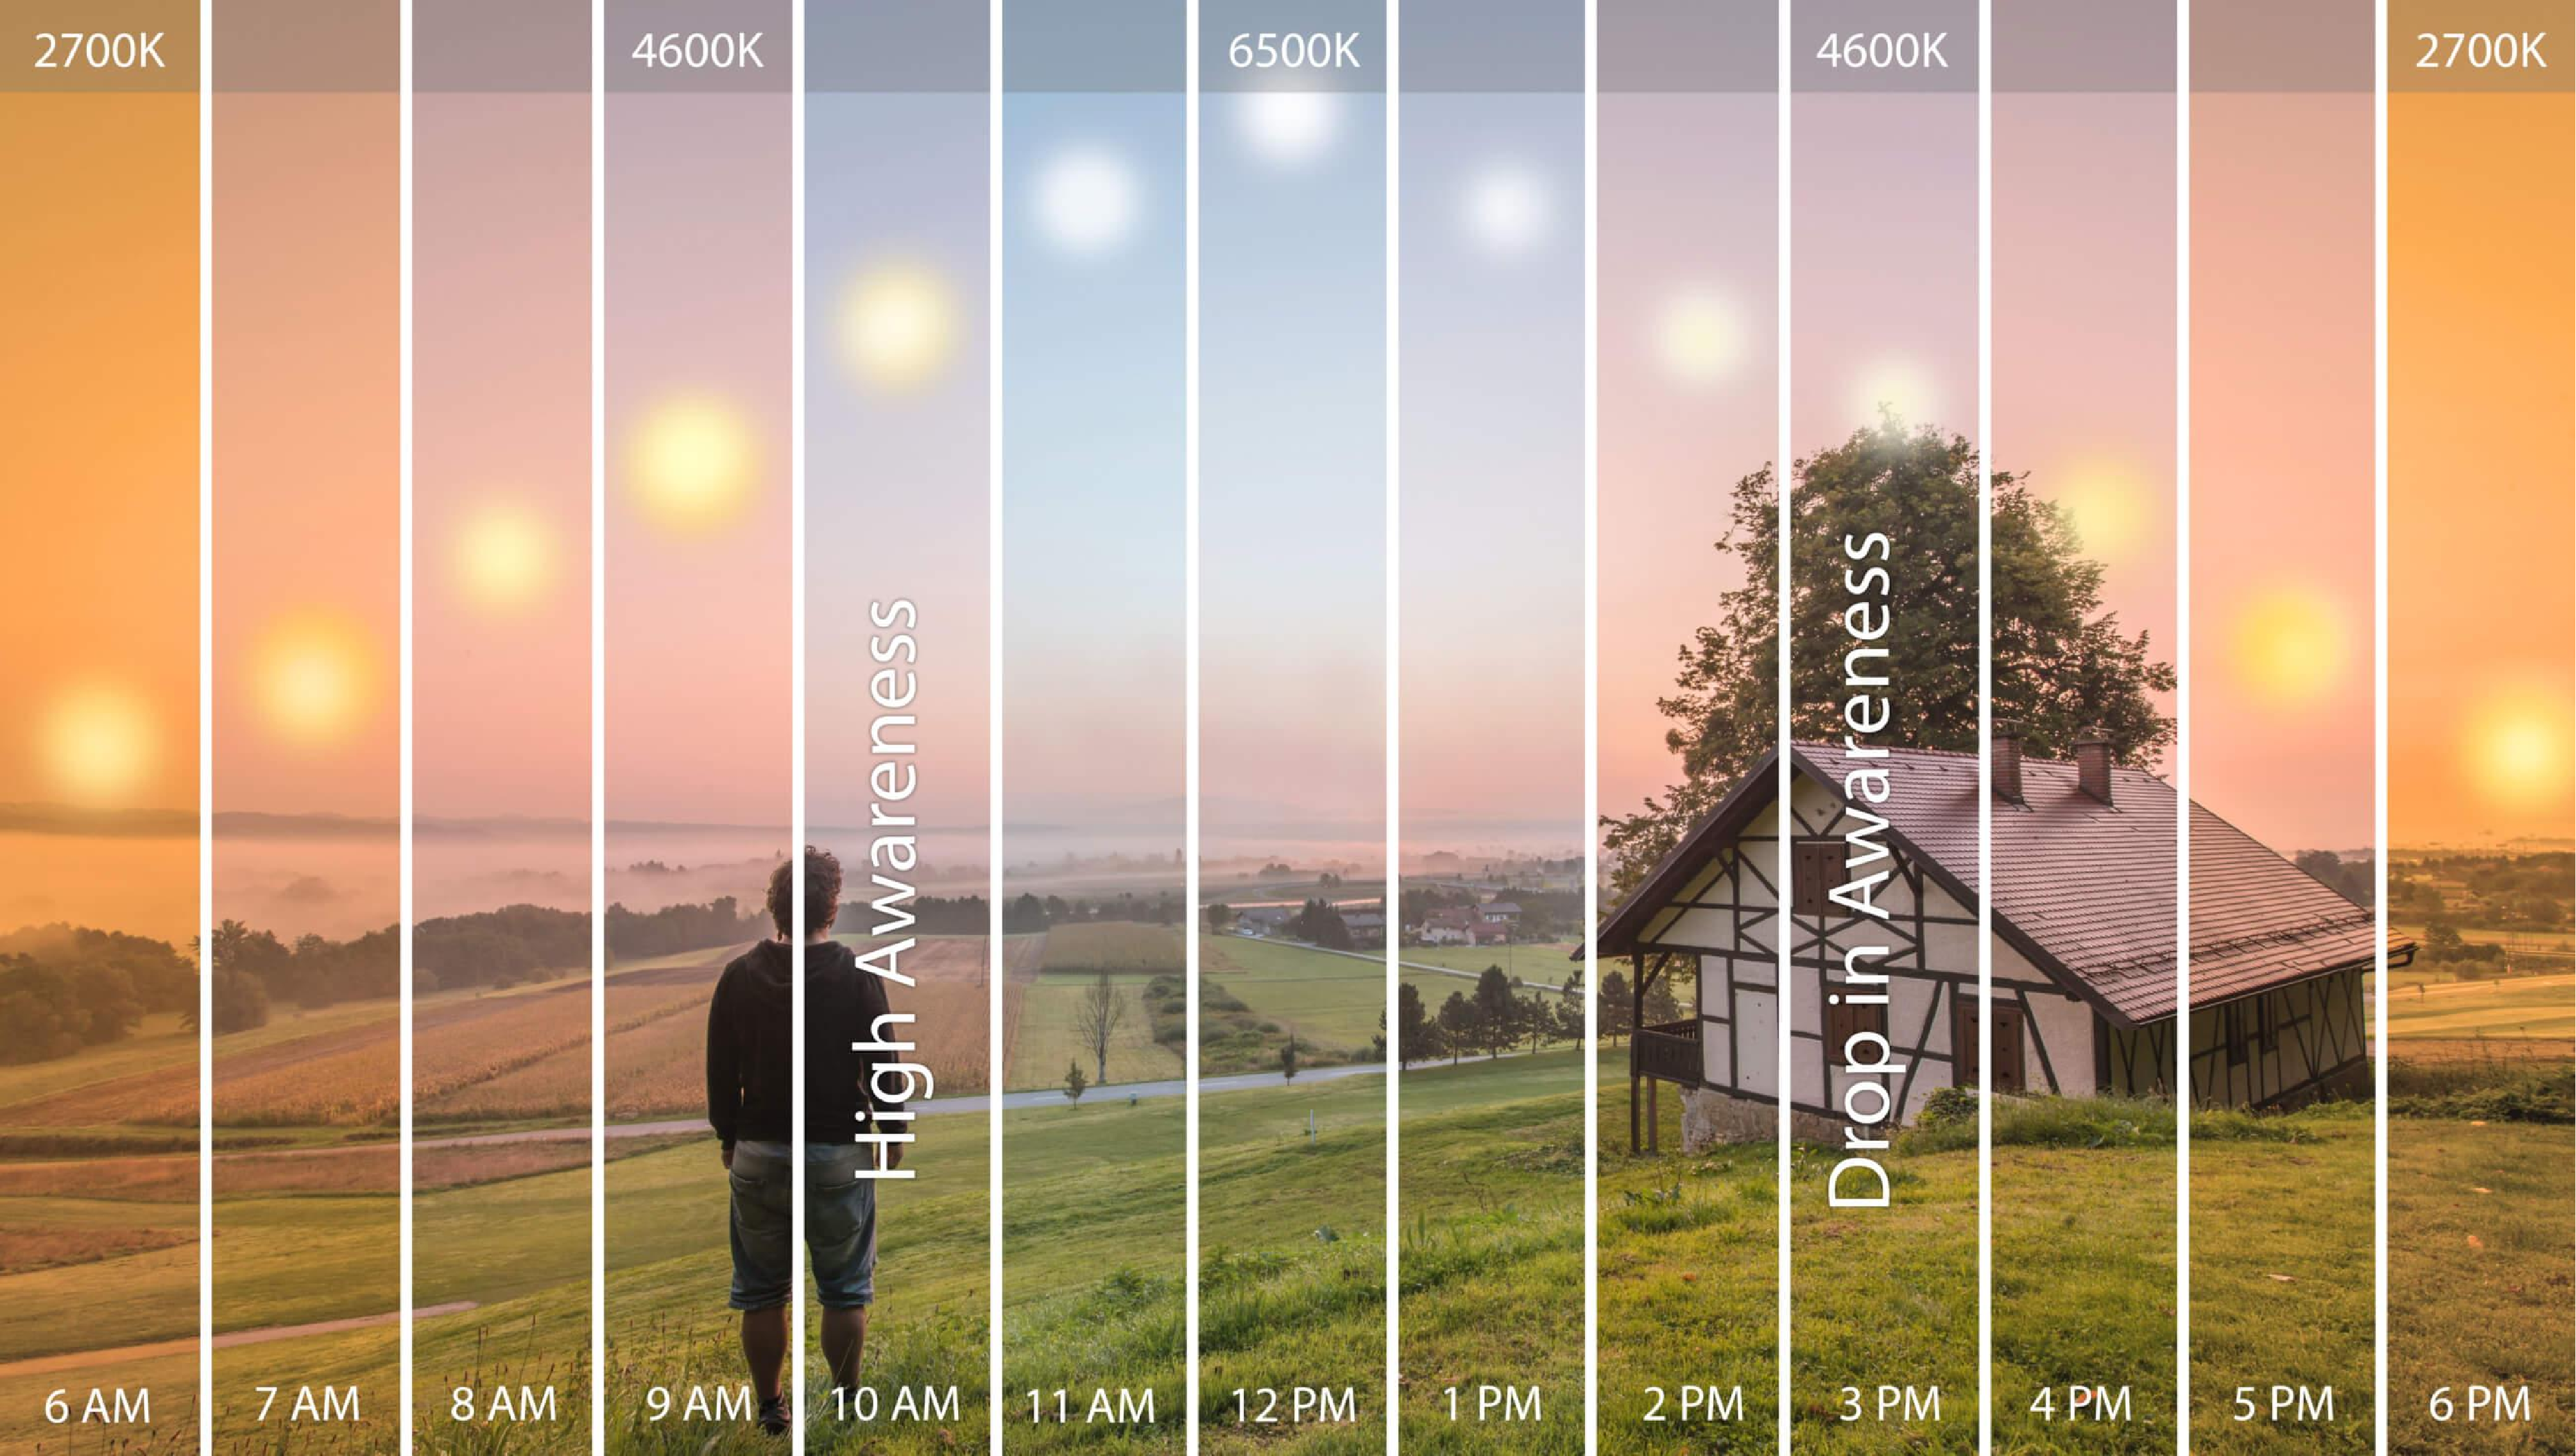
\includegraphics[width=0.8\linewidth]{docs/fig-chap1/fig-1-sunlight.pdf}
	\end{center}
	\caption{一天内太阳光色度的变化(图片来源于The Lighting Practice)}
	\label{fig:sunlight}
\end{figure}

% 高光谱成像是结合了光学成像和光谱学的优点、可以从场景中同时采集空间和光谱信息的一种新兴技术\cite{cao2021hyperspectral}。
与仅包含红绿蓝三个谱段(Red, Green, Blue)的 RGB 图像相比,HSI包含数百个谱段,跨越电磁波谱的紫外、可见光、近红外、中波甚至长波红外区域。一幅HSI相当于数百幅灰度图像,不仅记录了场景中物体丰富的空间结构,同时图像中每一个像元都对应一条与场景中物体材质相关的光谱曲线,使得HSI能够检测和分析不同物质间细微的光谱特征差异。因此,HSI广泛应用于现实世界的各个方面,成为环境、农业、地质和矿产勘探、生物、医学和军事侦查等\cite{teke2013short-app,lu2014medical-app,adao2017hyperspectral-app,khan2018modern-app,lu2020recent-app}领域研究的有效技术手段,发挥着越来越重要的作用。

% “同物易谱”、“异物同谱”一直是制约高光谱图像识别与理解性能的一大核心难题。
% 究其根本原因是由于
光谱成像过程受到成像机理、大气条件、环境光照等因素的影响,导致HSI的光谱信息、环境光照及其他信息相互耦合\cite{李树涛2023高光谱遥感图像本征信息分解前沿与挑战}。因此,有必要研究影响光谱成像过程的各种因素,环境中的光源就是其中之一。

若拍摄场景的光源条件不可控,即光源光谱未经标定或测量,则需要从图像中估计未知的光源光谱,该任务被称为光源光谱估计。关于高光谱成像技术中的光源估计问题目前研究尚少,相关解决方案仍未被深入探索\cite{鲁洋2022基于单幅多光谱图像的照明光谱估计方法}。为进一步推进高光谱领域的深度学习算法研究,有必要简化光源光谱测量流程或尽可能准确地估计光源光谱,保证光源条件不可控场景下的高光谱图像的有效性,从而高效地构建大规模高光谱图像数据集。

% 图像增强。
% 高光谱图像本征信息分解是高光谱遥感领域近年来出现的一项新兴技术。自文献[16]提出基于本征信息分解的高光谱图像特征提取方法以来,本征信息分解在高光谱遥感领域被赋予了新的内涵。与包含红、绿、蓝3个通道的彩色图像不同,高光谱图像是从可见光到红外数百个谱段图像构建的三维图像堆栈,既包含了丰富的空间结构也包含了精细的光谱信息。高光谱图像本征信息分解不仅仅是将输入图像分解为光照与颜色,同样也是将图像分解为与物体几何特性相关的空间光照图及与物体材质直接相关的光谱反射率图。
% 高光谱图像本征信息分解是高光谱研究领域近年来出现的一项新兴技术。% 自Kang等人\cite{kang2014intrinsic}提出基于本征信息分解的高光谱图像特征提取方法以来,本征信息分解在高光谱领域被赋予了新的内涵。
排除影响光谱成像过程的各种因素后,高光谱图像中的每一个像元就对应于该位置的物质的光谱本征信息。

高光谱图像本征信息分解不仅仅是将输入图像分解为光照与颜色,同样也是将图像分解为与物体几何特性相关的空间光照图,以及与物体材质直接相关的光谱反射率图,分别对应于图像增强任务及材质分割任务。然而,现有的高光谱图像本征分解工作大多专注于提出一些高光谱本征分解框架,最后在公共数据集上验证该本征分解方法的性能优劣,没有将分解后得到的本征图像进一步推广至现实场景应用\cite{李树涛2023高光谱遥感图像本征信息分解前沿与挑战}。一些研究者已经证实,相比于高光谱原始图像,高光谱本征图像在矿物勘探、变化检测领域都为解译模型带来了性能上的提升,但在军事侦察等其他领域暂时还未出现高光谱本征图像的成熟应用先例\cite{gao2021multitemporal, duan2020component}。为进一步促成科研成果的高效转化落地,有必要围绕下游应用开展高光谱图像本征信息分解研究,贴合实际场景对本征分解方法进行适应性改进,从而较大限度地发挥高光谱图像本征信息分解方法的潜能。

综上所述,本文重点研究从高光谱图像中估计光源光谱与分解光谱图像的关键技术,以提高光源估计的准确度,并将分解的光谱图像用于下游任务。本文的研究成果将对大规模高光谱图像数据集的构建和高光谱图像本征信息分解的应用提供方法借鉴。估计并校正光源光谱,能够尽可能地保证光源条件不可控场景下的高光谱图像有效性,提高高光谱图像数据集构建的效率。作为高光谱图像本征信息分解的输出,空间光照图能够用于引导图像进行亮度调整;同时,光谱反射率图能够用于辅助图像进行材质分割。

% 环境中的光源光谱可以通过捕获的光谱图像倒推得到,
% HSI中每个像素可以被视为包含特定波长下材料光谱反射率的向量

% 尽管现有的基于HSI的分类、检测和分割方法已经取得了显着的成效\cite{ahmad2021hyperspectral, su2021hyperspectral,huang2021weakly},但大多数方法都忽略了场景光源条件的影响。
% 在不同的室内光源下,在不同季节或昼夜的太阳光照下,如图\ref{fig:sunlight},相机捕获到的图像的整体颜色有很大差异。这一问题在RGB图像领域常作为颜色恒常问题\cite{gijsenij2011computational,RN30,RN14,RN13,RN9,RN8}进行研究。专业摄影时,往往使用标准色卡来校正光源、镜头、传感器等多方面因素带来的差异。

% 通常,可以在场景中放置白板来捕获光源条件,但仅适用于静态场景和空间一致性光源。

% 计算成像的进步\cite{dai2014computational}促进了高光谱图像的获取,导致高光谱图像数据集显着扩展。但经过良好校正的高光谱图像数据集很少见。根据校准方法不同,高光谱图像数据集可以分为三种:

% (1)复杂校准:这种数据集涉及复杂的校准流程\cite{guanter2006spectral},包括大气反射校准,通常应用于遥感卫星数据。这些数据集中的图像数量较少,甚至只有一张,例如 Indian Pines、Pavia University 和 Salinas 数据集。

% (2)基于光源的校准:这种数据集通过漫反射板或专门的测量设备获取光源信息来校准\cite{alvarez2016practical},但是无法准确校准复杂光源。此类别的数据集通常具有中等大小\cite{li2021multispectral}。

% (3)无校准:这种数据集不包含任何形式校准\cite{arad2020ntire,arad2022ntire}。这些数据集的大小往往较大。

% 光谱图像标定大致可以分为两部分:光谱标定\cite{guanter2006spectral}和几何标定\cite{kim2015geometrical}。这里只讨论受光源影响的光谱标定。

% 如图\ref{fig:ntire}所示,一些高光谱图像数据集\cite{arad2022ntire}中的图像并没有包含白板,这时就需要从高光谱图像直接预测光源光谱。

% 无论是直接测量还是通过各种方法预测,场景的光源信息对于后续视觉任务都有重要作用,包括图像增强这样的低层级(low-level)任务和语义分割这样的高层级(high-level)任务。

% 对于图像增强这样的任务,高光谱数据
% 然而,一些 HSI 数据集不捕获白板或测量光源。因此,提出了一种称为高光谱光源估计的任务,旨在从获取的高光谱图像中推导出光源光谱。

% 我们提出了一种端到端网络来解决高光谱光源估计问题。与现有的基于学习的方法相比,我们的方法使用了更深的主干网络resnet50,这显着提高了使用CNN进行光源估计的性能。此外,我们针对高光谱光源的特点引入了通道和空间自注意以及平滑损失,以进一步提高估计的准确性。

% 高光谱光源估计的研究很少,并且缺乏专门为此任务设计的数据集。我们构建了一个具有切换光源的真实高光谱图像的大型数据集 HSISI。该数据集中的每个场景都包含多种光源的数据对,为系统研究高光谱光源估计提供了素材。

% 与RGB图像相比,高光谱图像具有高维优势。我们相信高光谱图像可以更好地描述光源光谱,从而更准确地预测光源光谱。颜色恒常性问题首先需要估计场景中的光源,然后对图像进行校正。
\section{国内外研究现状及存在的问题}
\subsection{国内外研究现状}
% \leftline{}
\textbf{1.光源光谱估计研究现状}
% 与高光谱图像光源估计问题相近的问题是颜色稳定性问题,在颜色稳定性问题的研究中,往往需要先进行光源估计。% \subsection{基于统计的方法}

高光谱图像可以分解为光源光谱和反射率光谱,光源光谱估计则专注于从高光谱图像中提取光源光谱。

光源光谱估计方法可以大致分为两类: 基于统计的方法和基于学习的方法。在深度学习普及之前,人们通过统计图像中的像素点来估计光源光谱;随着深度学习算法的开发和算力的提高,人们更倾向于训练模型来预测光源光谱。

首先是基于统计的方法,这类方法是基于捕获场景的统计特性并利用这些先验提供的假设来估计光谱。最开始的光源光谱估计方法受RGB图像的光源估计启发,一些经典方法假设光源颜色可以直接通过以下方式获得:图像中所有像素颜色的均值(Gray-World)\cite{RN6} ,或具有最大光谱响应的像素(Max-RGB)\cite {RN19},或图像中主要目标的边缘像素(Gray-Edge)\cite{RN30}。这些假设适用于颜色恒常性问题\cite{gijsenij2011computational,RN30,RN14,RN13,RN9,RN8},也适用于光谱的光源估计任务并表现良好\cite{RN17,RN18}。通过这些假设,可以估计出光源每个波长通道的光谱功率分布(Spectral Power Distribution, SPD)。此外,Khan等人\cite{RN16}和Su等人\cite{RN28}}分别提出,从多光谱或高光谱图像中捕获的镜面反射可以提供有关场景光源的信息,但这些方法依赖于非朗伯表面来提取镜面反射分量,不适用于仅含有朗伯表面的场景。Zheng等人\cite{RN35}提出了另一类方法,通过利用光谱反射率的低秩特性来分离光源光谱和反射率。然而,在更一般的场景中,仅仅依靠单一假设来实现准确的光源光谱估计往往是不够的,许多基于统计的方法都是对所有场景使用同一组固定的超参数,使得估计的准确性对超参数设定和成像条件高度敏感。
% RN17,RN18,RN16,RN28,RN35
% \subsection{基于学习的方法}RN24,li2021multispectral

然后是基于学习的方法,一开始,深度学习技术被用于对RGB图像中的光源颜色进行估计\cite{dsnet,RN13,RN1,RN31},这些方法利用大规模图像数据集,相比基于统计的方法具有更高的精度。后续的研究将基于学习的模型扩展到高光谱领域,Robles等人\cite{RN24}利用卷积神经网络(Convolutional Neural Networks, CNN)来估计光源光谱,为了获取图像整体和局部光源信息,采用多尺度输入作为前端网络。Li等人\cite{li2021multispectral}将光源估计作为一个矩阵分解问题求解,并采用深度展开网络来优化矩阵分解,将高光谱图像分解为光源和反射率。

% 基于学习的方法比基于统计的方法得到的光源估计结果更加准确,但是目前现有高光谱光源估计数据集的数量增加速度缓慢,。
% 然而,由于高光谱的通道数远高于RGB的通道数,Alexnet\cite{RN24}等浅层神经网络很难提取高光谱的高维特征。

% 一般来说,基于学习的方法比基于统计学的方法得到的结果更加准确。这些研究中考虑的特征大多是手工制作的,包括色度直方图\cite{RN21,RN23,RN24}、完整的三维RGB直方图\cite{RN9,RN25}、以及频域特征。最近的方法表明,相对简单的特征,如颜色和边缘矩\cite{RN26},或颜色色度\cite{RN28}的统计,可以提供良好的性能。虽然CNN学习的深度表征在各种高层级任务和一些低层级视觉问题中取得了显著的成功,但深度CNN是否能在颜色稳定任务上表现良好尚不清楚。在图像中光谱分布均匀的假设在某些常见情况下,有多个光源或阴影内加非阴影区域的场景中可能不起作用。

% (1)基于统计的方法,基于图像统计或物理性质来估计光源。这些方法考虑了颜色统计和消色差颜色\cite{RN6,RN7}之间的关系,来自人类视觉系统\cite{RN8,RN9,RN10}的统计,来自图像和场景光源\cite{RN13,RN14}的空间导数和频率信息,以及窥镜和阴影\cite{RN16,RN17,RN18};(2)基于学习的方法,使用从训练图像中学习的模型来估计光源。

% 延伸到高光谱图像的光源估计,一个实际的解决方案是从捕获的多光谱图像中估计光源光谱,并进一步分离反射率和光源光谱。这个光源估计问题是高度欠确定的;因此,需要正则化来约束解,以满足多光谱重反射和光源的图像先验。近年来,人们研究了许多估计光源光谱的方法。大多数要么利用多光谱图像的统计,要么提取镜面反射分量来估计合成光谱。也有使用卷积神经网络\cite{RN24}或者深度展开网络\cite{li2021multispectral}进行高光谱光源估计的研究。

\textbf{2.光源光谱引导的图像增强研究现状}

图像增强的目的是改善被掩盖的图像细节,突出图像中有用的信息和感兴趣的特征\cite{liu2022survey},图像增强的广泛研究为许多先进的研究领域做出了贡献\cite{IE3},例如大气科学、天文学、海洋学、遥感成像、医学成像等。

图像增强任务包含的研究范围很广,对于不同的图像增强目的则对应着不同的方法。Dileep和Murthy\cite{IE14}为了消除图像中存在的照明效应,使用Retinex算法和同态滤波(Homomorphic Filter)算法,实现了低对比度图像的色彩渲染和动态范围压缩。

更多与光源相关的图像增强工作聚焦于图像色彩校正方法。Ancuti等人\cite{IE108}提出了一种无监督的全局和局部色彩增强方法,考虑图像中的颜色空间分布,提取具有不同光照条件的图像中的视觉信息,结果表明该方法在颜色恒常校正和色调平衡方面具有良好的性能。Shi等人\cite{IE111}使用归一化伽玛变换和对比度限制的自适应直方图均衡(Adaptive Histgram Equalization, AHE)来校正图像颜色失真,在此方法中,输入的 RGB 图像首先转换为$Lab$色彩空间,将归一化伽马校正算法应用于增强图像$L$分量的对比度,使用基于灰色世界的颜色校正函数增强$a$和$b$分量,由于使用了$Lab$色彩空间,增强后的图像没有颜色偏差。Afifi等人\cite{IE112}提出的方法将色偏向量(Color Cast Vector)与颜色校正函数连接起来,通过现成的照度估计函数来估计色偏向量,对每个色偏向量进行聚类,采用最合适的聚类对应的颜色校正函数来生成颜色校正图像。Tai等人\cite{IE106}提出的方法应用了两种常用的颜色增强假设:灰色世界和颜色直方图拉伸函数的宽色域特性,可以很好地保持色彩对比度,避免过度拉伸问题,能够保留原始图像的自然度,尤其适用于色彩失真明显的图像。

% Buades等人\cite{IE15}回顾了不同的图像去噪算法(例如高斯平滑、各向异性滤波、全变分细化、SUSAN滤波器、维纳局部经验滤波器、平移不变小波阈值处理、离散通用降噪器、无监督信息论自适应滤波和非局部均值)和 然后提出了一种新方法来避免产生伪影或去除图像精细结构。 他们还将所提出的方法与其他经典图像去噪算法进行了比较。 Motwani 等人的类似论文。 [16]介绍了图像去噪领域中几种常用的图像增强方法(例如数据自适应阈值、未抽取小波变换、独立分量分析等)。 

\textbf{3.光源光谱校正的材质分割研究现状}

材质分割是对图像中的材质进行像素级的识别\cite{liang2022multimodal},与语义分割相似,但是可能需要将同一语义进一步分为不同的材质,例如将树分为树干和树叶。

材质分割数据集为材质分割的研究提供了数据基础。Dana等人\cite{MS5}构建了一个在205个光源种类及其方向组合中拍摄的61个不同纹理样本的数据集,每张图像仅包含一种材质,用于研究光源种类和光源方向对材质的纹理特征的影响。Bell等人\cite{MS1}构建了一个包含23种材质的200万个64×64分辨率图像块的数据集,基于CNN和条件随机场(Conditional Random Field,CRF),将大量的样本用于材质分割模型的训练。Schwartz和Nishino\cite{MS21}在PASCAL VOC\cite{VOC},MS COCO\cite{COCO}和ImageNet\cite{IMAGENET}三个大规模数据集的基础上进行材质分割的标注,引入了一种深度网络架构,整合了局部材质特征和全局语义信息。Liang等人\cite{liang2022multimodal}构建了包含RGB图像、近红外图像和偏振图像的多模态材质分割数据集,并用语义分割的结果作为图像分区域学习的依据。

由于语义分割与材质分割的相似性,前者为后者的网络设计提供了思路。语义分割在引入了全卷积网络后,用卷积层代替全连接层,在分割精度上有了显著进步\cite{MS14}。Chen等人\cite{MS2}提出了动态区域感知卷积(Dynamic Region-Aware Convolution, DRConv),自动地将多个卷积核分配给特征表示相似的空间区域,在提升性能的同时,还维持了一定的空间不变性。Deeplabv2\cite{MS3}采用空洞空间卷积池化金字塔(Atrous Spatial Pyramid Pooling, ASPP)来提取多尺度特征。Deeplabv3+\cite{deeplabv3+}则采用编码器加解码器的结构,进一步提升了图像分割的精度。
% Yu等人\cite{MS28}介绍了扩张型骗局克服玉米玉米[28]有限的接受能力。
% \cite{MS30}解耦动态滤波器(DDF)分离了这些动态火焰的空间和通道成分,以降低计算成本。

\subsection{研究存在的问题}
根据现有的研究成果,可以发现以下几个方面的不足。

1、由于从单个图像中恢复像素级光源光谱是一个约束不足的问题,现有的方法通常假设整个场景具有均匀的光源分布。基于统计的光源估计方法通常假设场景具有特定的统计分布特征,例如光照的分布服从某种概率模型。然而,真实世界中的场景往往具有非常复杂的光照条件,这些假设可能无法完全捕捉到场景的真实特征,从而导致基于统计的方法的适用范围受到限制。

% 2、基于学习的光源估计方法使用的模型还停留在早期的计算机视觉模型,缺少Transformer、扩散模型等新的视觉模型的研究。同时,缺少真实高光谱的光源估计数据集,已有的数据集普遍使用仿真实现,难以验证在现实中的泛化性。

2、缺少将光源估计与各种视觉任务相结合的研究,已有的光源估计研究主要解决颜色稳定性问题,如色彩校正,白平衡等。在本征分解、重照明等任务中则将光源估计与其他要素相叠加,并没有单独考量光源估计的准确性。

\section{论文研究内容及章节安排}
本文围绕高光谱图像的光源光谱问题,基于深度学习理论,并结合自注意机制、损失函数设计、局域与全局分析、反射率分解等方法,从光源光谱的估计出发,以图像增强和材质分割为例,探索光源光谱在低层次问题和高层次问题的应用。

% 本文围绕高光谱图像的光源光谱估计问题及其应用展开研究。首先预测高光谱图像的光源光谱,然后使用光源光谱引导RGB图像的动态范围压缩,最后使用光源光谱对RGB图像进行校正并用于材质分割。主要工作和创新点包括以下几个方面:

% 1、光源光谱估计。构建了真实而非仿真的高光谱光源估计数据集;提出了光谱联合空间自注意机制,用于突出重要的光谱通道和图像中有效区域的作用;提出了平滑约束的损失函数,避免了不实际的病态结果,从而提升了光源估计的准确度。

% 2、光源光谱引导的动态范围压缩。构建了RGB图像与高光谱图像对齐的动态范围压缩数据集;提出了局部亮度适应法,调节高动态范围RGB图像不同区域的亮度;提出了光谱感知自注意机制,将光源光谱嵌入到RGB特征图中,提升了RGB图像动态范围压缩的效果。

% 3、光源光谱校正的材质分割。构建了RGB图像与高光谱图像对齐的材质分割数据集;提出了光谱联合RGB分解模型,使用光源光谱校正RGB图像的反射率,有效提高了RGB图像的材质分割精度。
\begin{figure}[h]
	\begin{center}
		%\fbox{\rule{0pt}{2in} \rule{0.9\linewidth}{0pt}}
		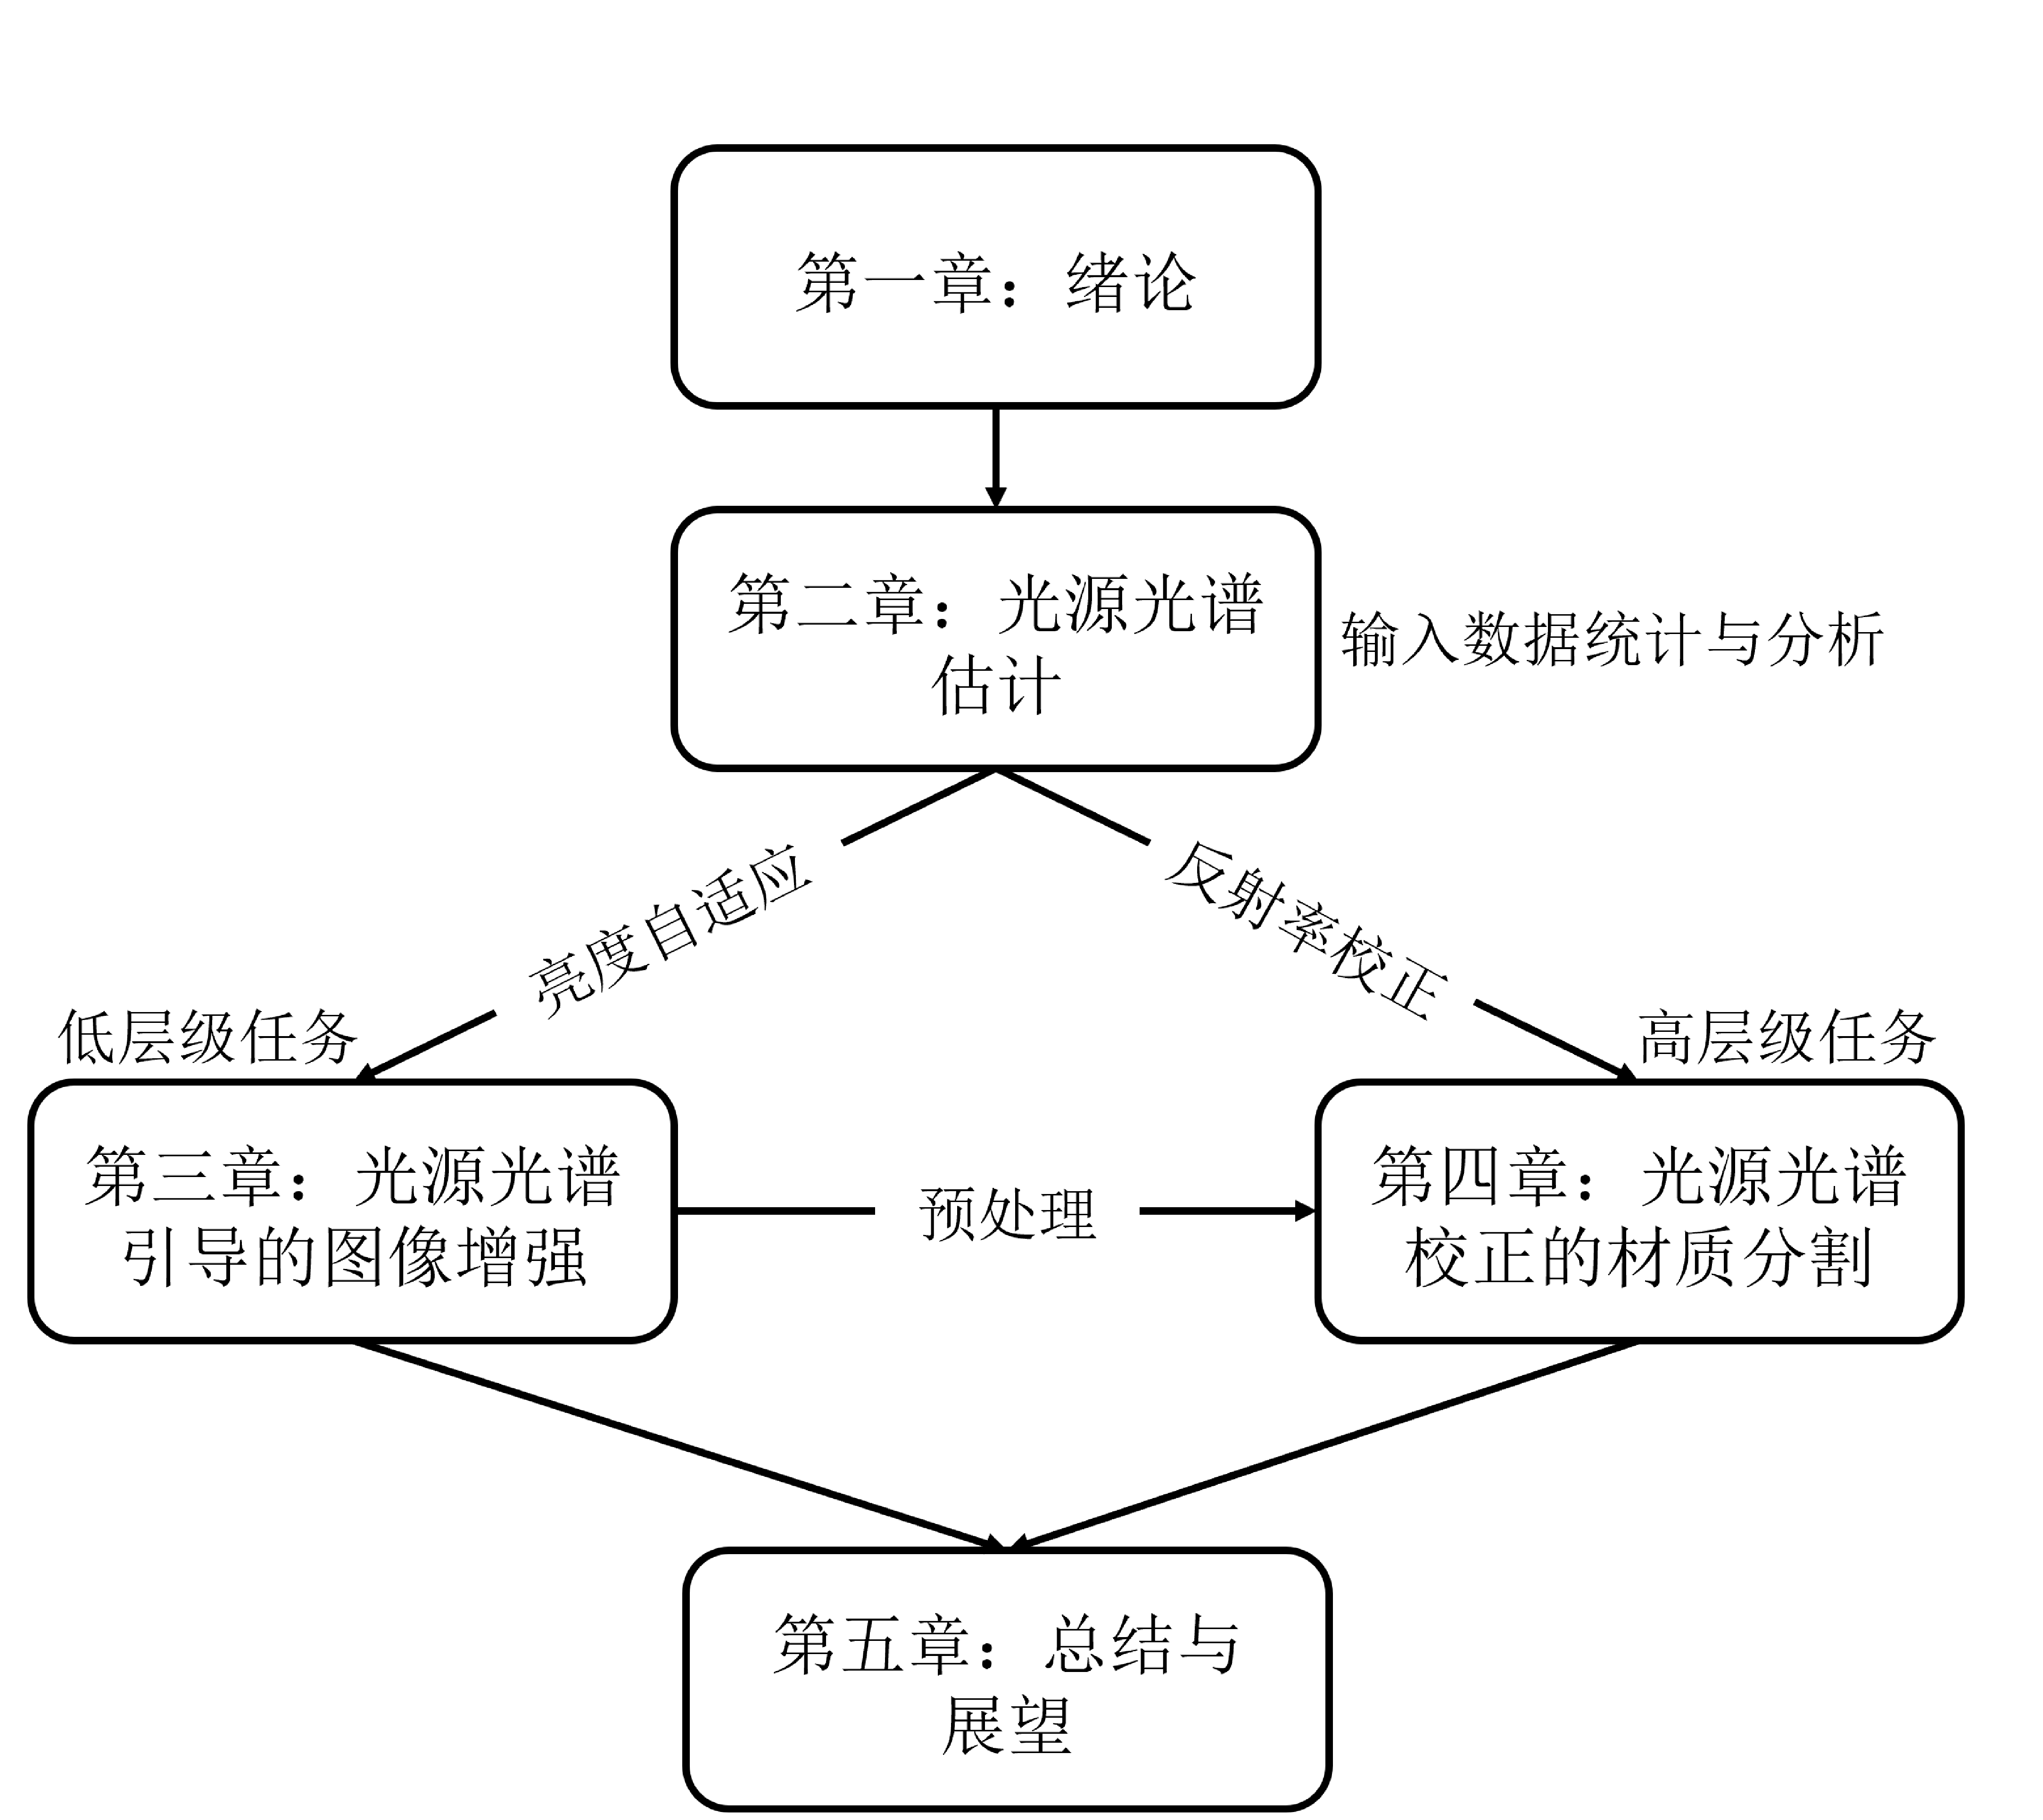
\includegraphics[width=1.0\linewidth]{docs/fig-chap1/fig-1-structure.pdf}
	\end{center}
	\caption{论文组织结构图}
	\label{fig:structure}
\end{figure}

本文的组织结构如图\ref{fig:structure}所示。

论文章节安排具体内容如下:

第一章,绪论。主要介绍了高光谱图像中光源光谱的重要性、研究现状以及目前光源光谱研究的发展趋势和存在的不足。最后给出了本文研究内容的框架和章节的分布及每章的贡献介绍。  

第二章,光源光谱估计。利用深度学习的方法对高光谱图像进行光源光谱估计,构建仿真数据集并拍摄真实数据集,提出了光谱联合空间自注意机制以及基于光源特性的损失函数。

第三章,光源光谱引导的图像增强。利用第二章估计的光源光谱结果来引导RGB图像的高动态范围增强,拍摄并构建了高光谱与RGB对齐数据集,提出了局部亮度适应法和光谱感知自注意机制。

第四章,光源光谱校正的材质分割。利用第二章估计的光源光谱结果来校正反射率,并利用第三章的图像增强方法对RGB图像进行预处理,在第三章的数据集的基础上进行材质分割标注,以构建高光谱-RGB材质分割数据集,提出了光谱联合RGB分解模型。

第五章,总结与展望。对本文的研究内容及研究结论加以归纳总结;阐述本论文研究内容的欠缺之处,并对下一步的研究内容及方向做出展望。 

%---------------------------------------------------------------------
%	第二章
%---------------------------------------------------------------------
\chapter{光源光谱估计}

\section{引言}
% 对于RGB图像,已有不少的光源估计的工作,但是对于高光谱图像则鲜有研究。可以借鉴RGB图像的光源估计方法,适配到高光谱图像。

% 在相关摄影摄像拍摄过程中不同的颜色的光源对拍摄对象拍摄后所反映的被实体的照片或影像的颜色有严重的真实反馈的影响,例如我们用红色造测白色的物体,白色物体在rgb图像中反映出的大部分色彩就是红色的了,而用蓝色光源照射黄色物体说拍摄出来的图像的颜色为为黑色,那么如此,颜色的混合会导致对摄物体反馈的颜色就和它的物体的本身颜色不同,在工程或者科技应用当中会产生混淆紊乱的图像辨别问题,如果引入一种光源光谱估计的算法,将光谱的本真波段或者是什么东西,嗯,辅助加入岛,照射光源的同步同步引入到照射光源的这个对物体进行照射与拍摄,能够通过光源光谱估计的相关算法,能够得出来。被拍摄了物体的表面的的真实颜色本身,这就是光源光谱估计研究的目的。高光谱具有不同的这个多维通道。这个通道,能够全面的覆盖RGB
关于高光谱成像技术中的光源估计目前研究尚少,相关解决方案仍未被深入探索\cite{鲁洋2022基于单幅多光谱图像的照明光谱估计方法}。若光源光谱无法估计,则高光谱图像的光谱反射率重构将面临巨大挑战。

光照的变化对高光谱技术的实际应用也是一项艰巨的挑战\cite{曹汛2020计算光谱成像的前沿进展},为此,高光谱图像通常需要使用已知的色卡或白板作为参考\cite{li2021multispectral}或使用专用测量设备\cite{alvarez2016practical}进行校准,以确保光谱反射率的测量准确且一致。

\begin{figure}[h]
	\begin{center}
		%\fbox{\rule{0pt}{2in} \rule{0.9\linewidth}{0pt}}
		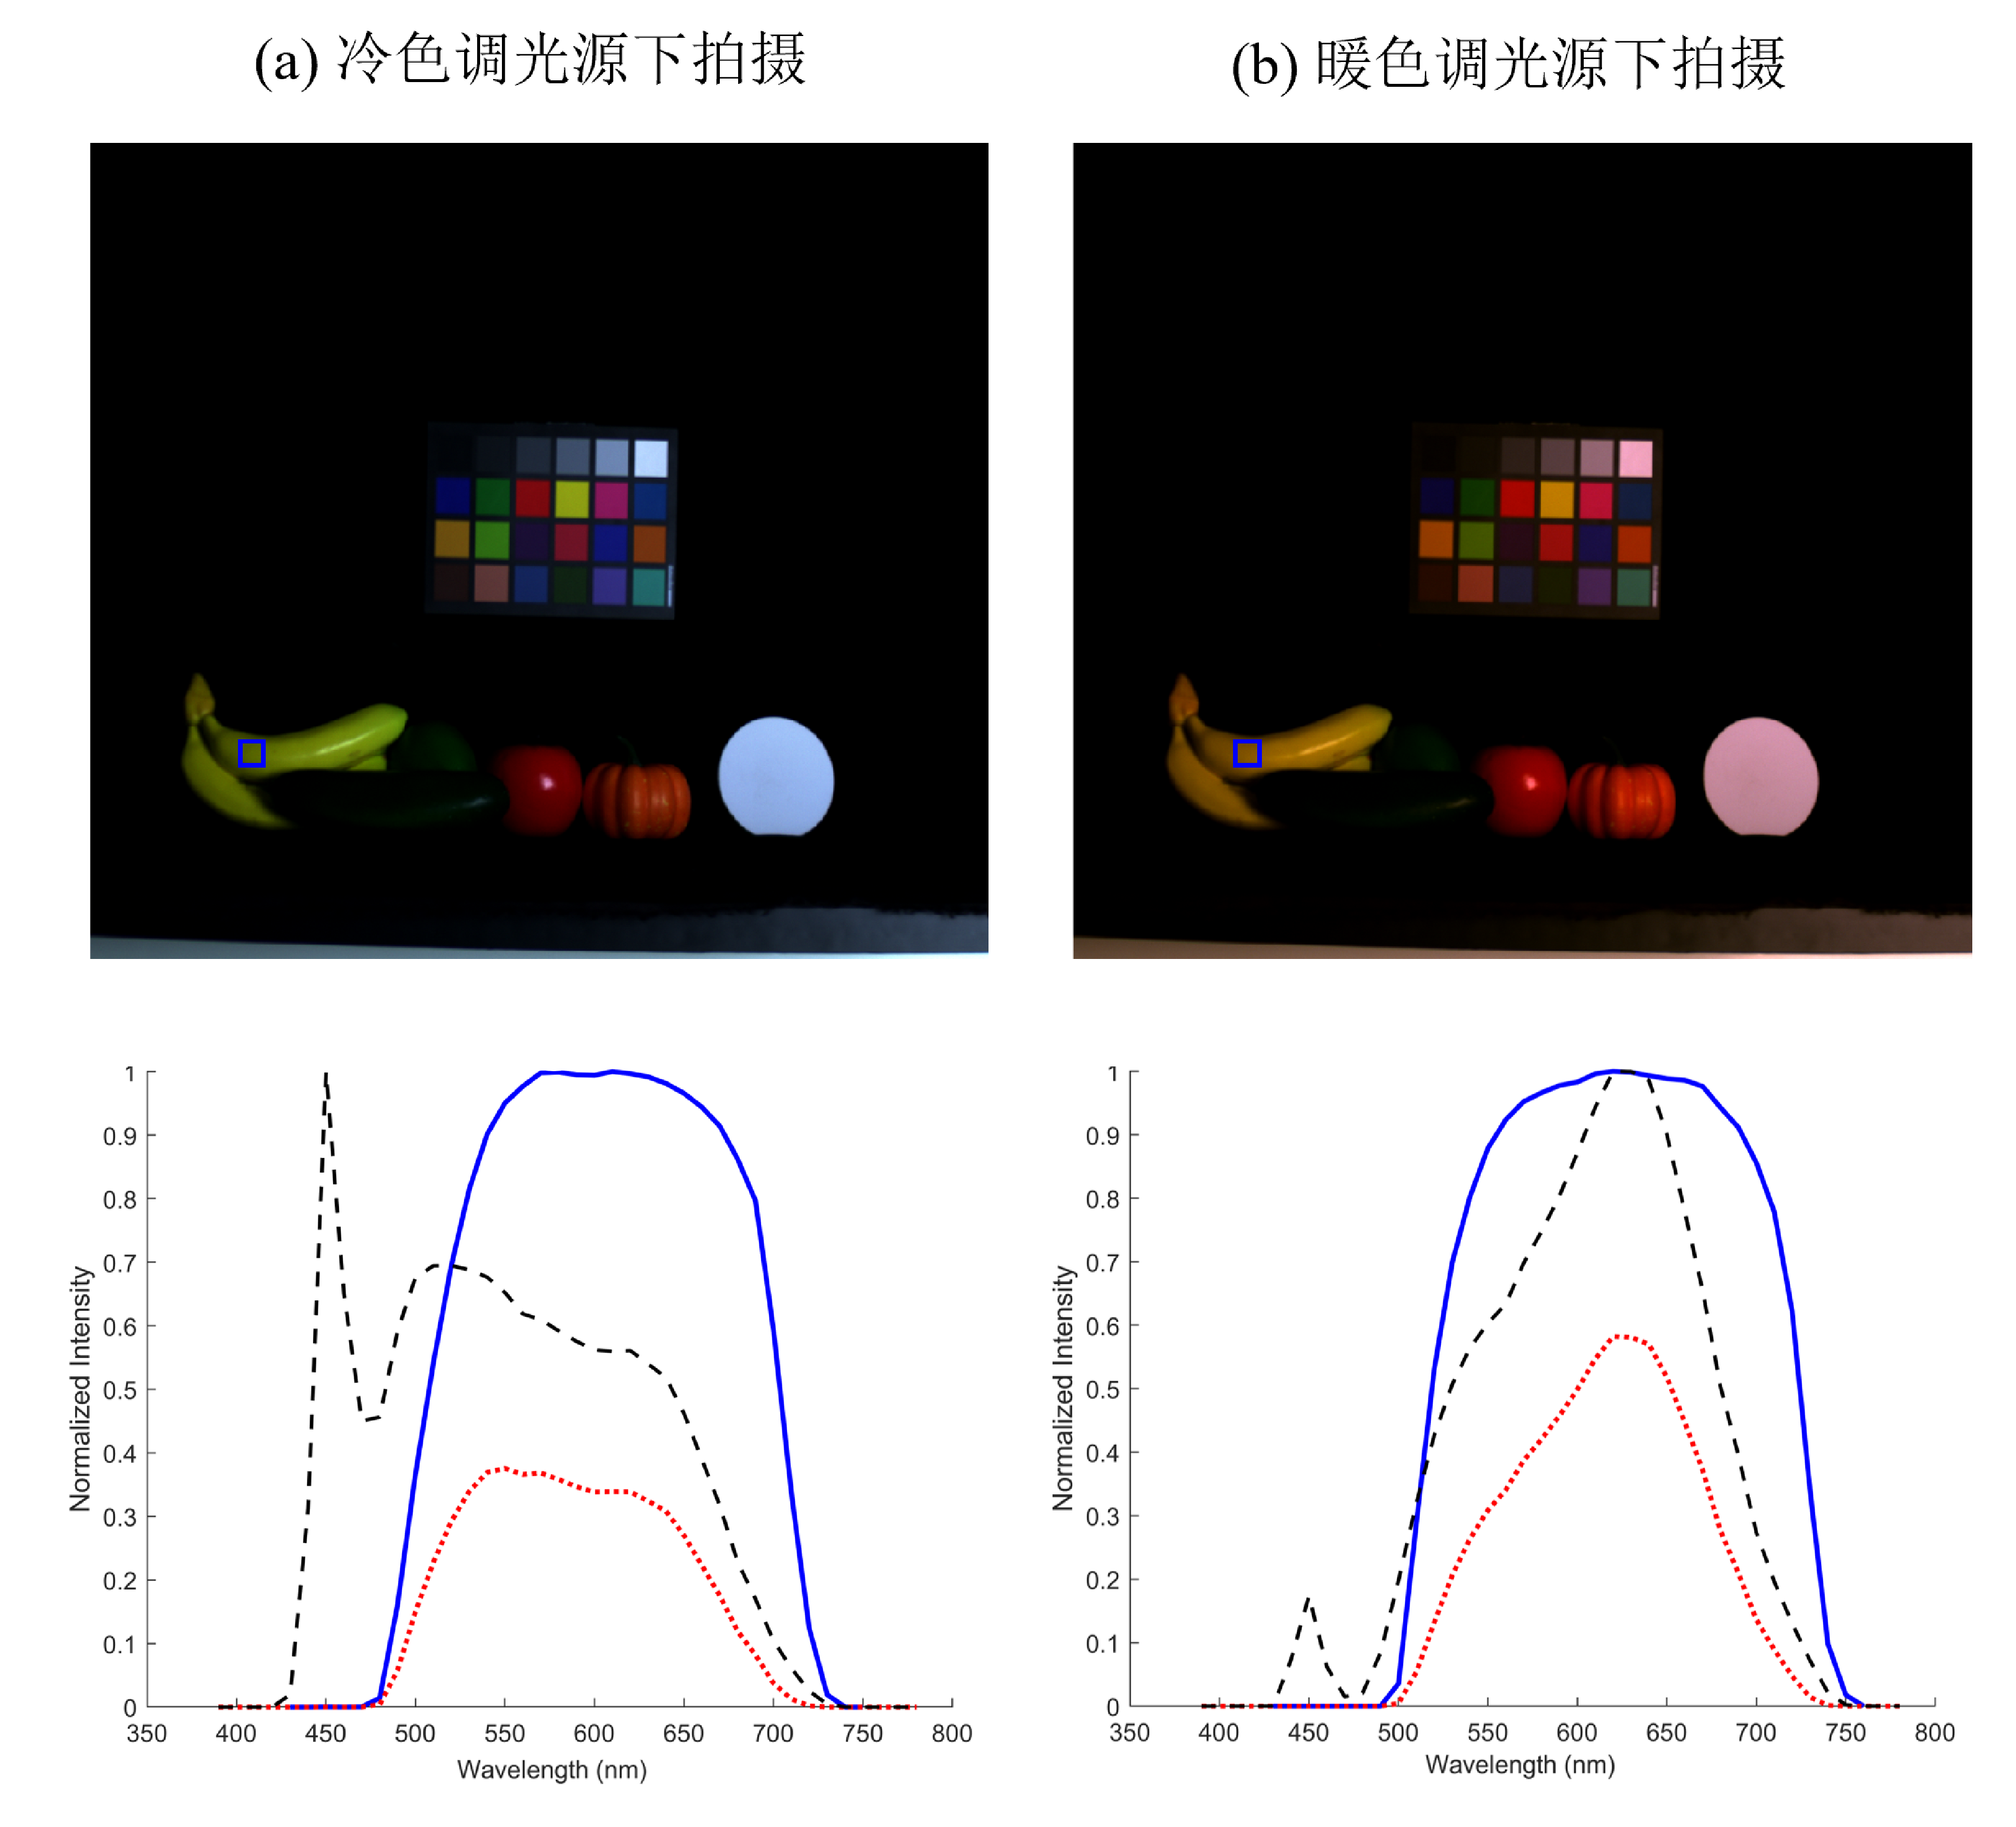
\includegraphics[width=0.8\linewidth]{docs/fig-chap1/fig-1-intro.pdf}
	\end{center}
	\caption{一些塑料水果模型在冷色调和暖色调光下的图像,相关色温分别为(a)6500K和(b)2500K,以及从蓝框区域反射的相应光谱,黑色虚线代表从白板获得的(归一化)光源光谱,红色虚线代表方框区域的测量光谱,蓝色线代表其校正的(归一化)反射率}
	\label{fig:correct}
\end{figure}
% 图 \ref{fig:correct} 显示了不同光源对测量光谱的影响的示例:用冷色调或暖色调光源的香蕉,以及如何校正光谱。物体的反射率保持不变,但在不同光源下的反射光谱有所不同。

如图 \ref{fig:correct} 所示,同一个物体在不同的光源下呈现出不同的光谱曲线,红色曲线代表的测量值明显与黑色虚线代表的光源光谱曲线具有形态上的相似性,体现出类似的能量分布,渲染为RGB图像则表现为场景中的物体与光源颜色相和谐。然而同样是香蕉的光谱测量值表现出不同:在冷色调光源下的测量值呈现出500nm和640nm两处较小的峰,而在暖色调光源下的测量值呈现出630nm一处较强的峰。将光谱测量值逐波段除以光源光谱再进行归一化处理,就得到了对应的反射率,这是物质的本征属性,是可以用于区分物质的“基因”。如图\ref{fig:correct}中蓝线所示,不同光源下香蕉的光谱曲线在校正后变得一致。

上述的校准方法假设场景具有全局一致的光源光谱,在实际场景中,光源光谱的强度和光谱曲线可能随着空间位置而改变。

对于非全局一致的光源光谱估计,定义高光谱图像矩阵为 $\mathbf{I} \in \mathbb{R}^{H \times W \times C}$,其反射率矩阵为 $\mathbf{R} \in \mathbb{R}^{H \times W \times C}$,其中$H$是高度,$W$是宽度,$C$是通道数。 光源光谱矩阵为$\mathbf{L} \in \mathbb{R}^{H \times W \times C}$,满足 $\mathbf{I} = \mathbf{R}\odot\mathbf{L}$,其中$\odot$表示哈达玛积。对于全局一致的光源光谱估计,光源光谱退化为向量$L \in \mathbb{R}^{H \times W \times C}$,满足$\mathbf{I} = \mathbf{R}\cdot L$,其中$\cdot$表示点积。由此可知,无论是否假设场景具有全局一致的光源光谱,从高光谱图像中估计出光源光谱都是一个病态问题。
% RN17,RN18,RN16,RN28,RN35
% \subsection{基于学习的方法}RN24,li2021multispectral

具体来说,光源光谱估计方法主要分为两类:基于统计的方法\cite{RN17,RN18,RN16,RN28,RN35}和基于学习的方法\cite{RN24,li2021multispectral}。在基于统计的方法中,镜面反射分解\cite{RN35}针对场景中的非朗伯表面,从镜面反射中提取高光谱图像的光源光谱。在基于学习的方法中,深度展开网络\cite{li2021multispectral}将光源估计作为一个约束矩阵分解问题求解,并采用深度展开网络来优化矩阵分解,将高光谱图像分解为光源光谱和反射率。

近年来,基于Transformer的网络也被用于光谱相关的研究并取得了良好的效果\cite{cai2022mask,roy2023spectral,li2023spectral},得益于其全局感知能力,可以应用于全局光源光谱估计。

在本章中,本文以Transformer网络为基础,提出了光谱联合空间自注意机制,通过分阶段处理的方式避免了高维数据的“维数灾难”,用于突出重要的光谱通道和图像中有效区域的作用;提出了平滑约束的损失函数,避免了不实际的病态结果,从而提升了光源估计的准确度。
% ,据我所了解,本文包含了第一次将Transformer应用于高光谱光源光谱估计的尝试。构建了真实而非仿真的高光谱光源估计数据集;提出了光谱联合空间自注意机制,用于突出重要的光谱通道和图像中有效区域的作用;提出了平滑约束的损失函数,避免了不实际的病态结果,从而提升了光源估计的准确度。
% 关于高光谱成像技术中的光源估计目前研究尚少,相关解决方案仍未被深入探索\cite{鲁洋2022基于单幅多光谱图像的照明光谱估计方法}。Joze\cite{NTNU70}等人,并将其用于提高图像分类的准确度。Agarwal\cite{NTNU72}等人
\section{相关研究}
\subsection{基于学习的光源估计}
随着机器学习的快速发展,多种机器学习算法,尤其是深度学习算法也被应用于光源估计。Cardei等人\cite{NTNU69}用一个多层的神经网络来学习图像的色度直方图和光源色度间的关系。Wang等人\cite{NTNU73}提出了一种基于支持向量回归的光源估计算法,并表明图像的导数比图像的原始像素值更有效。Bianco等人\cite{NTNU77}将图像分为小的图像块,使用卷积神经网络进行局部的光源估计。

除了直接将机器学习方法用于光源估计问题,将光源估计问题转化为其他问题也是一种思路。Barron\cite{NTNU71}将光源估计问题重新表述为一个在色度空间中的二维空间定位任务,从而将目标检测和结构化预测等技术应用于光源估计。Lou等人\cite{NTNU74}将光源估计问题看做回归问题,提出了使用深度神经网络进行光源估计的新框架。Shi等人\cite{NTNU75}提出的方法将光源估计作为两阶段的任务,首先用一个深度网络提出光源估计的多种可能,然后用另一个深度网络从中选择最合适的光源估计值。Oh和Kim\cite{NTNU76}将光源聚类为几种类别,从而将光源估计问题简化为分类问题并用深度学习进行类别预测。

% 提出了一种多模态Transformer,从多模态数据和标准的高光谱图像块tokens。
\subsection{用于高光谱图像的Transformer}
Transformer最初被用于自然语言处理\cite{vaswani2017attention},现在已被广泛应用于计算机视觉,包括高光谱图像的研究。Hong等人\cite{TRS8}引入了一种基于Transformer的骨干(backbone)网络,通过生成群级光谱编码(spectral embeddings),从附近的高光谱波段捕获光谱局部信息。Jia等人\cite{TRS12}提出了一种多尺度Transformer来编码空间-光谱信息。Yang等人\cite{TRS11}使用三维卷积投影模块来编码局部空间-光谱细节并用一个卷积置换器(conv-permutator)沿着高、宽、光谱三个维度获取信息。Li等人\cite{TRS122}提出了一个CNN-Transformer框架,其中全局特征使用Transformer生成,局部特征使用CNN生成,将这些特征相结合,并利用具有空间损失和光谱损失的损失函数进行训练。

另外,还有一些专门针对光谱和空间自注意的设计。Liu等人\cite{TRS9}对高光谱图像分两路分别提取光谱自注意和空间自注意,然后将两路的特征通过串接的方式融合。Zhong等人\cite{TRS115}提出了两个超参数搜索空间,一个用于搜索光谱自注意模块与空间自注意模块的模块内的参数配置,另一个用于搜索这两种模块的排布顺序。

\section{本文构建的高光谱光源估计数据集}
基于学习的光源光谱估计算法能表现出更好的效果,但是需要大量数据来驱动模型的学习。为了支撑基于学习的光源光谱估计算法,本文构建了高光谱图像的光源光谱估计数据集,其中包括真实数据集和仿真数据集。

\begin{figure}[h]
	\begin{center}
		%\fbox{\rule{0pt}{2in} \rule{0.9\linewidth}{0pt}}
		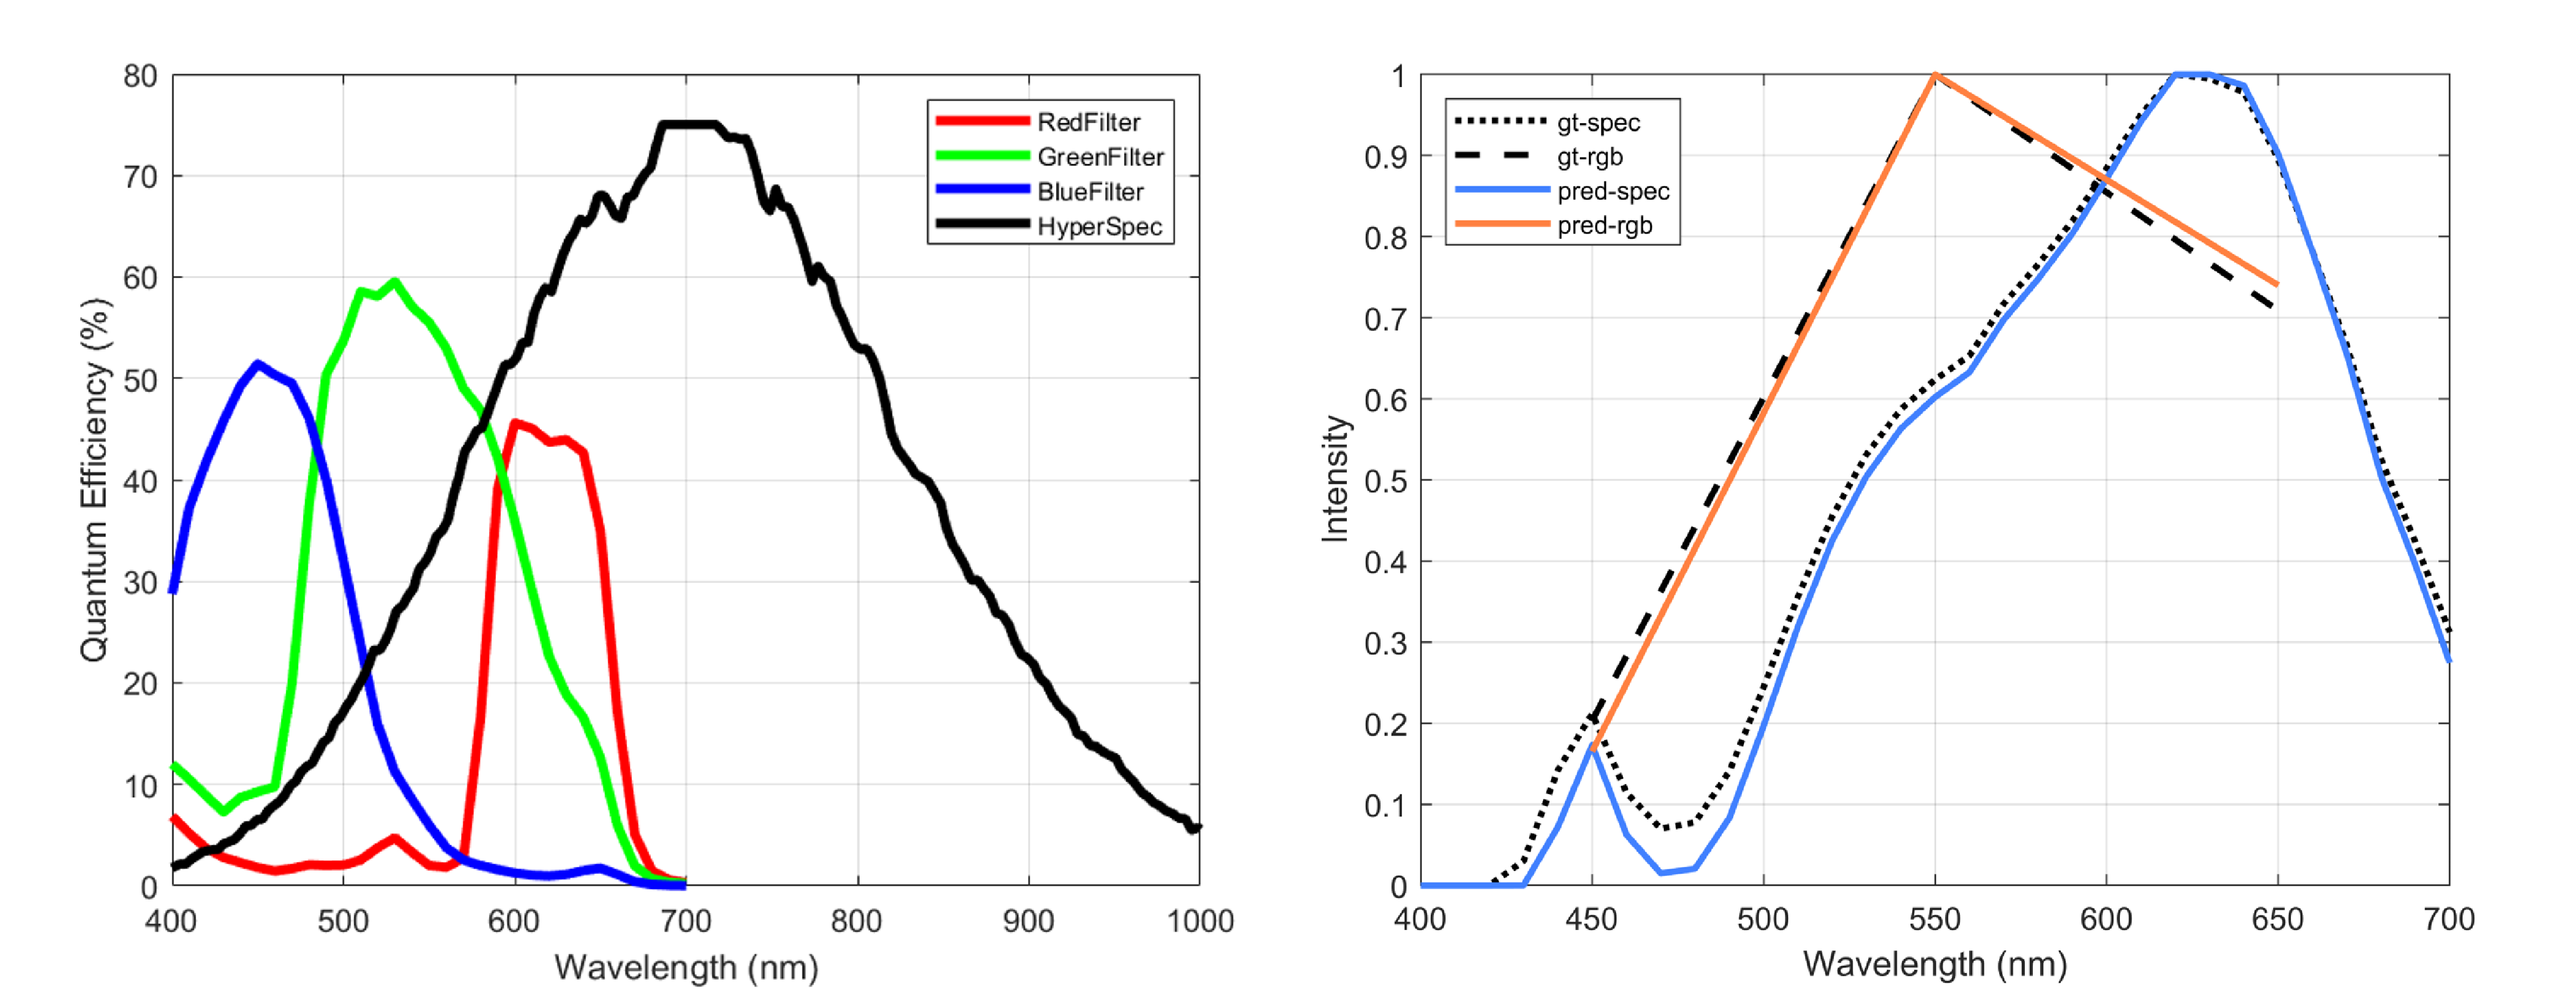
\includegraphics[width=1.0\linewidth]{docs/fig-chap2/fig-2-spec-rgb-compare.pdf}
	\end{center}
	\caption{左图:RGB 和高光谱相机的量子效率\quad 右图:RGB和高光谱域中光源估计的结果}
        \label{fig:spec-rgb}
\end{figure}

高光谱图像与RGB图像的差别不仅仅是通道数量的差别,高光谱相机的量子效率(Quantum Efficiency)曲线也与RGB相机的不同,如图\ref{fig:spec-rgb}左图所示。RGB 相机仅集成了三个宽谱波段,而高光谱相机则在更连续的光谱维度中采样信息,且高光谱相机的波段范围更大,涵盖700nm以上的近红外波段。

高光谱图像比RGB具有更丰富的光谱信息\cite{hardeberg2002multispectral},反映在单点的反射率或场景的光源光谱上时,RGB图像的光源光谱是一条只有三个采样点的折线,而光谱图像的光源光谱可以绘制为曲线。如图 \ref{fig:spec-rgb} 右图所示,黑色点线表示光源光谱真值曲线,黑色虚线表示光源RGB真值折线,蓝色曲线表示预测的光源光谱,橙色折线表示预测的光源光谱积分到RGB三通道后的颜色。这表明了,如果将预测的光源光谱积分到 RGB 的三个通道中,则预测的RGB光源更容易接近真实光源。此外,更多的光谱通道数会导致每个独立的光谱通道图像的信噪比降低,常见的做法是对多个高光谱通道的图像求平均,得到信噪比更高的多光谱图像。因此,高光谱光源估计问题比 RGB 域中的光源估计问题更加不确定和困难。

\subsection{真实数据集}

在现有的高光谱图像数据集中,为了凸显数据的多样性,光源的类型和强度对在同一场景获取的高光谱图像的影响尚未得到充分的研究。 因此,本文构建了一个在受控场景中切换光源类型和强度的数据集。 

\begin{figure*}[h]
	\centering
	%\fbox{\rule{0pt}{2in} \rule{0.9\linewidth}{0pt}}
	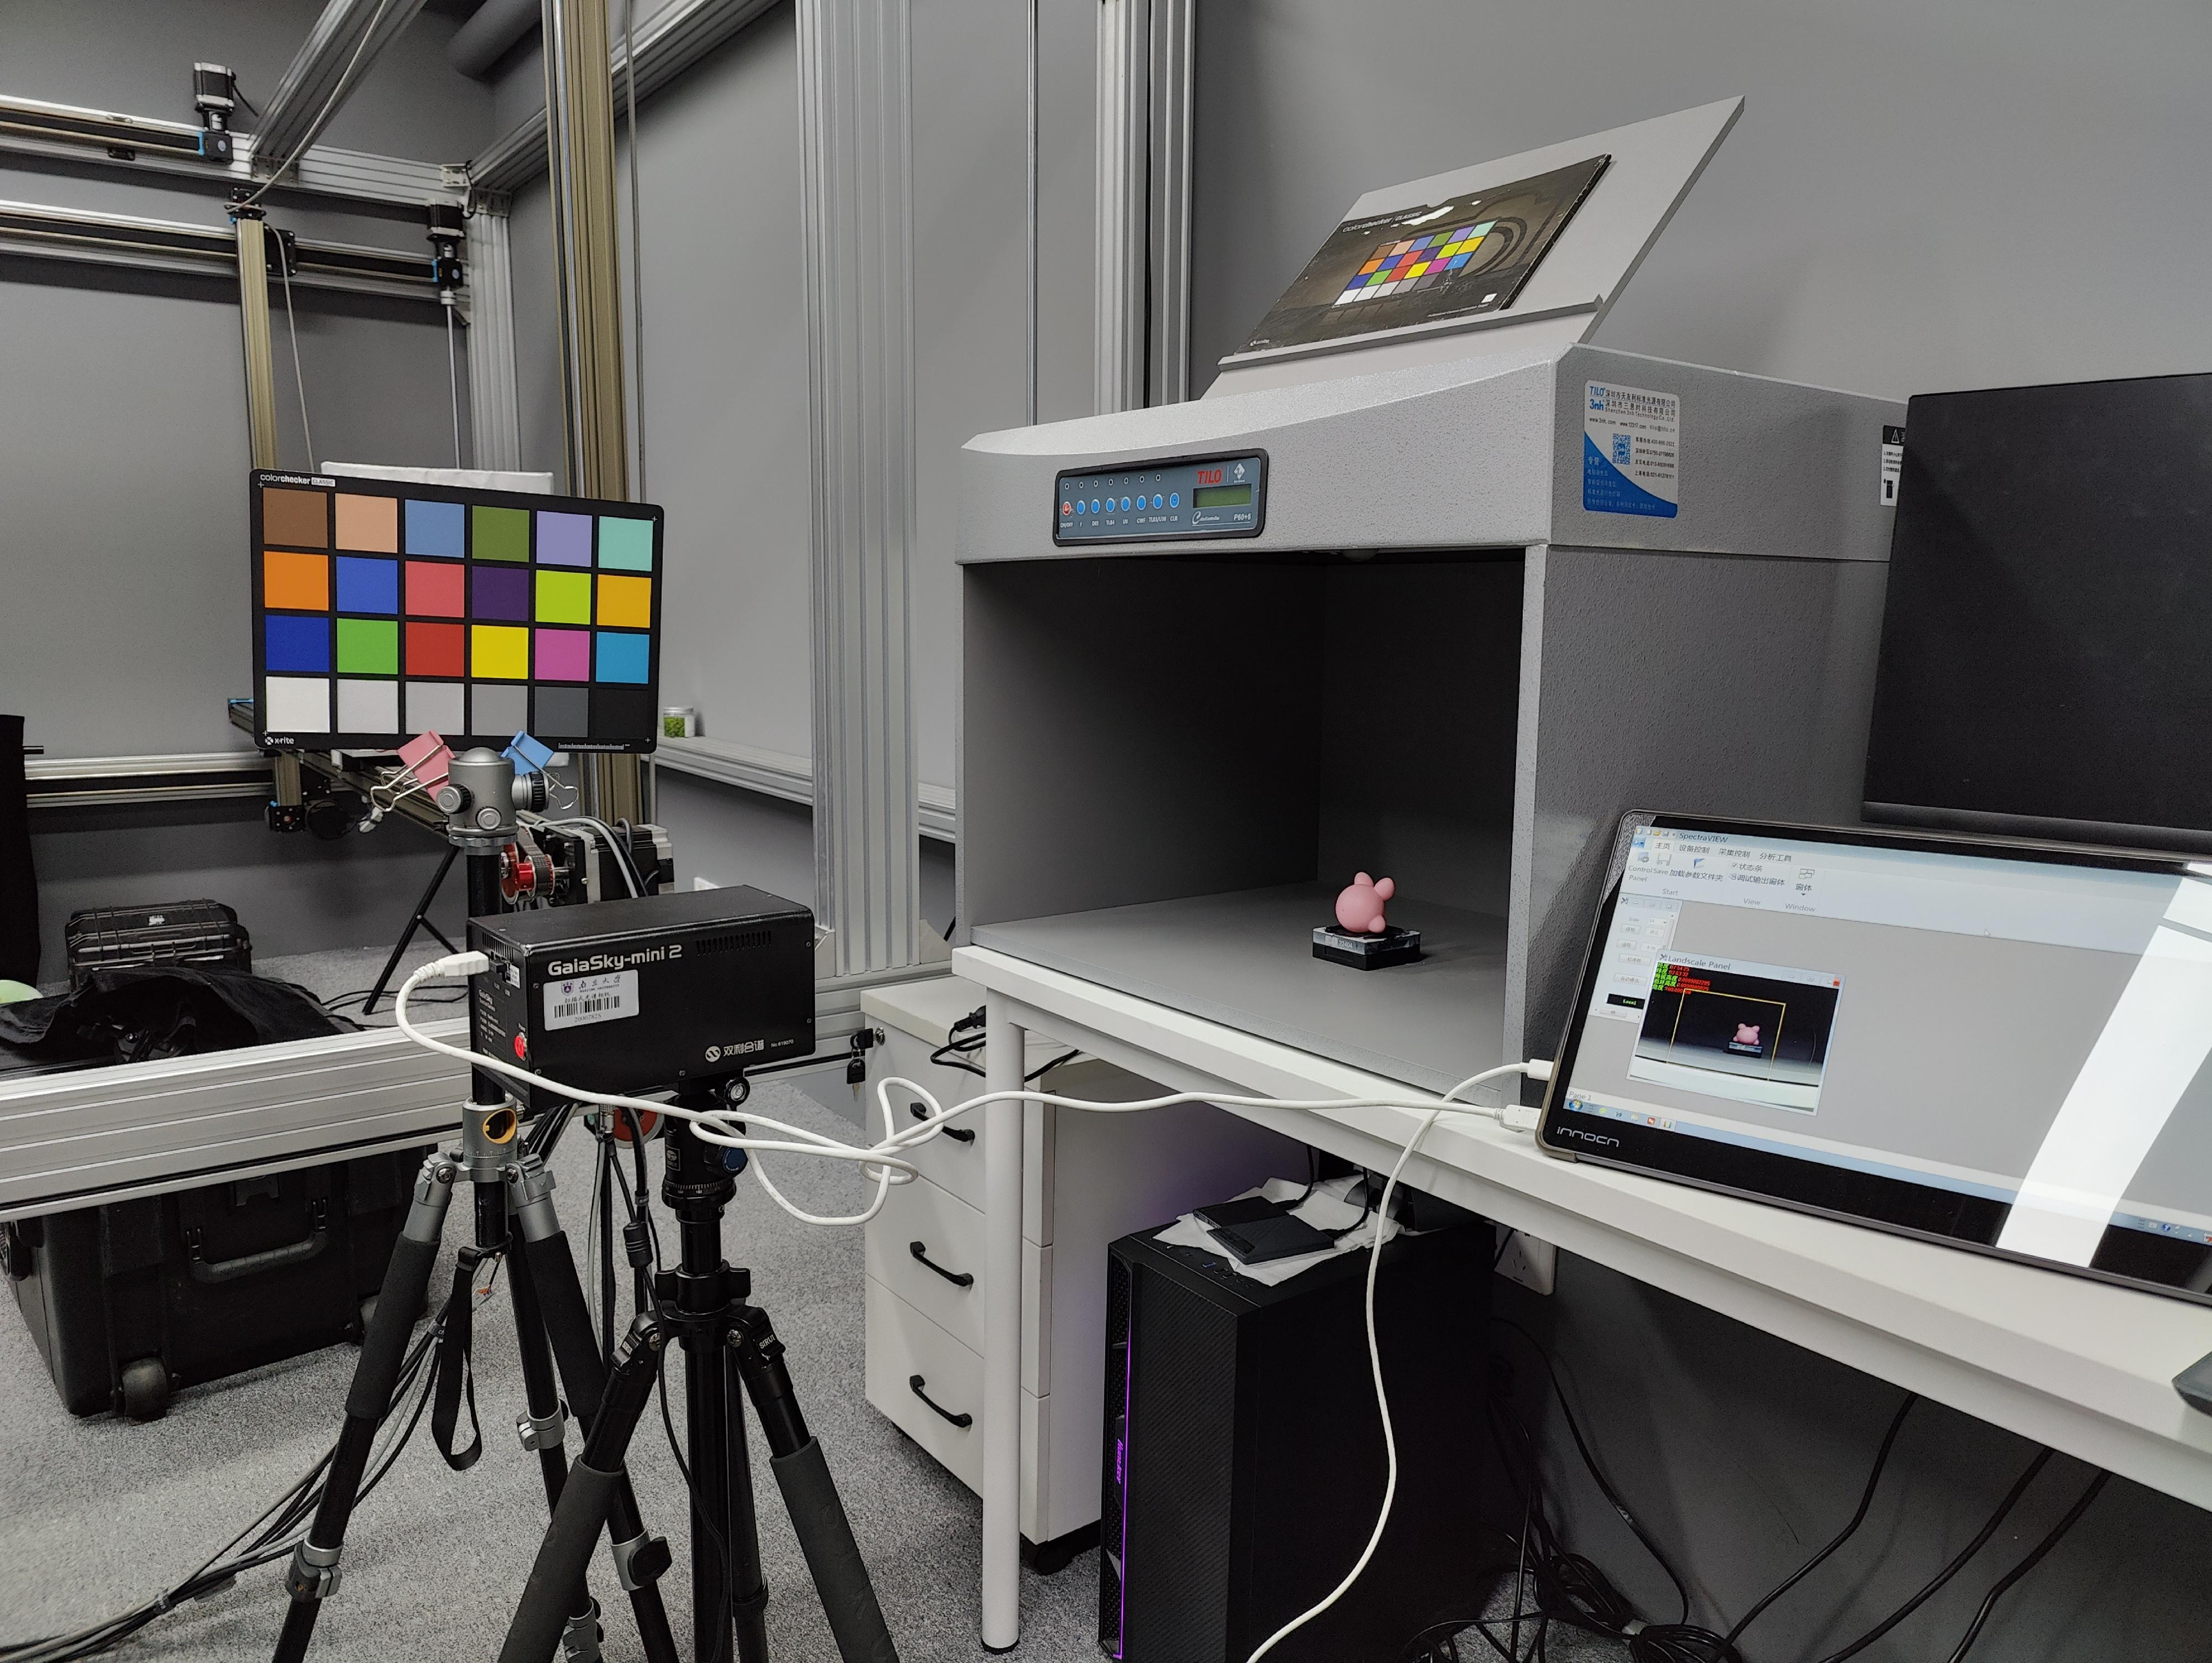
\includegraphics[width=0.8\linewidth]{docs/fig-chap2/fig-2-system.pdf}
	\caption{高光谱图像采集系统}
	\label{fig:system}
\end{figure*}

本文的数据集是使用推扫式高光谱相机 GaiaSky-Mini2 捕获的,拍摄时的设置及参数值如表\ref{tab:illum capture param}所示。高光谱图像原始尺寸宽$\times$高$\times$通道数为1057$\times$960$\times$176,光谱波段范围从390nm到1000nm。 由于本文使用的室内光源不包含近红外波段,将获取到的图像中大于770nm波段的通道图像舍弃,并对多个高光谱通道的图像求平均,减少波段数量,提高信噪比。处理后图像尺寸变为宽$\times$高$\times$通道数为1057$\times$960$\times$38,范围从400nm到770nm,间隔10nm。 

\begin{table}[h]
\caption{光源光谱估计数据集拍摄设置及参数值 }
\label{tab:illum capture param}
\begin{tabular}{ll}
\hline
拍摄设置   & 参数值     \\ \hline
高光谱相机镜头焦距 & 16mm \\
高光谱相机数值孔径    & F/2.8   \\
相机距拍摄画面中心距离 & 0.5m  \\
光源距拍摄画面中心距离  & 0.3m  \\
光源照射方向   & 单侧水平照射     \\
\hline
\end{tabular}
\end{table}

该数据集包含 18 个场景,全部在暗室环境中捕获,以确保光源条件可控。场景中的物体包括真假绿植、真假食物、玩偶、木质品、金属制品、石制品、皮肤、毛发等。 本文使用了 5 种不同的光源,挑选自常见的室内照明,色温范围为 2500K 至 6500K,如图\ref{fig:dataset}所示。 每个光源都以4个强度级别(从100lux到1000lux)捕获,总共生成 360 张高光谱图像。该数据集已经公布,可用于非商业目的的学术研究。

\begin{figure*}[h]

    \includegraphics[width=\linewidth]{docs/fig-chap2/fig-2-dataset.pdf} % 替换为
  \caption{本文构建的数据集\quad 左:光源色温为 6500K 的部分场景的RGB渲染图\quad 中:光源光谱\quad 右:同一场景在光源色温范围为 5500K 至 2500K 时的RGB渲染图}
  \label{fig:dataset}
\end{figure*}


如表\ref{tab: illumination datasets}所示,本文提出的真实数据集与常用的高光谱图像数据集相比,有更大光谱波段范围,校正方式包括标准24色卡和白板,仅在室内光源下拍摄。

\begin{table*}[h]
\centering
\caption{高光谱图像或光源数据集的比较}
\label{tab: illumination datasets}
\begin{tabular}{cccc cccc}
\hline
发布时间 & 名称 & 数量 & 分辨率 & 波段  & 校正方式 & 光源       \\
\hline
2002 &  SFU\cite{barnard2002data}%\textsuperscript{1} %\footnotemark
& \textbf{1995}     & \textbf{1$\times$1$\times$101}      & 380-780nm              &  \textbf{直接测量}    & 室内 \& 室外 \\
2008 & CAVE\cite{yasuma2010generalized}%\textsuperscript{2} %\footnotemark
& 32       & 512$\times$512$\times$31            & 400-700nm              &  色卡    & 室内             \\
2011 & Harvard\cite{chakrabarti2011statistics}%\textsuperscript{3} %\footnotemark
& 75       & 1040$\times$1392$\times$31          & 420-720nm             &  无      & 室内 \& 室外 \\
2014 & NUS\cite{nguyen2014training}
&64 & 984$\times$1312$\times$31 & \textbf{400-1000nm}    &  色卡    & 室内 \& 室外     \\    
2015 & Foster\cite{nascimento2016spatial}%\textsuperscript{4} %\footnotemark
& 30       & 1018$\times$1339$\times$33          & 400-720nm              & \textbf{漫反射球}     & 室外           \\
2017 & KAIST\cite{choi2017high}%\textsuperscript{4} %\footnotemark
& 30       & \textbf{3376$\times$2704$\times$31}          & 420-720nm              & 色卡     & 室内           \\
2021 & KAUST\cite{li2021multispectral}%\textsuperscript{5} %\footnotemark
&  \textbf{409}      & 512$\times$512$\times$31            & 400-730nm              &  白板    & 室内 \& 室外 \\
2022 & NTIRE\cite{arad2022ntire}%\textsuperscript{6} %\footnotemark
& \textbf{1000}     & 482$\times$512$\times$31            & 400-700nm               &  无    & 室内 \& 室外 \\
2024 &  本数据集 & \textbf{360}      & 960$\times$1057$\times$38 & 400-770nm    &  色卡+白板    & 室内     \\       
\hline
\end{tabular}
\end{table*}


\subsection{仿真数据集}
% \begin{figure*}[h]
%     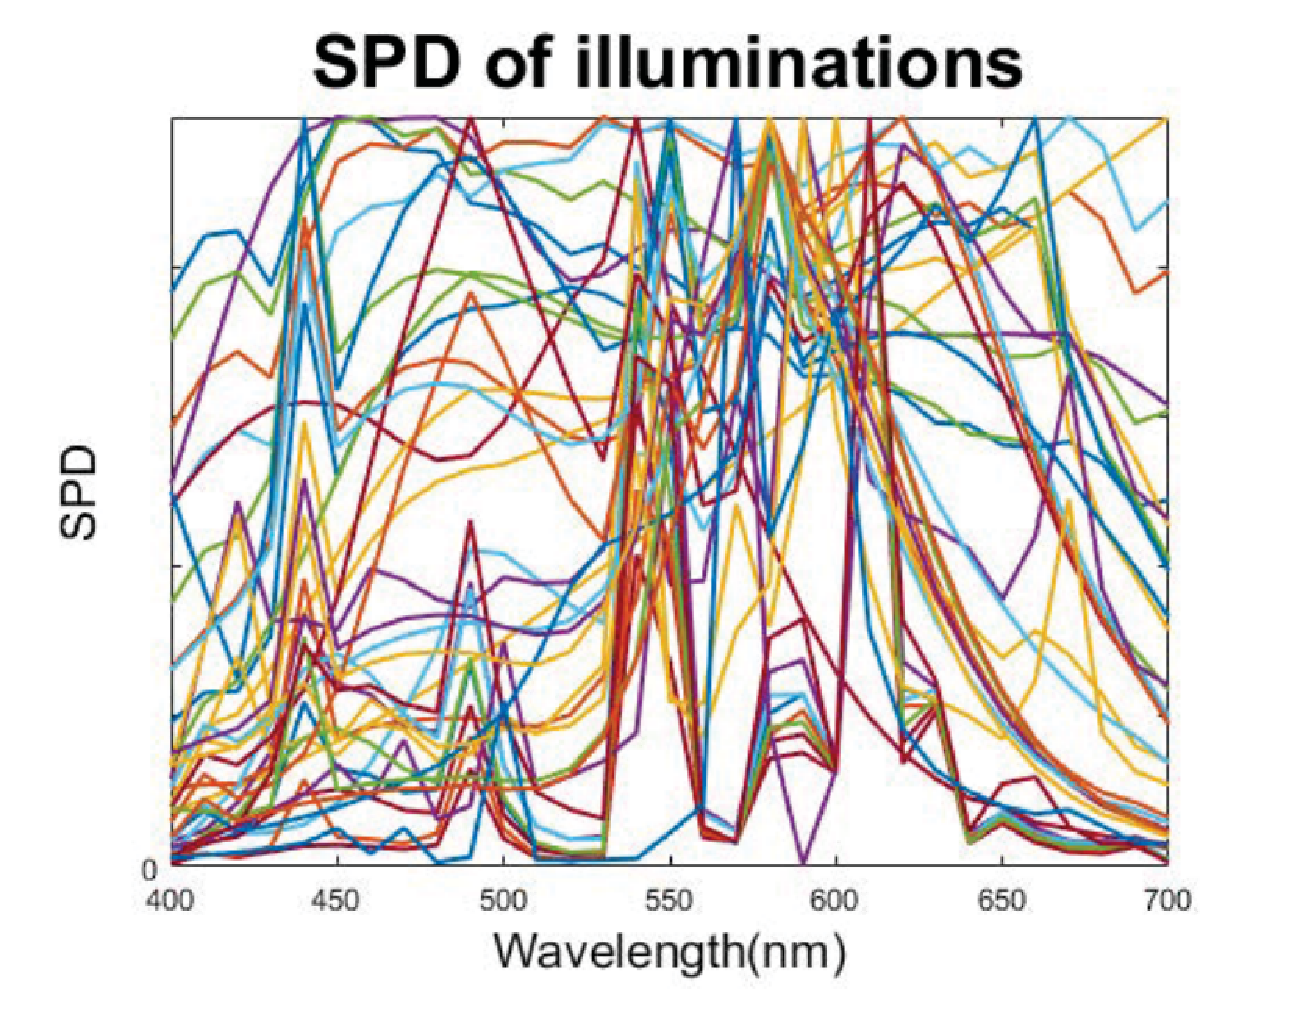
\includegraphics[width=\linewidth]{docs/fig-chap2/fig-2-dataset-spd.pdf} % 替换为
%   \caption{仿真数据集使用的光源能量分布曲线。}
%   \label{fig:dataset spd}
% \end{figure*}
为了进一步增强训练场景的多样性,特别是对室外场景的补充,本文使用 KAUST\cite{li2021multispectral} 提出的高光谱反射率数据集和 SFU\cite{barnard2002data} 提出的光源光谱数据集合成仿真数据集。 KAUST 的数据集由 400 张高光谱图像组成,包括室内场景和室外场景,尺寸为 512 $\times$ 512 $\times$ 31,光谱波段范围从 400nm 到 700nm,光谱分辨率为10nm。 SFU 的数据集包含 102 条光源光谱曲线,包括室内光源和太阳光,每条曲线有 101 个波段,光谱波段范围从 380nm 到 780nm,光谱分辨率为4nm。 本数据集截取其中的 400nm 至 700nm 范围,以 10nm 间隔对其进行下采样,以获得 31 个波段的光源曲线。按照$\mathbf{I} = \mathbf{R}\cdot L$,其中$\cdot$表示点积,将处理后的SFU数据集中的光源光谱$L$与 KAUST数据集提供的反射率$\mathbf{R}$相乘,以合成仿真的高光谱图像$\mathbf{I}$,构成仿真数据集。仿真的高光谱图像$\mathbf{I} \in \mathbb{R}^{H \times W \times C}$,其反射率图像为 $\mathbf{R} \in \mathbb{R}^{H \times W \times C}$,其中$H$是高度,$W$是宽度,$C$是通道数,光源光谱为$L \in \mathbb{R}^{C}$,意味着这是一个全局一致的光源光谱估计数据集。筛选掉一些重复场景后,总共使用了384张高光谱图像进行训练和验证。


\section{本文提出的方法}
\begin{figure*}[h]
	\centering
	%\fbox{\rule{0pt}{2in} \rule{0.9\linewidth}{0pt}}
	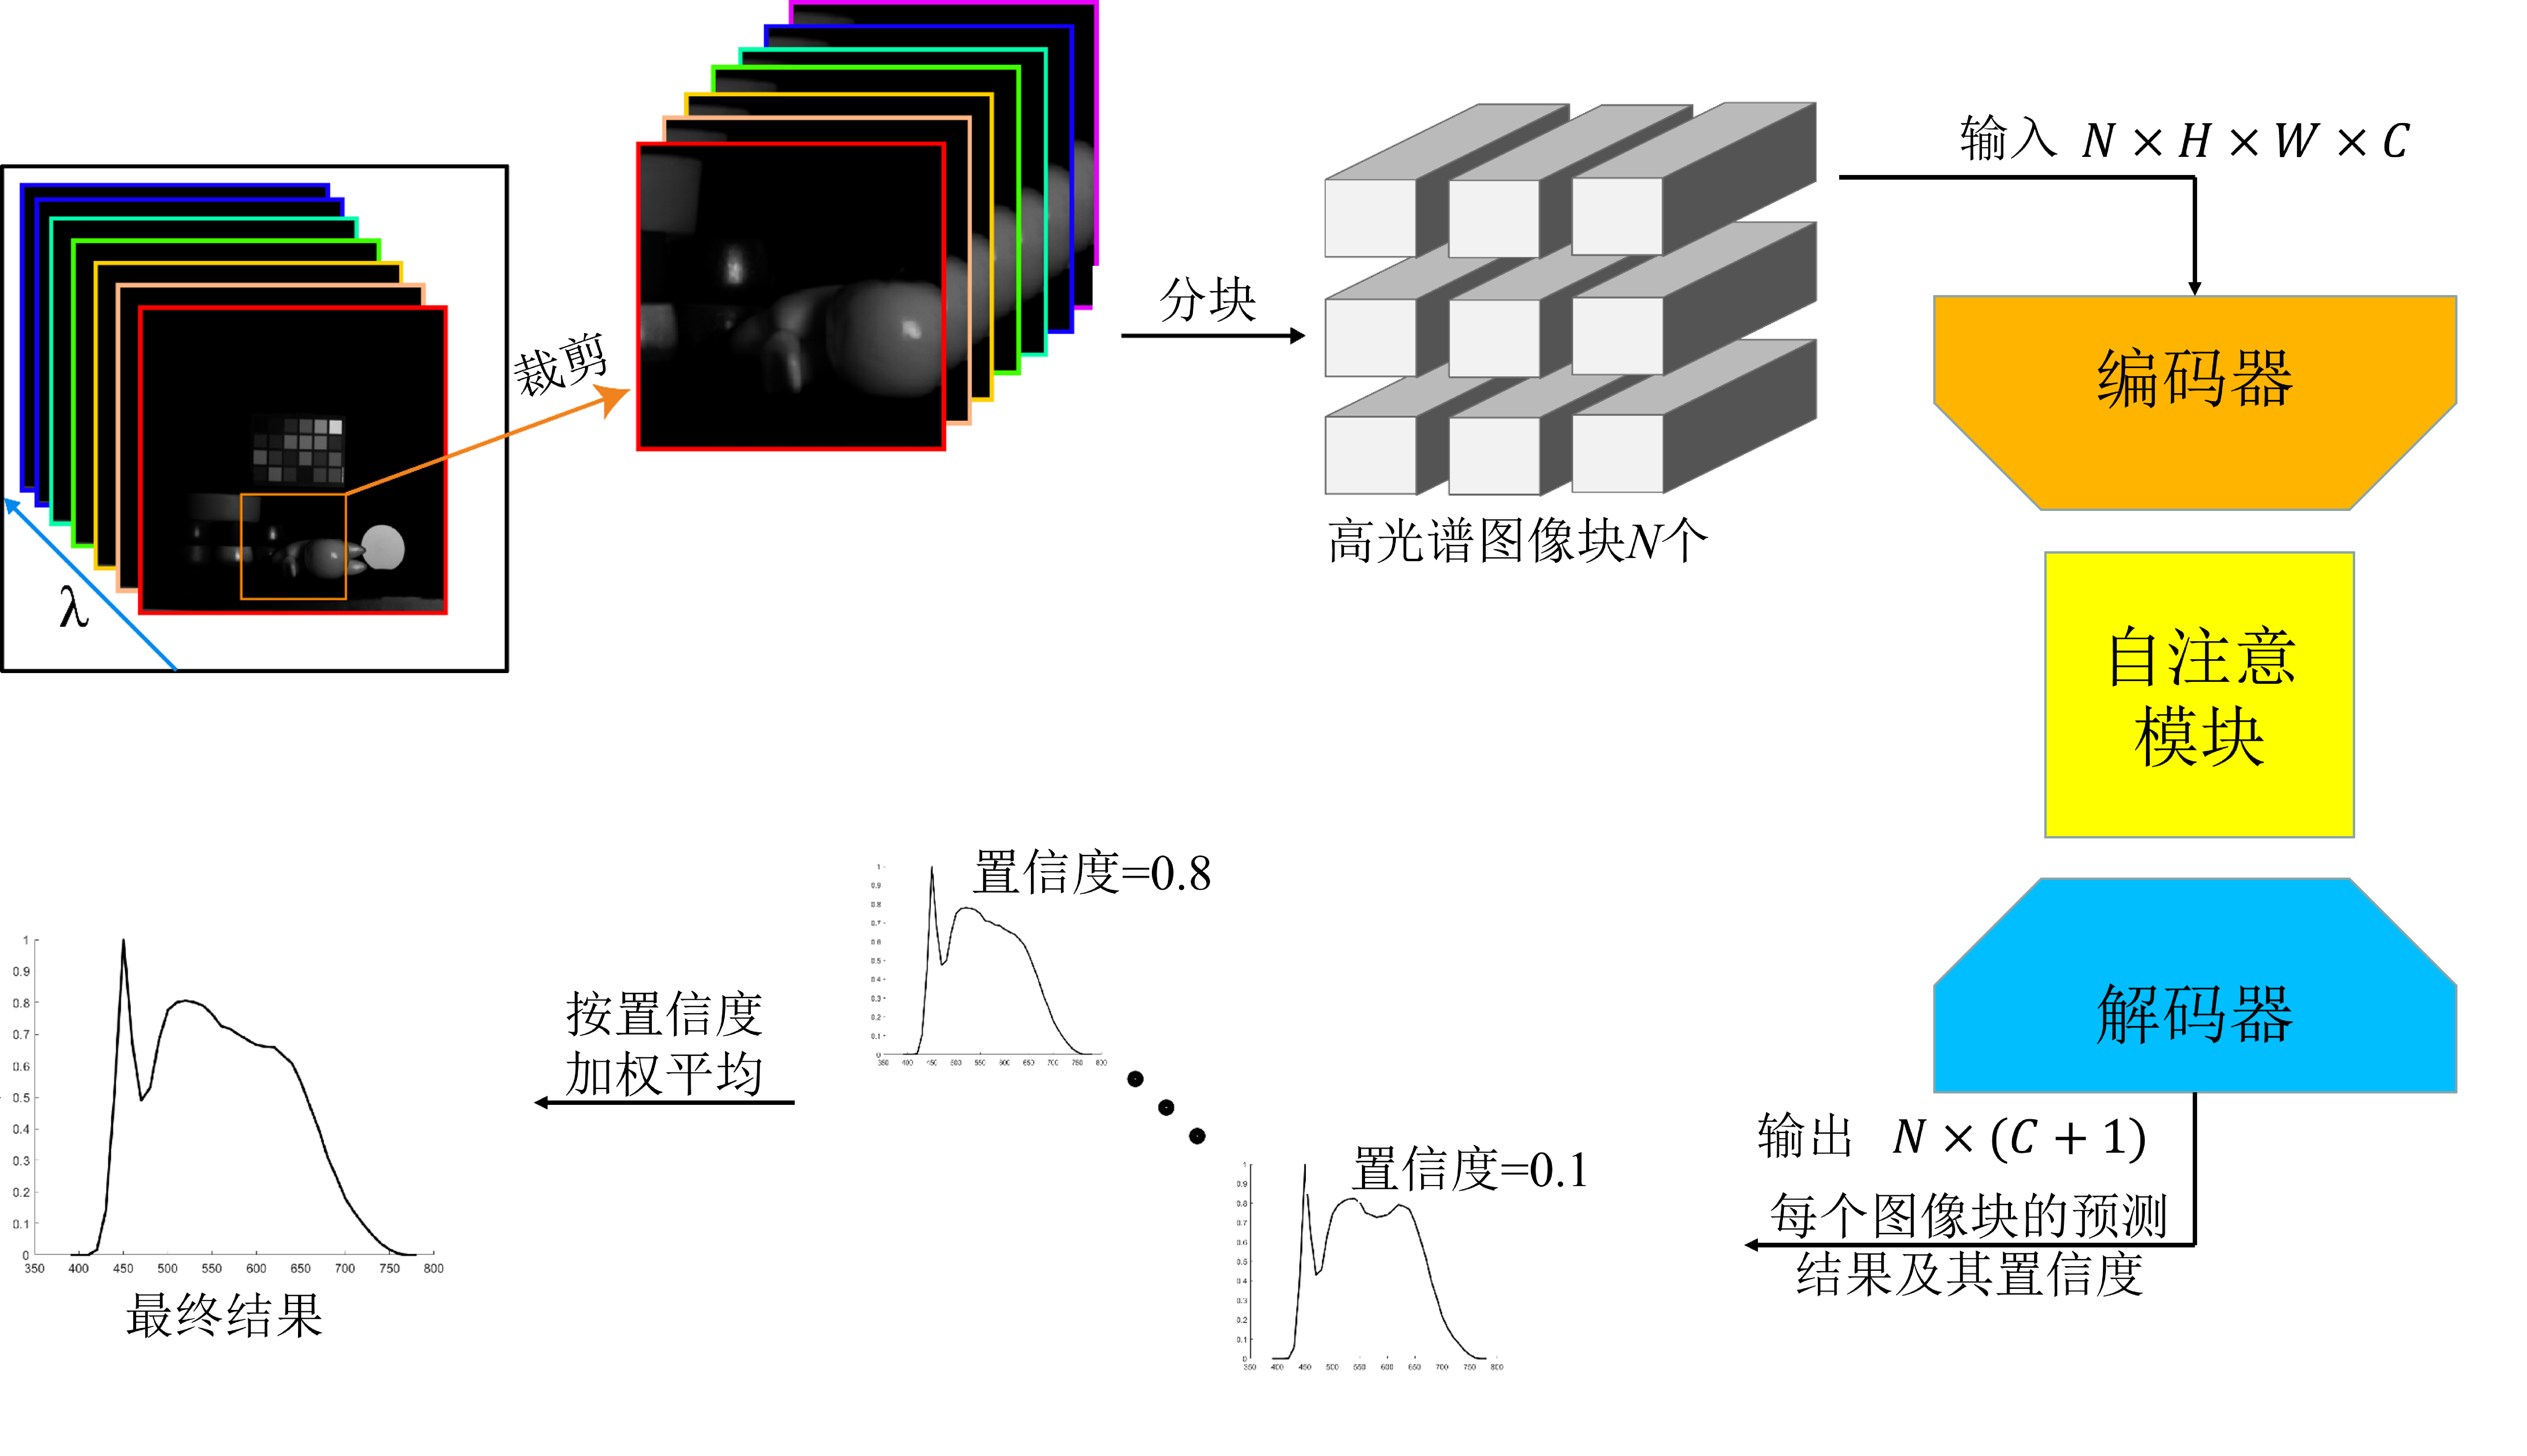
\includegraphics[width=1.0\linewidth]{docs/fig-chap2/fig-2-pipeline-u.pdf}
	\caption{算法处理流程\quad }
	\label{fig:pipeline}
\end{figure*}
对于全局光源估计的任务,本文设计了一个算法处理流程,如图\ref{fig:pipeline}所示。采用Transformer的编码器和解码器,网络参数设置如表\ref{tab:illum net param}所示,并在其中加入光谱联合空间自注意模块,在损失函数中添加平滑约束。

考虑到高分辨率的高光谱图像在模型训练时会占用大量显存空间,本文将输入的高光谱图像首先沿空间维度分割成大小相等的高光谱图像块,并且假设每个高光谱图像块包含完整的光源光谱。 这些高光谱图像块将被输入到模型中,模型分别输出相应的预测光源光谱和置信权重。 最后根据置信度权重进行加权平均,得到预测的全局光源光谱。 

\begin{table}[h]
\caption{光源光谱估计网络参数设置 }
\label{tab:illum net param}
\begin{tabular}{ll}
\hline
网络参数   & 参数值     \\ \hline
等边图像尺寸 & 512\times 512 \\
等边图像块尺寸   & 8\times 8   \\
为每一个图像块编码的长度  & 31  \\
编码器深度   & 6  \\
多头注意力中头的数目  & 2     \\
多层感知器中隐含层的维度  &  512 \\
随机数种子编号  &  42 \\
\hline
\end{tabular}
\end{table}

% 对于$\left\{\mathbf{P}_{(i)}\right\}_{i=0, \ldots, K^-1}$

在训练期间,将每个图像块与真实测量值进行比较以计算损失。 在测试过程中,将预测的全局光源光谱与真实测量值进行比较,进而获得角误差和均方差。在训练和测试时,使用0-1掩膜将图像中的色卡和白板遮盖,避免模型直接从色卡或白板中学习光源光谱。

\subsection{光谱联合空间自注意}

考虑到Transformer 在捕获非局部远程依赖性方面的有效性及其在其他视觉任务中优越的性能,本文的目标是探索 Transformer 在高光谱光源估计中的潜力。 然而,直接将 Transformer 应用到高光谱光源估计时存在两个主要问题。 

第一个问题是原始的Transformer 在空间维度上的建模依赖于远程关系\cite{cai2022mask}。 另一个问题是高维数据的参数量太大,无法直接输入到自注意模块中。 

\begin{figure}[h]
	\begin{center}
		%\fbox{\rule{0pt}{2in} \rule{0.9\linewidth}{0pt}}
		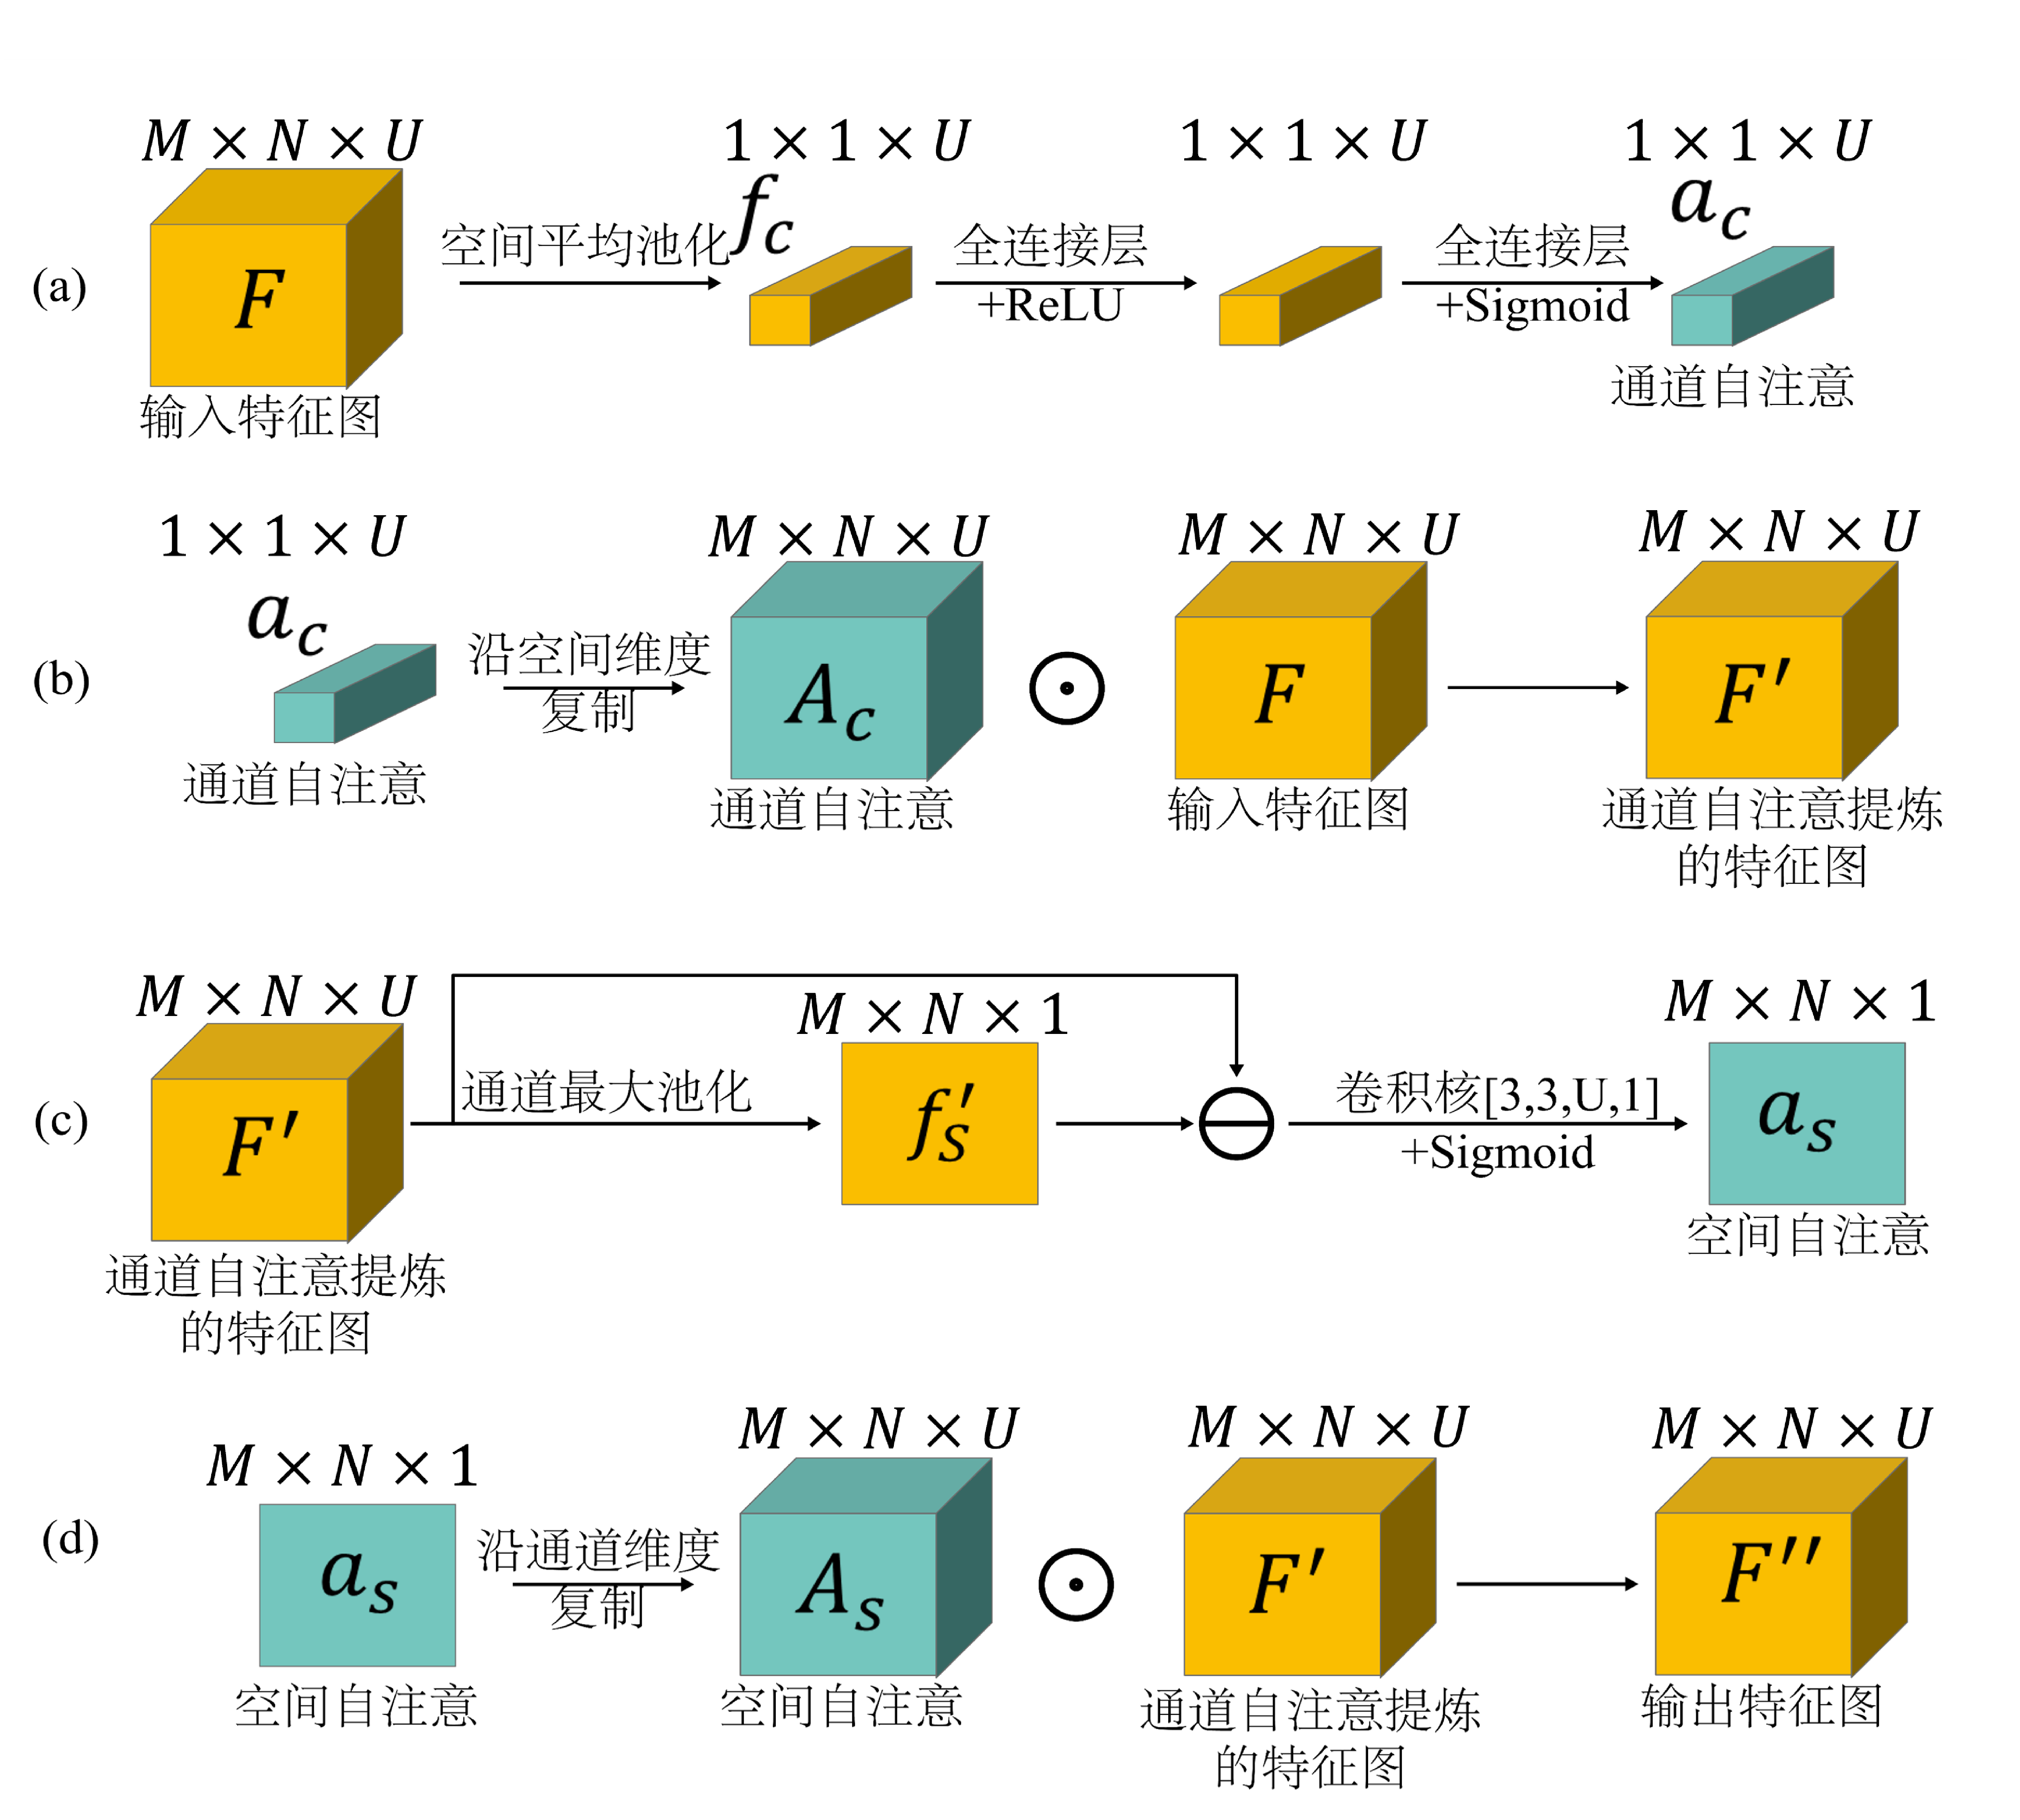
\includegraphics[width=1.0\linewidth]{docs/fig-chap2/fig-2-attention.pdf}
	\end{center}
	\caption{光谱联合空间自注意模块\quad (a)提取通道自注意\quad (b)将通道自注意作用于特征图 \quad (c)提取空间自注意\quad (d)将空间自注意作用于特征图}
	\label{fig:attentionn}
\end{figure}

本文设计了包含四个步骤的自注意模块,如图\ref{fig:attentionn}所示,特征图和自注意使用不同的颜色加以区分。该模块包含两方面的自注意操作:通道自注意和空间自注意。通道自注意用于增强或抑制不同通道的信息,而空间自注意用于强调或削弱特定位置的信息。

对于通道自注意,首先通过全局平均池化,计算输入特征的全局平均值,然后使用两个全连接层计算通道权重。 第一个全连接层使用ReLU激活函数,第二个全连接层使用Sigmoid激活函数,输出通道自注意。 这种方法允许网络专注于特定的通道。
% 通道自注意允许网络沿着通道维度了解特定通道的重要性。

如图\ref{fig:attentionn}(a)所示,将从特征图中提取通道自注意的过程可以表示为:
\begin{equation}
    \begin{align}
        f_c[u] &= \frac{1}{M \times N} \sum_{m=0}^{M-1} \sum_{n=0}^{N-1} F[m,n,u],\\
        a_c[u] &= \text{Sigmoid}(w_2[u]\text{ReLU}(w_1[u]f_c[u] + b_1[u])+b_2[u]).
    \end{align}
\end{equation}

其中$F$为特征图,它的维度为 $M \times N \times U$,$M$ 是高度,$N$ 是宽度,$U$ 是通道数,$F[m,n,u]$表示矩阵$F$中$[m,n,u]$位置的元素,$f_c$为在沿空间维度平均池化后的特征,它的维度等于通道数$U$。$w_1$,$b_1$,$w_2$,$b_2$分别为第一个和第二个全连接层的权重和偏置,$a_c$表示维度为通道数$U$的通道自注意。

如图\ref{fig:attentionn}(b)所示,将通道自注意作用于特征图的过程可以表示为:
\begin{equation}
    \begin{align}
        A_c &= a_c\otimes M \otimes N,\\
        F^{\prime} &= A_C \odot F.
    \end{align}
\end{equation}

其中$\otimes$为Kronecker积,$A_c$为$a_c$沿着空间维度复制得到的维度为$M \times N \times U$的通道自注意。$\odot$表示矩阵的像素乘积,$F^{\prime}$为经过通道自注意提炼后的特征图。

对于空间自注意,首先计算通道自注意的最大值,然后使用3x3的卷积核进行卷积操作。 输入特征减去通道最大值得到的差值被输入到卷积运算中,然后通过Sigmoid函数进行缩放,从而产生空间自注意。 这种方法允许网络专注于图像中的特定区域。
% 空间自注意允许网络专注于图像中的特定区域。

如图\ref{fig:attentionn}(c)所示,从特征图中提取空间自注意的过程可以表示为:
\begin{equation}
    \begin{align*}
    &f^{\prime}_s[m,n] = \underset{u}{\operatorname{max}}(F^{\prime}[m,n,u]),\\
    &\Delta F^{\prime} = f_s \otimes U -F^{\prime},\\
    a_s[m,n] = \text{Sigmoid}&\left(\sum_{i=0}^{2} \sum_{j=0}^{2} \sum_{u=0}^{U-1}  w_3[i,j,u]\Delta F^{\prime}[m+i,n+j,u]+b_3[i,j,u]\right).
    \end{align*}
\end{equation}

其中$f^{\prime}_s$为$F^{\prime}$沿着通道维度最大值池化的结果,将$f^{\prime}_s$沿着通道维度复制,维度对齐于$F^{\prime}$后与之作差的结果为$\Delta F^{\prime}$。维度为$M\times N$的空间自注意$a_s$为$\Delta F^{\prime}$经过$3 \times 3 \times U \times 1$ 的卷积核以步长为1卷积并使用Sigmoid函数激活后得到,该卷积核在通道维度输入为$U$,输出为1,其权重为$w_3$,偏置为$b_3$。

如图\ref{fig:attentionn}(d)所示,将空间自注意作用于特征图的过程可以表示为:
\begin{equation}
    \begin{align}
        A_s &= a_s \otimes U, \\
        F^{\prime\prime} &= A_s \odot F^{\prime}.
    \end{align}
\end{equation}

其中$A_s$为为$a_s$沿着通道维度复制得到的维度为$M \times N \times U$的空间自注意。$F^{\prime\prime}$为光谱联合空间自注意模块最终输出的特征图。

% 最后,光谱联合空间自注意模块,输出与通道和空间自注意融合的特征$F^{\prime\prime}$。
该自注意模块可以嵌入深度学习网络中,以增强网络对特定通道和位置信息的感知。
\subsection{平滑约束的损失函数}
在之前的研究中,基于角误差的损失函数通常优于基于均方差的损失函数。此外,本文引入了平滑损失以适应自然光和白色节能灯的光谱特征。 平滑损失通过计算光源光谱的二阶导数来衡量,总体损失函数可以表示为:
\begin{equation}\label{loss}
\ell  = {e_{angular}} + \eta {\ell
_{smooth}}.
\end{equation}

其中${e_{angular}}$为预测的光源光谱与光源光谱真实值的角误差,$\ell_{smooth}$为平滑损失项,$\eta$为平滑系数。

平滑损失项通过以下方式计算:
\begin{equation}\label{smooth loss}
\begin{align}
{\Delta ^2}[L](\lambda) &= L(\lambda  + 2)-2L(\lambda  + 1) + L(\lambda),\\
% \end{equation}
% \begin{equation}\label{second diff}
    \ell_{smooth} &=
\frac{1}{C}\|{{\Delta ^2}[L](\lambda)}\|^2.
\end{align}
\end{equation}

其中$C$表示光谱通道数,$\lambda$是离散的光谱通道。 $\|\cdot\|$表示L-2范数,${\Delta ^2}$表示光源$L$的二阶导数。

\section{实验过程与结果分析}
\subsection{实验设置 }
% 本文光源光谱估计模型由PyTorch框架实现,
本文的深度学习算法训练和测试,均在一台搭载了Intel Xeon Gold 6510处理器(2.70 GHz)、125GB内存、2块NVDIA RTX3090显卡(每块显卡显存24GB)的远程服务器中完成。对于软件系统,在AMD64架构的Linux系统Ubuntu 20.04.6 LTS平台下运行Docker 25.0.0完成容器搭建。在容器中,在Ubuntu 18.04.5 LTS平台下使用conda 4.10.1管理深度学习环境,主要包括python 3.9.6和pytorch 1.8.1,使用cuda 11.1将模型部署于显卡。

实验结果的数据分析在一台搭载了12代Intel Core i7-12800HX处理器(2.00 GHz)、64GB内存、NVIDIA RTX A1000显卡(显存4GB)的笔记本电脑中完成。对于软件系统,在64位Windows 11 Pro 23H2系统下运行MATLAB R2022a。

训练和测试阶段的参数设置如表\ref{tab:illum param}所示。由于本文构建的真实数据集的每个场景包括20张在不同光源种类及强度的光源下拍摄,数据间的相似度较高,在此数据集内训练并测试不足以说明模型的泛化性。因此,本文在仿真场景实验与真实场景实验中同样使用仿真数据集中的288张高光谱图像训练,在测试时分别在各自的数据集中测试。

\begin{table}[h]
\caption{光源光谱估计实验设置及参数值 }
\label{tab:illum param}
\begin{tabular}{ll}
\hline
实验参数   & 参数值     \\ \hline
深度学习框架 & PyTorch \\
优化器    & Adam   \\
初始学习率  & 0.001  \\
权重衰减   & 0.0005  \\
训练轮数   & 3000     \\
批大小    & 16       \\ 
用于训练的样本数量  &  288 \\
用于测试的样本数量  &  仿真场景96,真实场景360 \\
\hline
\end{tabular}
\end{table}

\subsection{评价指标}
光源估计通常分为两种类型:全局光源估计和像素级光源估计。 

本文在设计实验时,专注于讨论全局光源估计,这种方法可用作白板等光源参考的有效替代。

本文使用角误差$e_{angular}$和均方差$e_{msquare}$两种评价指标对光源光谱估计的结果进行评价,角误差的计算方式为:
\begin{equation}\label{angular error}
{e_{angular}}(L, \hat{L}) = \arccos\left(\frac{\langle{L}, \hat{L}\rangle}{\|{L}\|\|\hat{L}\|}\right).
\end{equation}

均方差的计算方式为:

\begin{equation}\label{$e_{msquare}$}
{e_{msquare}}(L, \hat{L}) = \frac{1}{C}\sum\limits_{\lambda  = 1}^C {{{\left({L(\lambda)-\hat L(\lambda)} \right)}^2}}.
\end{equation}

其中$L$是预测的光源光谱,$\hat{L}$是光源光谱真实值,本文中角误差统一用角度制表示。

光源光谱估计旨在最小化预测光源矢量与真实光源矢量之间的误差。 需要注意的是,在高光谱图像处理中,图像通常被全局归一化,从而获得无单位的反射率图,仅保留像素之间的相对强度而非绝对强度,因此,不受光源绝对强度影响的角误差更适用于高光谱图像光源估计结果的评估。


\begin{figure*}
	\centering
	%\fbox{\rule{0pt}{2in} \rule{0.9\linewidth}{0pt}}
	\includegraphics[width=0.8\linewidth]{docs/fig-chap2/fig-2-result.pdf}
	\caption{仿真场景实验结果可视化}
	\label{fig:simulated result}
\end{figure*}

\subsection{仿真场景实验 }

在仿真场景实验中,本文使用仿真数据集共384张高光谱图像中的75\%用于训练,剩余的25\%用于测试。将本文提出的方法与其他方法进行对比,包括基于统计的方法(Spectral Gray World、Max Spectral、Spectral Gray Edge\cite{RN17} 和 镜面反射分解\cite{RN35})以及基于学习的方法(PixelWise Illuminant Recovery (PWIR)\cite {RN24}和深度展开网络\cite{li2021multispectral})。PWIR中使用了浅层的AlexNet,为了更公平地对比,额外测试了用resnet50取代AlexNet的效果。其余对比算法的参数设置均固定采用相应论文中的默认设置。

\begin{table}[h]
\centering                % 表格居中
\caption{不同算法在仿真数据集上的比较} 
\label{tab:illu syn}
\begin{tabular}{l|llll llll}
\hline
\multirow{2}{*}{方法} & \multicolumn{4}{c}{角误差/度}                                           & \multicolumn{4}{c}{均方差}                                           \\
                    & 平均值            & 中位值            & 最小值            & 最大值            & 平均值            & 中位值            & 最小值            & 最大值            \\ \hline
Gray World          & 25.19          & 23.45          & 0.845          & 73.59          & 0.154          & 0.142          & 0.015          & 0.312          \\
Max Spectral            & 22.95          & 21.17          & 0.662          & 65.71          & 0.141          & 0.121          & 0.011          & 0.300          \\
Gray Edge           & 22.94          & 21.08          & 0.716          & 65.75          & 0.142          & 0.125          & 0.012          & 0.298          \\
镜面反射分解                & 25.16          & 23.57          & 0.805          & 69.01          & 0.148          & 0.129          & 0.015          & 0.308          \\
深度展开网络               & 19.14          & 16.53          & 3.952          & 56.51          & 4.318          & 3.871          & 2.305          & 6.832          \\
PWIR-alexnet      & 8.649          & 6.976          & 0.607          & 49.48          & 2.362          & 1.824          & 0.493 & 5.209          \\   
PWIR-resnet50      & 5.415          & 4.440          & 0.608          & 22.68          & 0.018          & 0.005          & \textbf{0.000}          & 0.060          \\
本文提出的方法                 & \textbf{3.841} & \textbf{2.709} & \textbf{0.088} & \textbf{24.05} & \textbf{0.014} & \textbf{0.001} & \textbf{0.000} & \textbf{0.050} \\ \hline
\end{tabular}
\end{table}



如表\ref{tab:illu syn}所示,在合成数据集上,本文提出的方法得到的光源光谱估计的准确性在角误差$e_{angular}$ 和均方差$e_{msquare}$ 指标上都显着优于以前的方法。对于仿真场景实验,在本文提出的方法得到的结果中,平均角误差约为3.8度,相比平均角误差约为5.4度的PWIR-resnet50方法降低了约29\%;而基于统计的方法得到的平均角误差约为25度左右。


如图\ref{fig:simulated result}所示,基于统计的方法估计出的光源光谱曲线更容易偏离真实的光源光谱且具有类似的趋势,而基于学习的方法的估计具有另一种类似的趋势,并且基于学习的方法普遍优于基于统计的方法。 值得注意的是,由于引入了平滑损失,本文提出的方法在光源曲线中具有峰值的光源(例如 LED)和具有平滑光谱曲线的光源(例如自然光、白炽灯)的两种情况下的光源光谱估计都表现良好。从如图\ref{fig:simulated result}的第2、3行可以看到,本文提出的方法对光谱曲线中带有尖峰的光源估计得更准,而对第1、4行中不带有尖峰的光源的估计有明显的偏差,可能的原因是带有尖峰的曲线的特征更易于表示。

\subsection{真实场景实验 }

以往的研究普遍缺少真实场景的实验,原因在于:一、室外场景很难在改变光源条件的同时保证场景中物体位置不变化;二、购买多种光源的成本较高且拍摄更复杂。

为了更有效的评估各种光源估计方法,本实验在室内用5种不同的光源进行拍摄,虽然光源种类不如仿真实验的101种光源多,但都是实际室内光源中经常使用的,有一定的代表性。

\begin{table}[h]
\centering                % 表格居中
\caption{不同算法在真实数据集上的比较} 
\label{tab:illu real}
\begin{tabular}{l|llll llll}
\hline
\multirow{2}{*}{方法} & \multicolumn{4}{c}{角误差/度}                                           & \multicolumn{4}{c}{均方差}                                           \\
                    & 平均值            & 中位值            & 最小值            & 最大值            & 平均值            & 中位值            & 最小值            & 最大值            \\ \hline
Gray World          & 29.32          & 27.29          & 0.983          & 85.65          & 0.177          & 0.163          & 0.017          & 0.358          \\
Max Spectral            & 23.9           & 22.04          & 0.689          & 68.43          & 0.143          & 0.122          & 0.011          & 0.304          \\
Gray Edge           & 36.82          & 33.83          & 1.149          & 105.5          & 0.195          & 0.171          & 0.016          & 0.409          \\
镜面反射分解                & 33.49          & 31.37          & 1.071          & 91.85          & 0.18           & 0.156          & 0.018          & 0.374          \\
深度展开网络               & 25.14          & 21.71          & 5.190          & 74.22          & 0.159          & 0.142          & 0.084          & 0.251          \\
PWIR-alexnet        & 14.18          & 11.43          & 0.995          & 81.12          & 0.092          & 0.071          & 0.004          & 0.202          \\    
PWIR-resnet50   & 6.693          & 5.487          & 0.751          & 28.03          & 0.039          & 0.030          & 0.019          & 0.13           \\
本文提出的方法                 & \textbf{4.485} & \textbf{3.163} & \textbf{0.102} & \textbf{28.08} & \textbf{0.016} & \textbf{0.015} & \textbf{0.002} & \textbf{0.057} \\ \hline
\end{tabular}
\end{table}

如表\ref{tab:illu real}所示,本文提出的方法在真实数据集上仍然是最有效的。 本文构建的数据集是在同一个暗室实验室场景中捕获的,使用本文构建的数据集中的一些样本进行重新训练容易过拟合。因此,本文直接使用在仿真数据集上训练的模型进行测试。 数据集之间的差异导致预测的角误差增加,但仍在可接受的范围内。对于真实场景实验,在本文提出的方法得到的结果中,平均角误差约为4.4度,相比平均角误差约为6.6度的PWIR-resnet50方法降低了约32\%;而基于统计的方法得到的平均角误差约为30度左右。
\subsection{消融实验 }


为了充分研究网络结构和损失函数设计对本文提出的方法的作用,本文对仿真数据集进行了 8 次消融实验。 

\begin{table}[h]

\centering
\caption{高光谱光源估计的消融研究}
\label{tab:ab}
\begin{tabular}{ccccc}
\hline
是否加入自注意&损失函数类型&是否加入平滑损失&角误差/度&均方差\\
\hline
$\times$ &均方差&$\times$ &5.53&  0.0176 \\
$\times$ &均方差&$\checkmark$ &4.67&  0.0129 \\
$\times$ &角误差&$\times$ &4.51&  0.0165 \\
$\times$ &角误差&$\checkmark$ &4.44&  0.0238 \\
$\checkmark$ &均方差&$\times$&4.86  &0.0150  \\
$\checkmark$ &均方差&$\checkmark$&4.73  &0.0175  \\
$\checkmark$ &角误差&$\times$& 3.99 &0.0162 \\
$\checkmark$ &角误差&$\checkmark$& \textbf{3.84} &\textbf{0.0143} \\
\hline
\end{tabular}
\end{table}

\textbf{光谱联合空间自注意的影响}

在关于是否加入自注意机制的消融实验中,不加入自注意的对比实验将特征图跳过光谱联合空间自注意模块,直接输入解码器。消融实验的定量结果如表\ref{tab:ab}所示,在使用角误差损失函数以及加入平滑损失的情况下,自注意模块可以将角误差从4.44度降低到3.84度,降低了13.5\%,均方差降低了39.9\%。

\textbf{损失函数类型的影响}

在关于损失函数类型的消融实验中,损失函数类型为均方差时,总损失函数表达式\ref{loss}中默认使用的${e_{angular}}$被${e_{msquare}}$代替。角度损失函数比均方更适合光源估计,在加入自注意和平滑损失的情况下,使用角误差损失函数相比使用均方差损失函数,光源光谱估计结果的角误差可以减少18.8\%,均方差也可以减少18.2\%。 

可能的原因在于,不同波段的误差对角误差的贡献不同,而对均方差的贡献相同。 例如,假设,
\begin{align*}
GT &= [1,3,2]\enspace, \\
pred_{a} &= [1,3,3]\enspace, \\
pred_{b} &= [2,3,2]\enspace.
\end{align*}

与光源光谱真值$GT$相比,第一种光源光谱预测$pred_{a}$在第三个波段存在误差,第二种光源光谱预测$pred_{b}$在第一个波段存在误差,误差值同样为1,计算出来的均方差相同而角误差不同。
\begin{align*}
e_{angular}(GT,pred_{a}) &= 11.17\enspace, \\
e_{angular}(GT,pred_{b}) &= 13.51\enspace, \\
e_{msquare}(GT,pred_{a}) &= 0.33\enspace, \\
e_{msquare}(GT,pred_{b}) &= 0.33\enspace.
\end{align*}

因此,角误差相比于均方差更适合描述高光谱光源估计的准确性,作为损失函数也更有效果。

\textbf{平滑损失的影响}

在关于是否加入平滑损失的消融实验中,不加入平滑损失时,总损失函数表达式\ref{loss}中的平滑系数$\eta$从0.5改为0。在加入自注意且使用角误差损失函数的情况下,引入平滑损失后,角误差总体上可降低3.7\%,但对光谱曲线平滑的光源(自然光、白炽灯)有更明显的影响,在图\ref{fig:simulated result}第四行展示的场景中,引入平滑约束的损失函数使得角误差从7.81度减少到4.99度,减少了36.1\%。


% 在特征提取模块中,加入空间和光谱自注意可以有效提高高光谱光源估计的精度。 光谱自注意之所以有效,可能是因为常规光表现为白光,在可见光的红、绿、蓝波段相对平衡。 空间自注意之所以有效,可能与Gray Edge类似,关注多种颜色,避免大面积单色物体的影响。

\section{本章小结}
在本章中,为了解决从单张高光谱图像中获取光源光谱的问题,本文提出了一种端到端网络来解决高光谱光源估计问题。 

本文提出的方法使用更深的主干网络,引入通道和空间自注意以及平滑损失,显著优于以前的方法。 本方法在仿真图像和真实图像上的良好性能展示了其有效性、灵活性以及泛化能力。 本文构建了一个具有不同光源的真实高光谱图像的大型数据集进行测试,可以将其用于未来的训练和分析工作。相较于传统方法在估计的光源光谱的准确度上取得了明显的进步。这主要归功于本章方法在以下几个方面的研究:

1.提出了光谱联合空间自注意机制,作用于编码器输出的特征图,用于突出重要的光谱通道和图像中有效区域的作用。

2.通过分析常见光源光谱曲线的平滑性特点,提出了平滑约束的损失函数,引入到模型训练过程中,避免了不实际的病态结果,从而提升了光源估计的准确度。

本章虽然在全局的光源光谱估计上取得了进步,但是对于局部光源光谱估计仍缺少研究,所以在未来的研究工作中需要补充和改进,进而设计出对于像素级光源光谱进行准确估计的算法。希望本文提出的无白板光源校准方法能够将现有的未校正的高光谱数据集校正为准确的高光谱反射率数据集,并更好地用于其他视觉任务。为此,后文将联合高光谱图像光源光谱估计和本征分解,并结合图像增强和材质分割任务,进一步探索高光谱成像技术的应用落地。 
%---------------------------------------------------------------------
%	第三章
%---------------------------------------------------------------------
\chapter{光源光谱引导的图像增强}

\section{引言}
% 更多与光源相关的图像增强工作聚焦于图像色彩校正方法。Ancuti等人\cite{IE108}提出了一种无监督的全局和局部色彩增强方法,考虑图像中的颜色空间分布,提取具有不同光照条件的图像中的视觉信息,结果表明该方法在颜色恒常校正和色调平衡方面具有良好的性能。Shi等人\cite{IE111}使用归一化伽玛变换和对比度限制的自适应直方图均衡(Adaptive Histgram Equalization, AHE)来校正图像颜色失真。在此方法中,输入的 RGB 图像首先转换为$Lab$色彩空间,将归一化伽马校正算法应用于增强图像$L$分量的对比度,使用基于灰色世界的颜色校正函数增强$a$和$b$分量,由于使用了$Lab$色彩空间,增强后的图像没有颜色偏差。Afifi等人\cite{112}提出的方法将色偏向量(Color Cast Vector)与颜色校正函数连接起来,通过现成的照度估计函数来估计色偏向量,对每个色偏向量进行聚类,采用最合适的聚类对应的颜色校正函数来生成颜色校正图像。Tai等人\cite{IE106}提出的方法应用了两种常用的颜色增强假设:灰色世界和颜色直方图拉伸函数的宽色域特性,可以很好地保持色彩对比度,避免过度拉伸问题,保留原始图像的自然度,尤其适用于色彩失真明显的图像。
图像增强任务包含的研究范围很广,涉及图像处理流程的各个部分。

如图\ref{fig:isp}所示,一个标准的图像处理流程\cite{J19}包括拜耳(Bayer)解码过程和后续的增强恢复过程。增强方法有曝光校正\cite{J37}、白平衡\cite{J12}、对比度增强\cite{J4}、局部和全局的色调映射\cite{J27}等,而这些方法均会受场景中光源的影响。本文在第二章中进行的光源光谱估计,将被用来引导图像增强。

\begin{figure*}[h]
	\centering
	%\fbox{\rule{0pt}{2in} \rule{0.9\linewidth}{0pt}}
	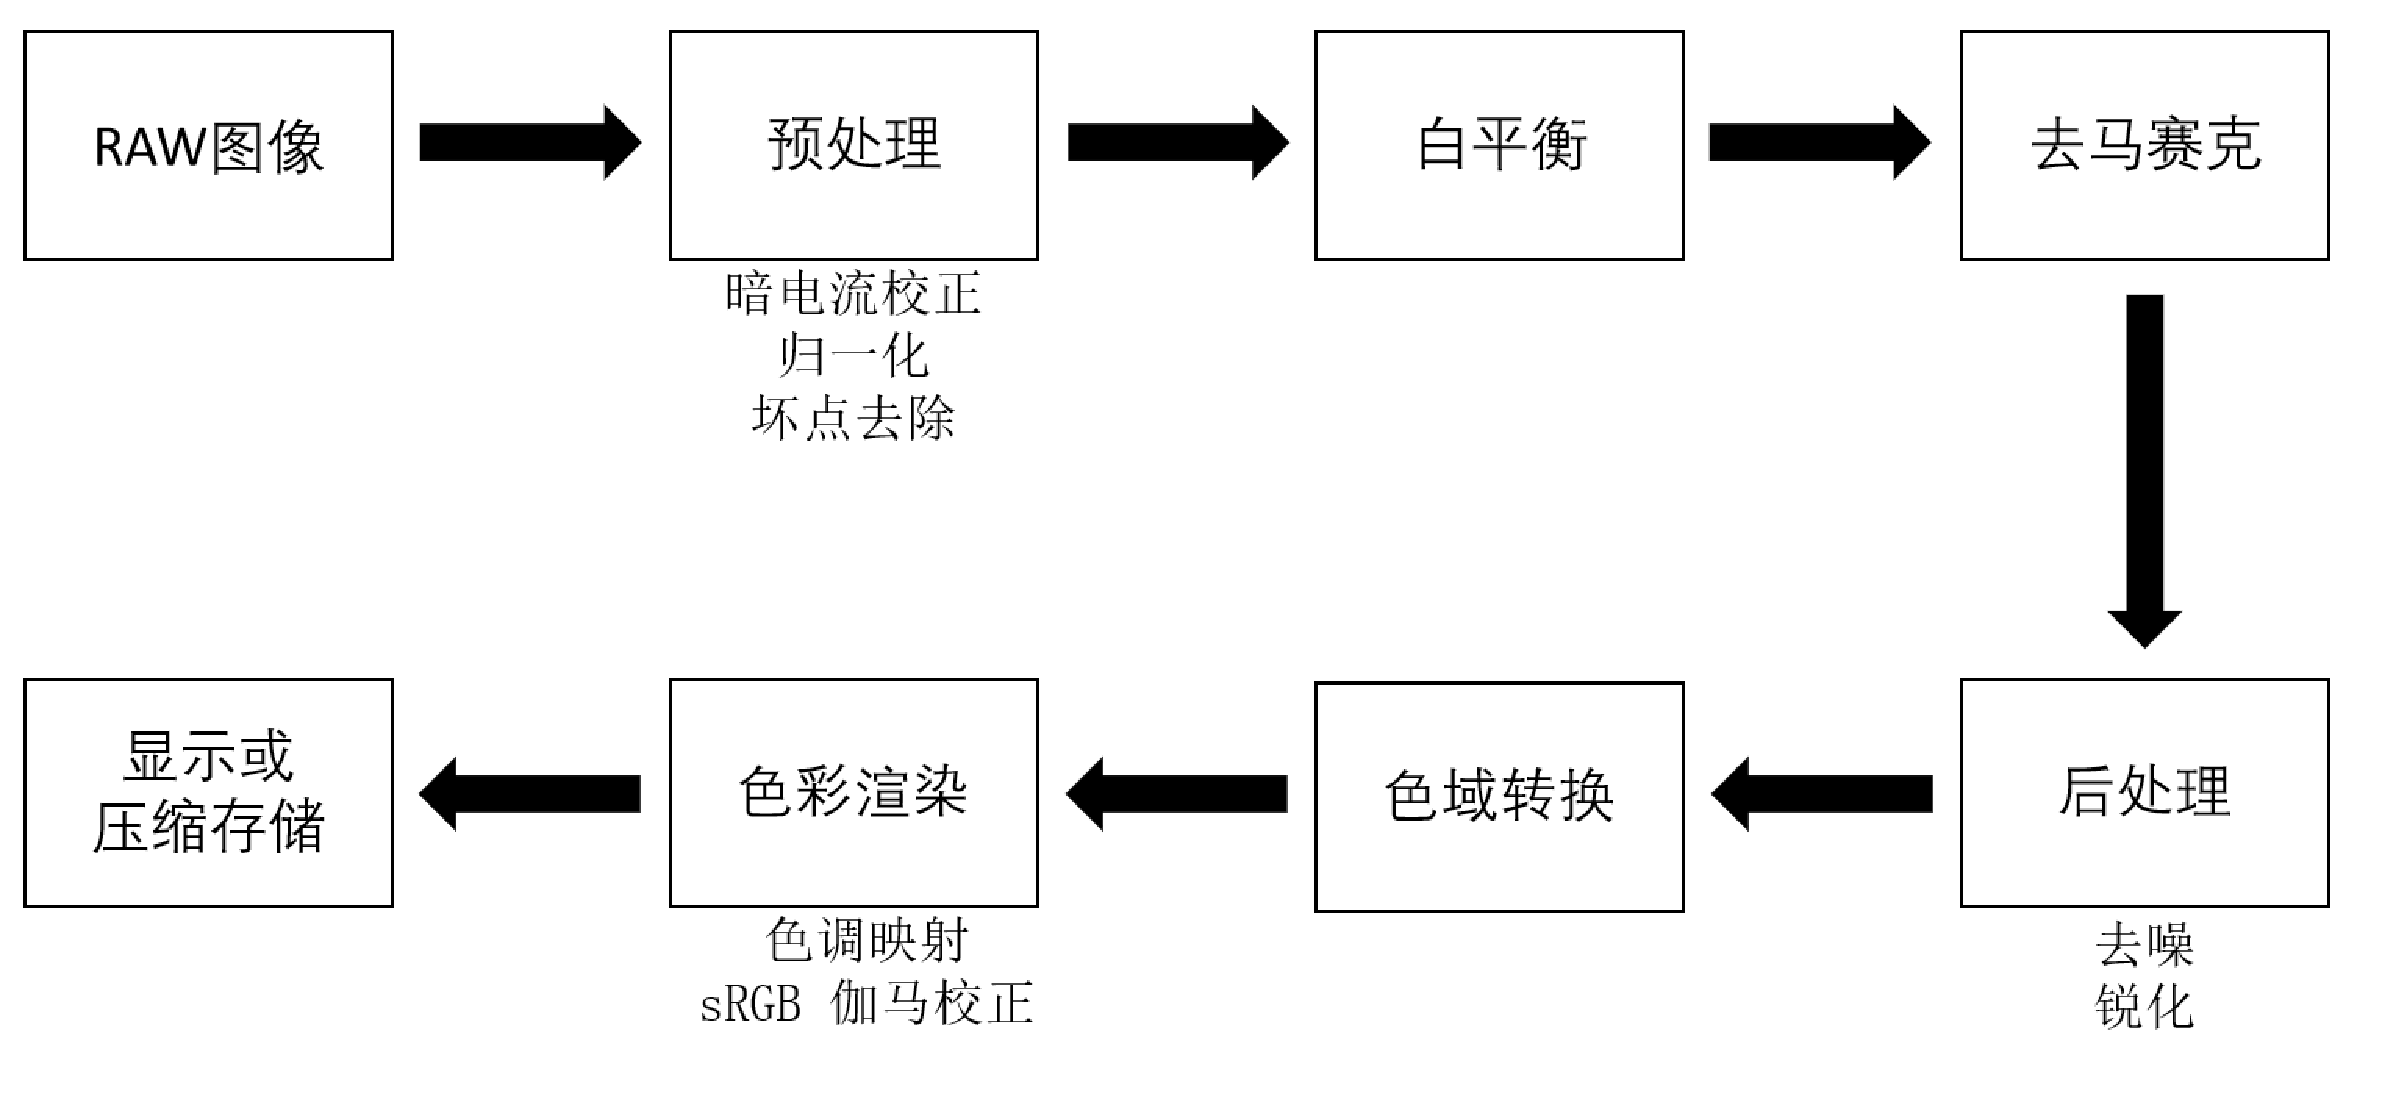
\includegraphics[width=1.0\linewidth]{docs/fig-chap3/fig-3-isp.pdf}
	\caption{图像处理流程图\quad 不同的相机硬件实现可能会有所不同,但是处理顺序类似}
	\label{fig:isp}
\end{figure*}

相机在生成全彩图像之前,需要先预处理从传感器获得的原始数据,去除噪点和伪影,一个常用的预处理步骤是缺陷像素校正,基本方法为通过对其邻域中准确记录的数据进行插值来估计缺陷位置的正确像素值。下一步是进行白平衡,校正在不同光源下引入的颜色偏差。在下一步进行去马赛克时,利用像素邻域信息来估计未测量的像素颜色,但这个过程会引入大量的预测值,就需要在后续的图像处理流程中进行去噪和锐化。人眼对尖锐的边缘高度敏感,且在水平和垂直方向的敏感度高于对角线方向,这也是许多相机厂商在进行图像锐化时会遵循的规律\cite{ramanath2005color}。相机与人眼对颜色的敏感度并不相同,相机在图像处理时需要将RGB值转换到更符合人眼视觉的色域空间。色彩渲染是为了图像显示而设计的,这个过程涉及动态范围压缩和色调映射,最常见的渲染空间是sRGB颜色空间\cite{international1999multimedia}。


本研究中的图像增强任务处于图像处理中色彩渲染这一环节,涉及高动态范围(High Dynamic Range, HDR)场景的色调范围调整。动态范围是图像中最大亮度与最小亮度的比值,大于$2^{16}$称为高动态范围,大于$2^{10}$称为增强动态范围(Enhanced Dynamic Range, EDR),小于等于$2^{10}$称为低动态范围(Low Dynamic Range, LDR)。通常将HDR图像和EDR图像统称为HDR图像,而常见的8位图像则是LDR图像\cite{han2023high}。受硬件限制,现有的技术不能使图像显示像真实场景一样具有大的动态范围,不经过任何处理而直接显示HDR图像将导致场景的暗区和亮区的细节丢失,通常可以用色调映射的方法解决这个问题。色调映射是一种在保持视觉效果基本不变的前提下将高动态范围图像映射到常规低动态显示设备上进行显示的技术\cite{朱仲杰2023宏微观信息增强与色彩校正的高效色调映射},目的是使得动态范围压缩后显示出的图像更符合人类视觉系统(Human Visual System, HVS)的感知。

色调映射常用的方法是直方图均衡化\cite{J21},从全局上提高整幅图像的对比度。然而,在处理高动态范围的场景时,全局操作往往会出现不足。在深度学习时代,基于颜色变换的方法通常以全局-局部协同的方式用于高分辨率图像的实时处理。根据获取颜色变换函数的不同方式,这些方法可以分为仿射变换矩阵\cite{J11,J33}、多层感知器(MultiLayer Perceptron, MLP)\cite{J14}、三维查找表(3D Look Up Table, 3D\;LUT)\cite{J35,J38,J40}等。开创性的工作是高动态范围网络(HDRNet)\cite{J11},它在低分辨率下学习系数的双边网格(Bilateral Grid),并在全分辨率下执行从输入到输出的转换,从而在不降低色调映射的效果的前提下提高算法的运行速度。自适应三维查找表\cite{J38}将仿射变换矩阵替换为图像自适应的三维查找表,实现了快速、鲁棒的图像增强。

在本章中,本文使用的高光谱相机的光谱响应范围包含可见光和近红外,利用近红外波段代表室外太阳光照在图像中不同局部的强度,从而跨模态地去除RGB图像中光源强度的影响,更好地引导RGB图像的增强。本文将高光谱图像中的近红外波段近似地看做是本征信息分解输出的光照信息并与RGB图像共享,提出了局部亮度适应法,在保证颜色不变的情况下将高动态范围图像各区域的亮度压缩到低动态范围的亮度,便于色调映射。本文选择HDRNet作为图像增强的基线,关键的挑战在于多模态信息的融合,包括将HDRNet与额外的低空间分辨率光谱图像集成。为此,本文提出了光谱感知自注意机制,将光源光谱嵌入到RGB特征图中,提升了RGB图像色调映射的效果,使得高动态范围图像压缩到低动态范围后仍保留丰富的色彩信息。

% \section{相关研究现状}

% 高光谱成像技术采用更多的通道从场景中捕获更多的光谱细节,并通过光源光谱标定和光谱反射率校正,使其在真实颜色复现中应用广泛。

% 在图像增强任务中有关色调映射的这一方面,分为全局和局部色调映射,具有全局映射函数的三维查找表以及具有局部映射函数的HDRNet中的双边网格都描述了简单的、可解释的色调映射规则,同时具有显著的图像增强效果。为此,我们将以三维查找表和HDRNet为色调映射研究的理论基础,分别展示图像增强色调映射的研究中,基于全局色调映射和基于局部色调映射的设计思路。

% \subsection{高动态范围网络}
% 高动态范围网络(HDRNet)\cite{J11}提出了一种新的卷积网络架构,可以实现端到端的训练,并已实现在现代智能手机上以高清视频级的速度实时运行。

% \begin{figure*}[h]
% 	\centering
% 	%\fbox{\rule{0pt}{2in} \rule{0.9\linewidth}{0pt}}
% 	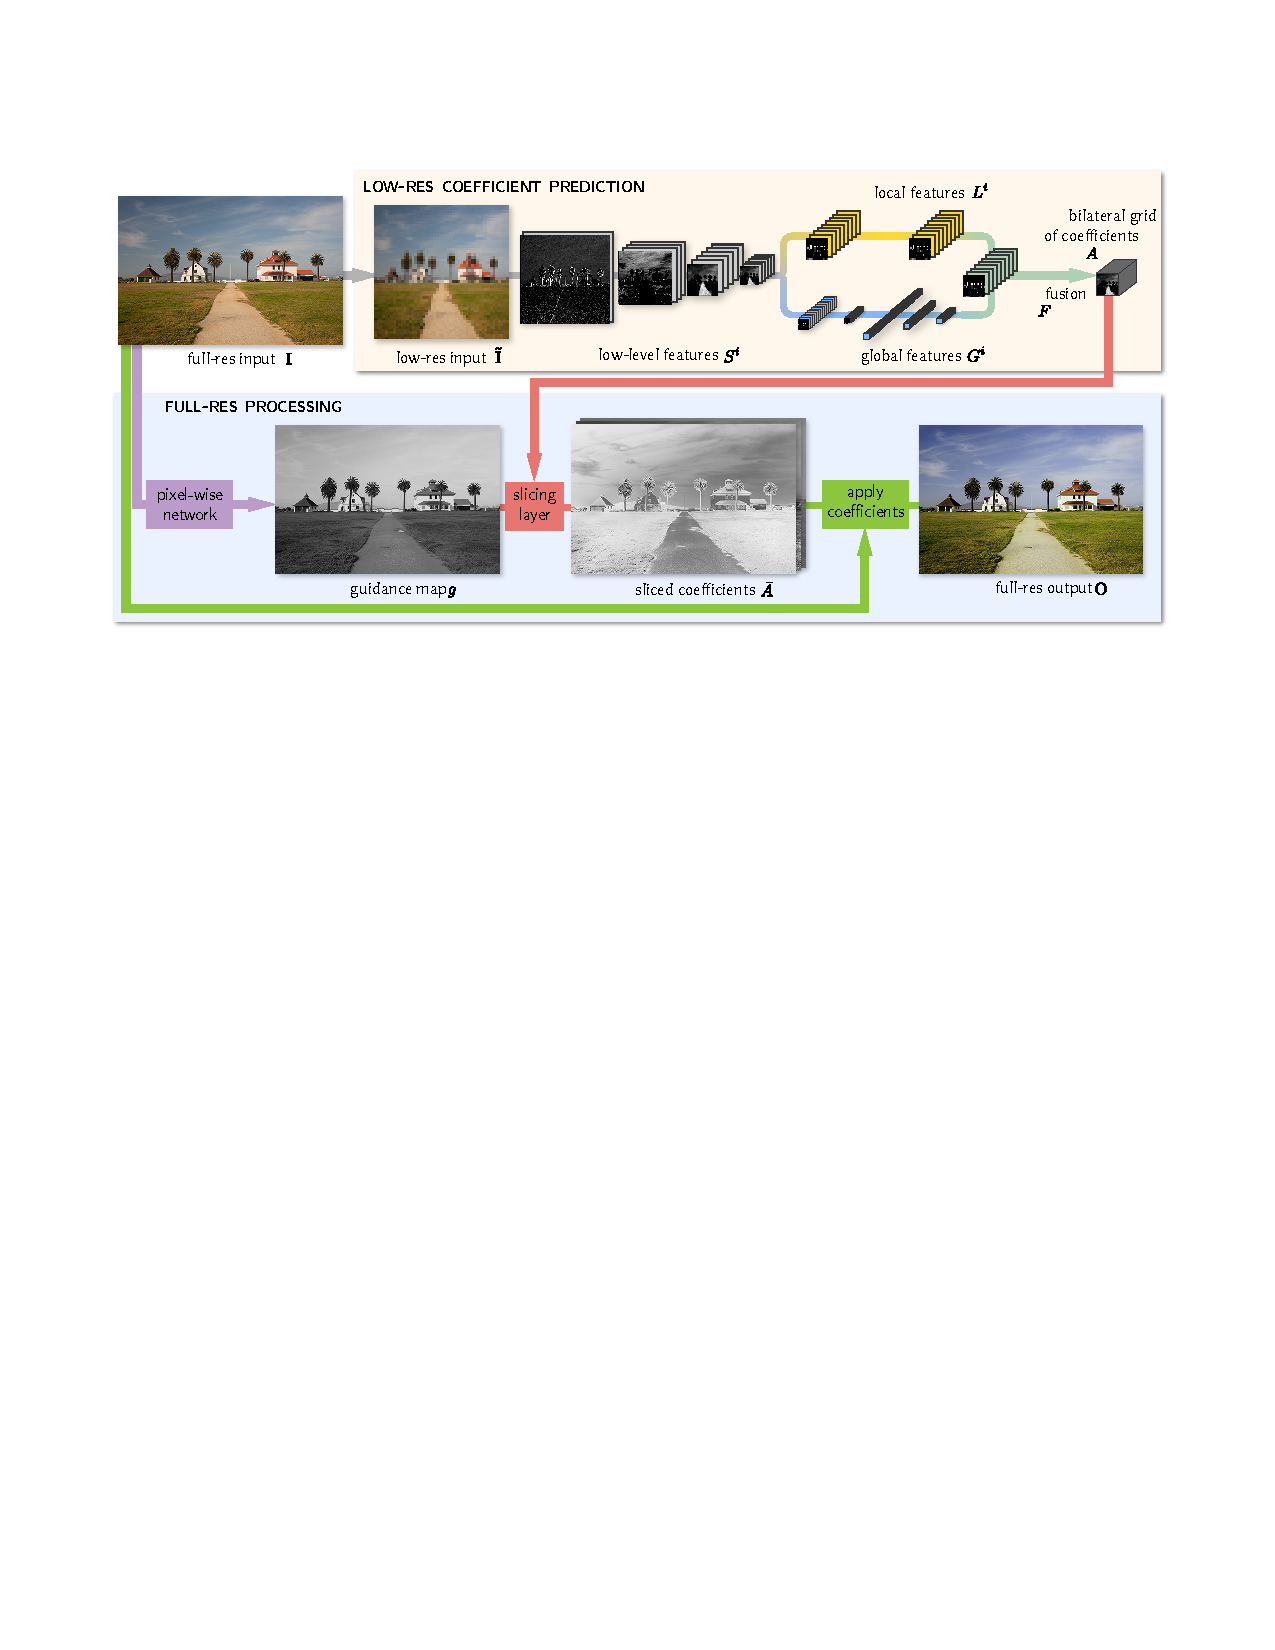
\includegraphics[width=1.0\linewidth]{docs/fig-chap3/fig-3-hdrnet.pdf}
% 	\caption{HDRNet的结构示意图\cite{J11}}
% 	\label{fig:hdrnet}
% \end{figure*}

% 如图\ref{fig:hdrnet}所示,HDRNet在低分辨率流中对输入图像的低分辨率版本进行了大部分推理,最终以类似于双边网格(Bilateral Grid)的表示方式预测了局部仿射变换。根据经验,图像增强通常不仅依赖于局部图像特征,还依赖于全局图像特征,如亮度直方图,平均强度,甚至场景类别。因此,HDRNet的低分辨率流被进一步分裂为局部路径和全局路径,然后,融合这两条路径,从而产生表示仿射变换的最终系数。

% 高分辨率流在全分辨率下工作,执行尽可能少的计算,但在捕获高频分量和在需要保留边缘时起到关键作用。为此,HDRNet引入了一个受双边网格处理启发的切片节点,该节点在基于学习的引导图的低分辨率网格中执行数据依赖的查找。给定用全分辨率引导图在网格中得到的高分辨率仿射系数,对每个像素应用局部颜色变换以产生最终输出。在训练时,在全分辨率下进行最小化损失函数的计算。这意味着,只处理大量低采样数据的低分辨率流,仍然可以学习中间特征和可以重现高频分量的仿射系数。

% 作为第一个近似,HDRNet的工作减轻了双边引导上采样中运行时对参考过滤器的需要。在某种意义上,HDRNet寻求预测仿射颜色变换系数在双边网格给定一个低分辨率版本的图像。然而,除此之外,还有几个关键元素。首先,学习对双边网格的下采样。第二,也学习了引导图,而不限于亮度。最后,将损失函数不应用于仿射系数上,而是应用于全分辨率的最终图像上,这允许HDRNet捕获图像高频分量并处理非尺度不变的算子。
%Husseis等人在此基础上提出了确定该权重值的自适应方法

\section{相关研究 }
\subsection{高动态范围图像的亮度调整}
高动态范围图像的亮度调整受人类视觉系统的启发,Drago等人\cite{TM6}对图像亮度的动态范围进行对数压缩,通过使用较小的对数底数来更好地增亮暗像素,并通过使用更大的对数底数来压缩较亮的像素。Kim等人\cite{TM7}在此基础上加入了非线性比例因子,更好地适配人眼视网膜的响应。Lee等人\cite{TM8}为了保留HDR图像中最暗和最亮区域的细节,提出了一种非对称的S型曲线进行亮度调整。

图像亮度直方图是用于调整图像亮度的常见的依据。Duan等人\cite{TM34}通过直方图均衡映射与线性映射的加权平均值来构造直方图,两个映射相互补充,以提供更好的亮度调整性能。出于人的视网膜在暗光条件下对亮度变化更敏感这一经验,Khan等人\cite{TM37}构造了非均匀的亮度直方图,较暗的像素值对应较窄的宽度。Lee等人\cite{TM9}将亮度值聚类为固定数量的组,对每一组亮度自适应地确定一个用于色调映射的参数。Oskarsson\cite{TM10}采用动态规划方法求解聚类问题的全局最优解,并提出了对HDR图像亮度值的聚类。Yao等人\cite{TM12}通过在亮度直方图上使用高斯混合模型(Gaussian Mixture Model, GMM),估计了HDR图像的暗、亮区域的高斯分布,分别对暗区域和亮区域用高斯分布确定的参数进行亮度调整。


\subsection{基于学习的色调映射}
色调映射的研究广泛应用了深度学习算法。Rana等人\cite{TM13}提出了一种生成对抗网络来对各种场景的HDR图片进行高分辨率的色调映射,但是需要耗费大量的计算资源和时间。为解决这一问题,Cao等人\cite{TM14}用低分辨率的图像进行训练,对高分辨率和低分辨率的色调映射分别提出了优化后的架构。Panetta等人\cite{TM15}引入了一个注意力引导模块来克服色调映射时的伪影问题,并使用大规模低光照图像数据集扩充了色调映射的训练集。此外,Goswami等人\cite{TM18}还将HDR图像按场景分类,并使用全卷积网络对图像进行语义分割,对于不同的类别单独学习色调映射。

由于真实配对的HDR-LDR色调映射图像对较少,半监督的方法也被应用于色调映射。Zhang等人\cite{TM16}在原有的由HDR-LDR图像对计算的损失函数上增加了其他两个仅由LDR图像计算的损失项,并利用未配对的LDR数据,使得训练时可以减少对配对的HDR-LDR数据的依赖。Guo等人\cite{TM17}则在损失函数中引入了基于客观的图像质量评估(Image Quality Assessment, IQA)指标的无监督项,进一步减少了色调映射对大规模数据集的依赖。


\section{本文构建的图像增强数据集}

为了支撑本文提出的图像增强算法,本文构建了高光谱与RGB图像的图像增强数据集。

\begin{figure*}[h]
	\centering
	%\fbox{\rule{0pt}{2in} \rule{0.9\linewidth}{0pt}}
	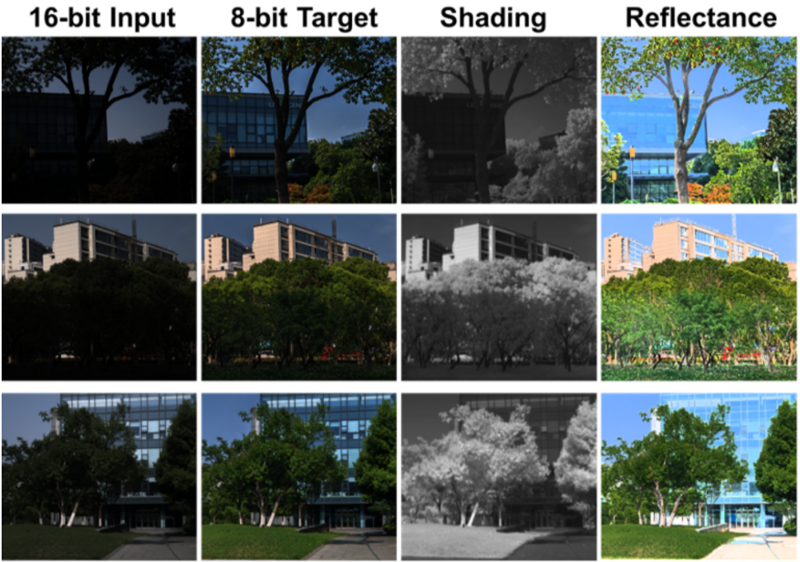
\includegraphics[width=1.0\linewidth]{docs/fig-chap3/fig-3-dataset.pdf}
	\caption{高光谱与RGB图像的图像增强数据集}
	\label{fig:enhance dataset}
\end{figure*}
据本文的调查,同时包含对齐的高光谱和RGB图像的图像增强数据集尚未被发现。为了弥补这一数据集缺口,本实验用智能手机和高光谱相机进行联合拍摄,构建了高质量的高光谱与RGB对齐的图像增强数据集,数据集包含200组图像,称为Mobile-Spec数据集。如图\ref{fig:enhance dataset}所示,每组图像同时具有16位RGB源图、8位RGB目标图、高光谱图像及其对应的阴影、反射率图像。

以上数据集面对的图像增强任务包含RGB图像动态范围压缩和色调映射,16位RGB图像作为图像增强的输入,8位RGB图像作为图像增强的输出。

% \subsection{数据筛选}

为了保证Mobile-Spec数据集的高质量,本数据集的数据经过了严格的筛选。首先,对16位源图仅保留了高动态范围样本,动态范围由图像中最大像素值和最小像素值之间的比值确定。其次,滤除了RGB与高光谱图像之间存在显著对齐误差的样本。第三,考虑色差、清晰度、噪声、伪影等因素,对8位目标图进行主观评价,剔除了视觉效果不理想的样本。最后,为了增加数据集内容的多样性,剔除了相似度高的场景。

% Mobile-Spec数据集的构建经过了

\subsection{双相机系统及其对齐}

% 为了解决智能手机上传感器光谱成像能力有限的问题,
本文构建的Mobile-Spec数据集是用高端商用智能手机和推扫式高光谱相机组成的双相机系统采集的。该推扫式高光谱相机的光谱范围为400-1000 nm,包含176个光谱通道。16位源图是智能手机图像处理过程中多个曝光帧的融合,8位目标图代表相应的色调映射结果。智能手机和推扫式高光谱相机在进行数据采集时,处于尽可能相近的位置,并使用三脚架进行固定,在使用高光谱相机推扫拍摄的过程中同步完成智能手机的拍摄。

% \subsection{图像匹配}

\begin{figure*}[h]
	\centering
	%\fbox{\rule{0pt}{2in} \rule{0.9\linewidth}{0pt}}
	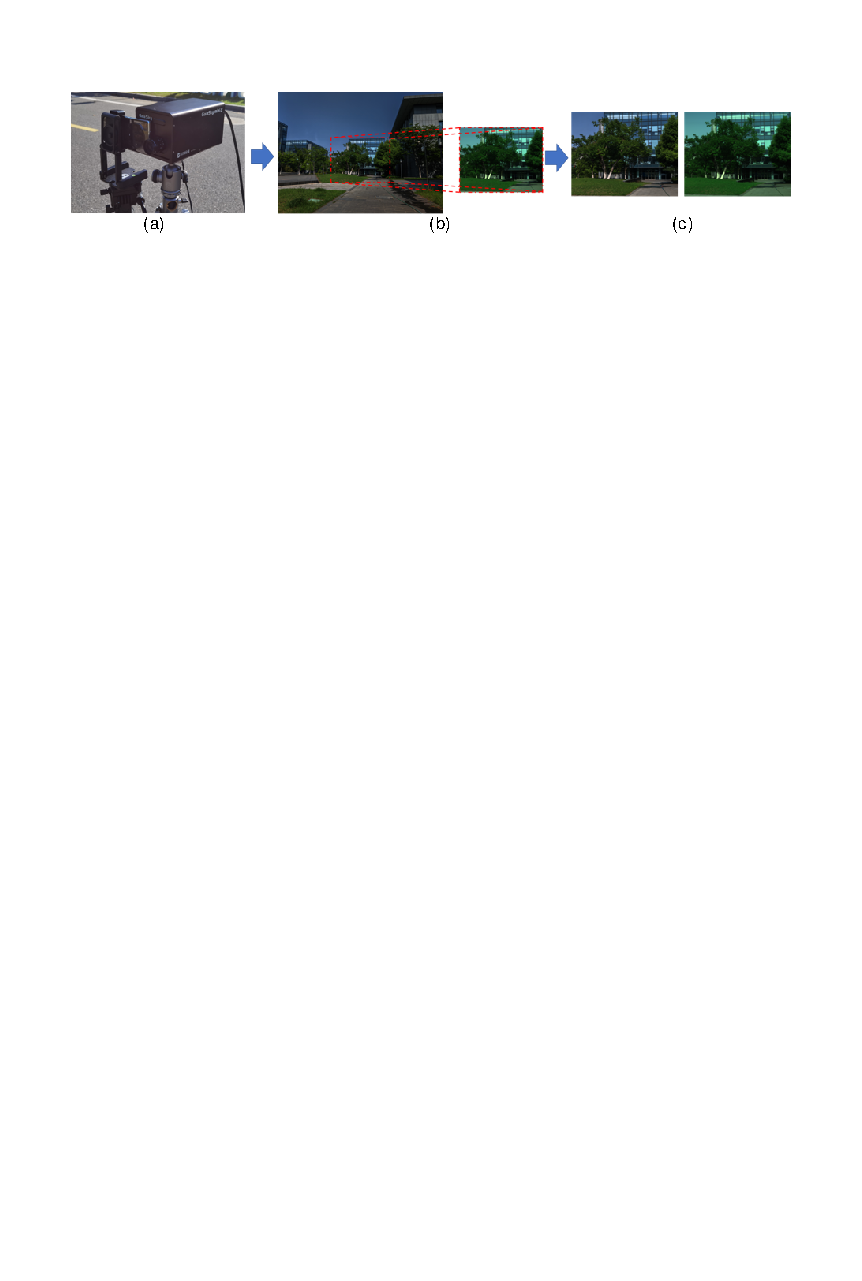
\includegraphics[width=1.0\linewidth]{docs/fig-chap3/fig-3-align.pdf}
	\caption{双相机系统的配准过程\quad (a)包括智能手机和高光谱相机的双相机系统\quad (b)RGB图像与高光谱图像的重叠区域由SIFT\cite{J25}算法检测得到,对智能手机捕获的RGB图像进行仿射变换,使之与高光谱图像渲染出的RGB图像对齐 \quad (c)对齐后的RGB和高光谱图像,其中高光谱图像被渲染为RGB形式}
	\label{fig:enhance align}
\end{figure*}

本实验采集到的高光谱图像分辨率为1057\times960\times176,16位源图、8位目标图的分辨率均为4096\times3072\times3。值得注意的是,高光谱图像与RGB图像在视场上存在相当大的差异。如图\ref{fig:enhance align}所示,为了将具有宽视角的RGB图像对齐到高光谱图像上,本文采用了一种自动的对齐算法,其中包括尺度不变特征变换(Scale Invariant Feature Transform, SIFT)\cite{J25}和估计最优的投影变换(Projective Transformation)算法。经过上述自动对齐算法,本实验将RGB图像对齐到高光谱图像上,使两种图像的空间分辨率均为1057\times960。

\subsection{光源的影响及阴影图}

如图\ref{fig:sun led}所示,阳光在可见光范围内包含连续的宽谱,延伸到紫外(UltraViolet, UV)和红外(InfraRed, IR)区域,其强度在可见光光谱中相对均匀。相反,LED光源的光谱特征是在蓝色区域有一个明显的峰值,其强度在近红外波长处迅速减弱。
\begin{figure*}[h]
	\centering
	%\fbox{\rule{0pt}{2in} \rule{0.9\linewidth}{0pt}}
	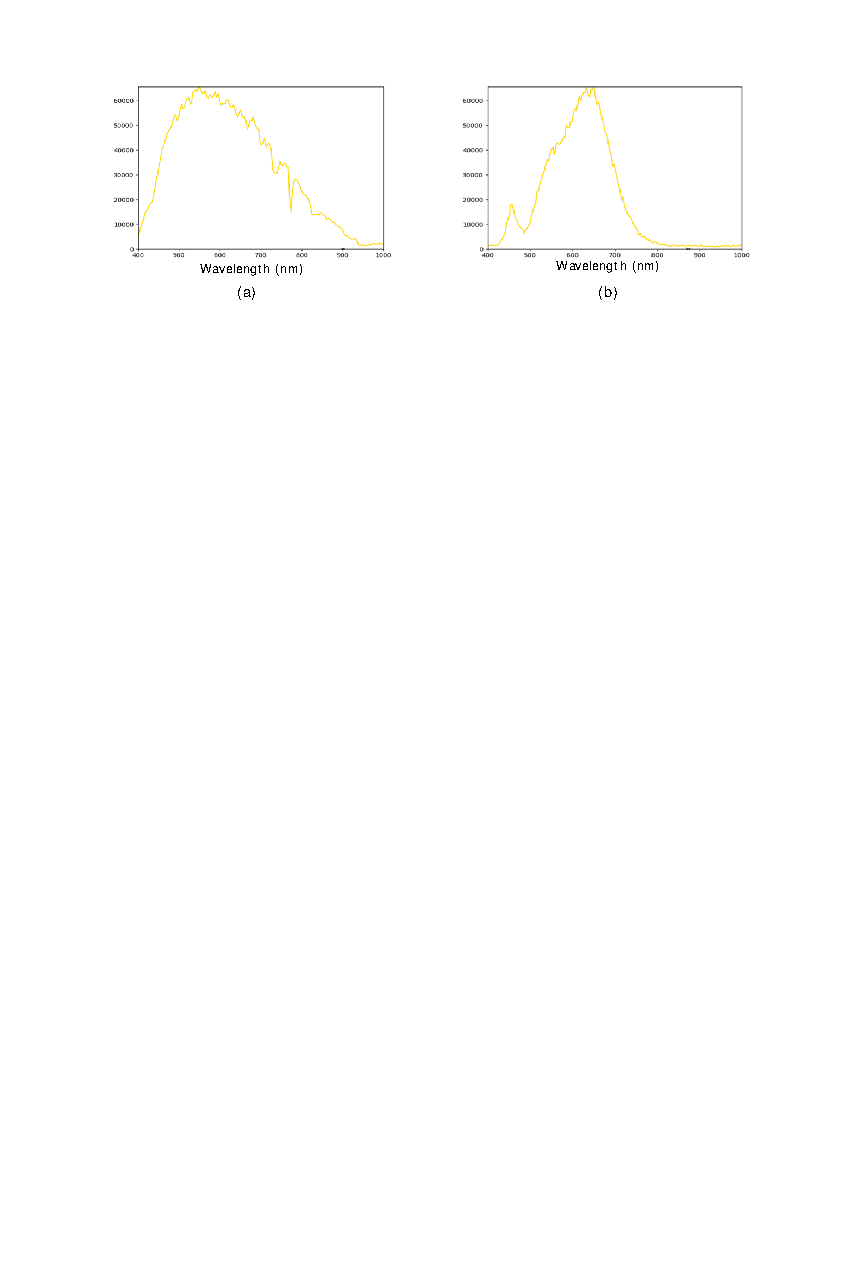
\includegraphics[width=1.0\linewidth]{docs/fig-chap3/fig-3-sun-led.pdf}
	\caption{室外光与室内光的光谱区别\quad (a)太阳光光谱曲线 \quad (b)LED光源光谱曲线}
	\label{fig:sun led}
\end{figure*}

如图\ref{fig:enhance category curve},可以发现,不同的材质在太阳光下的近红外反射强度是接近的,可以近似地认为,高光谱图像中近红外部分只反映太阳光的强度,而可见光部分则反映颜色。
\begin{figure*}[h]
	\centering
	%\fbox{\rule{0pt}{2in} \rule{0.9\linewidth}{0pt}}
	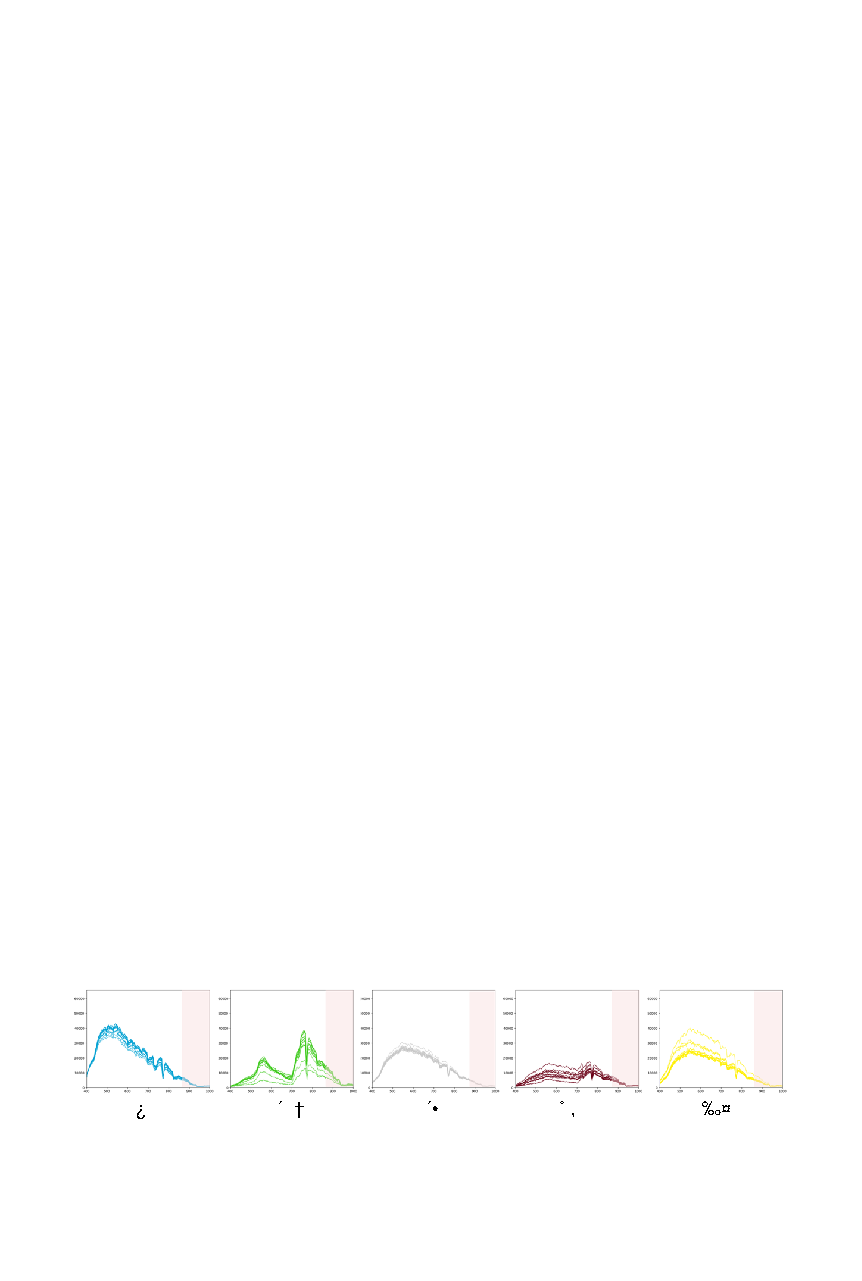
\includegraphics[width=1.0\linewidth]{docs/fig-chap3/fig-3-category-curve.pdf}
	\caption{不同材质种类在太阳光下的光谱曲线,其中近红外波段表现出一致的趋势}
	\label{fig:enhance category curve}
\end{figure*}

\begin{figure*}[h]
	\centering
	%\fbox{\rule{0pt}{2in} \rule{0.9\linewidth}{0pt}}
	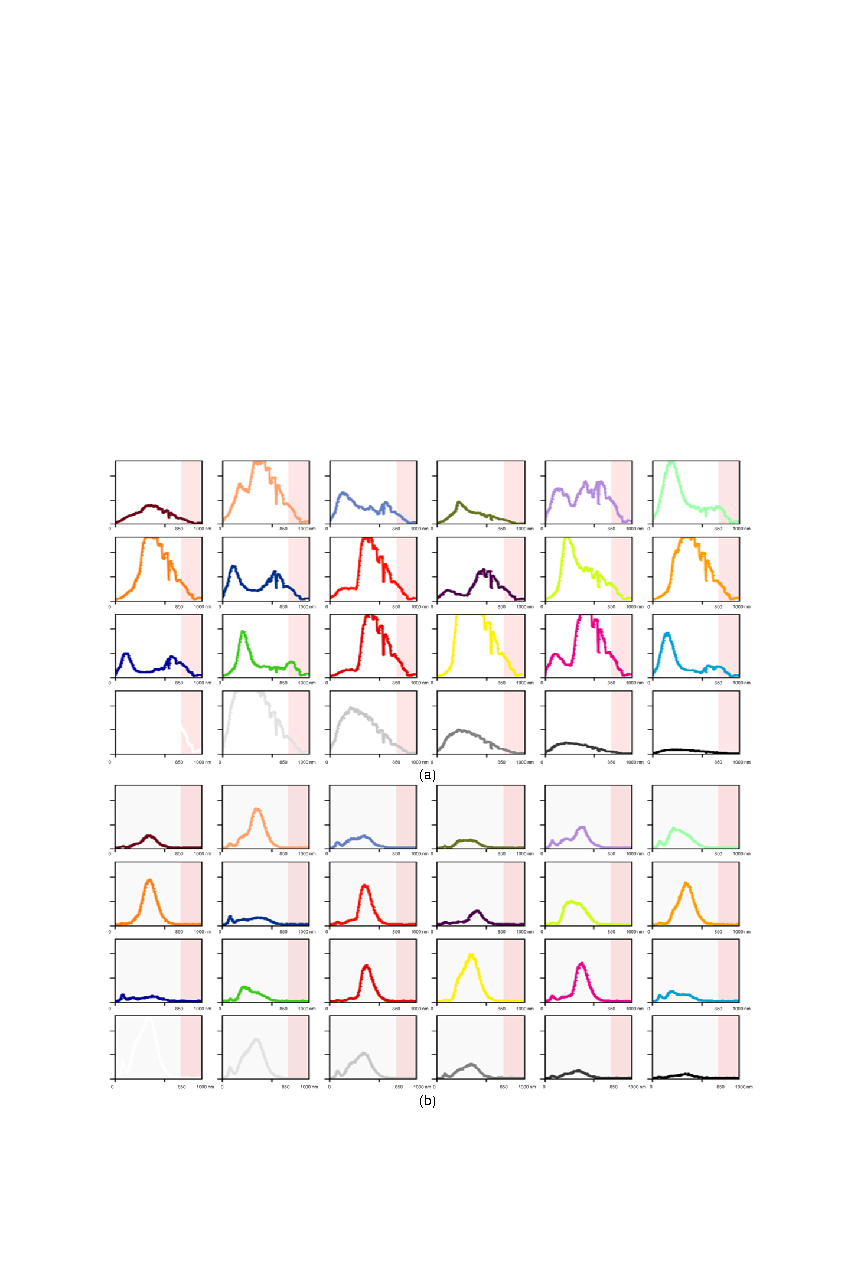
\includegraphics[width=1.0\linewidth]{docs/fig-chap3/fig-3-colorchecker-curve.pdf}
	\caption{24色标准色卡的每个颜色在不同光源下的光谱曲线,其中标红的区域为近红外波段中850-1000nm的部分\quad (a)室外太阳光 \quad (b)室内LED光源}
	\label{fig:colorchekcer curve}
\end{figure*}

\begin{figure*}[h]
	\centering
	%\fbox{\rule{0pt}{2in} \rule{0.9\linewidth}{0pt}}
	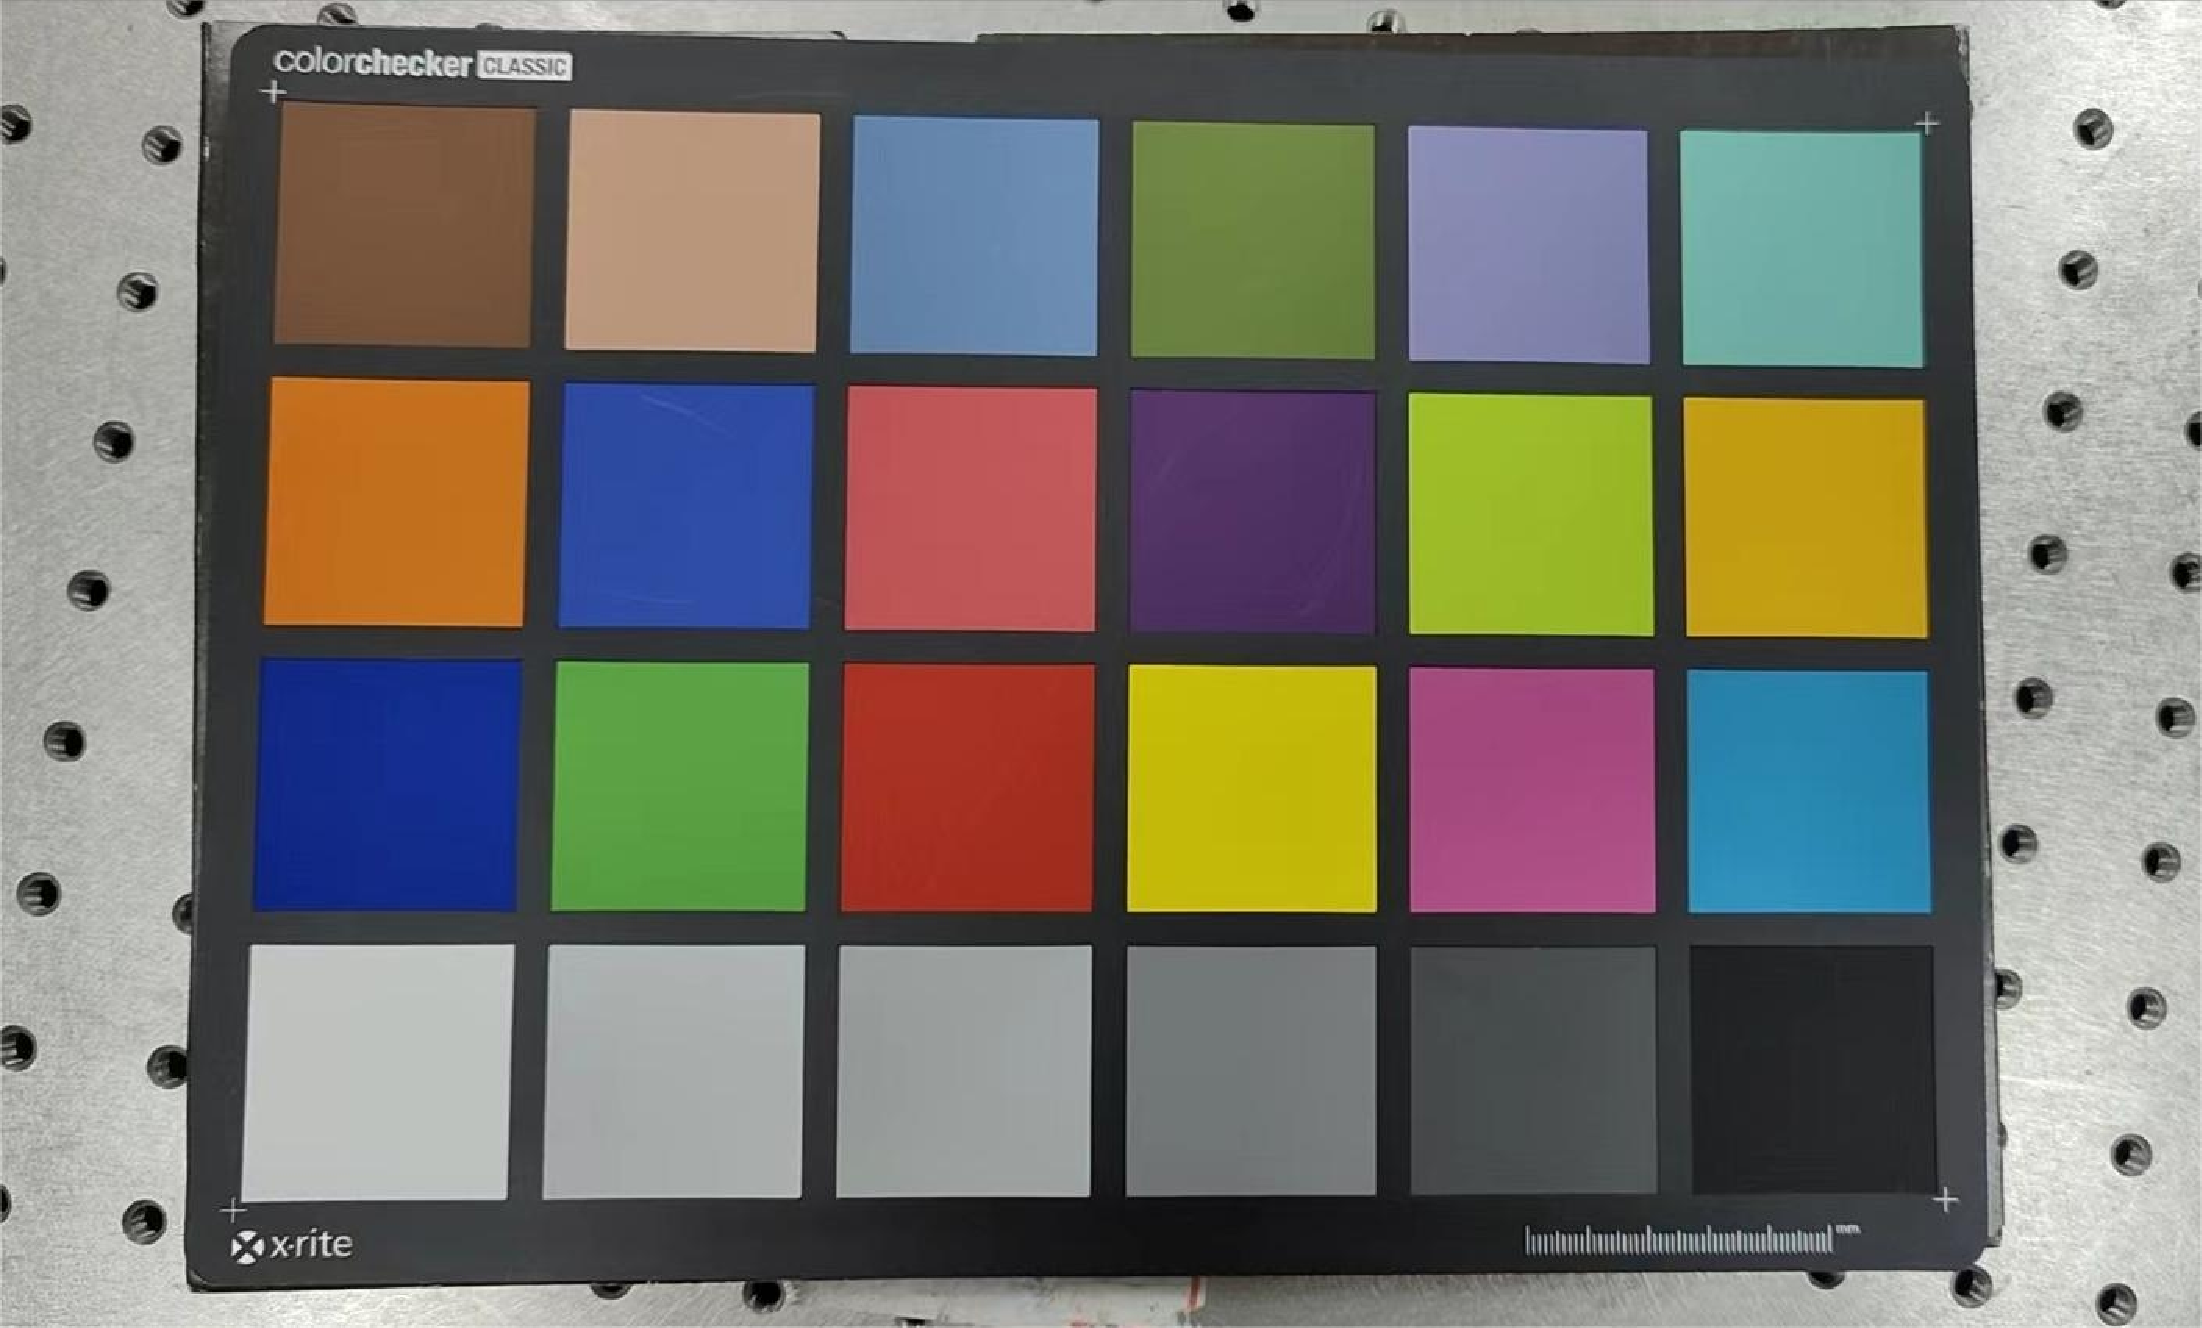
\includegraphics[width=1.0\linewidth]{docs/fig-chap3/fig-3-colorchecker.pdf}
	\caption{实验用到的24色标准色卡}
	\label{fig:colorchekcer}
\end{figure*}

进一步地,本文在24色标准色卡(如图\ref{fig:colorchekcer})上测试各种颜色在室内和室外光下的光谱曲线,图\ref{fig:colorchekcer curve}(a)反映出在太阳光下各种颜色在近红外波段同样表现出类似的趋势,而图\ref{fig:colorchekcer curve}(b)则表明在LED光源下各种颜色的近红外波段响应几乎为零。
% \subsection{阴影图和反射率图}

因此,近红外图像包含亮度信息且不包含可见光颜色信息,可以充当阴影图\cite{J7},本实验通过对高光谱图像中850nm到1000nm的近红外波段进行平均来逼近阴影图。基于Retinex理论\cite{J3,J22},使用采集到的高光谱图像除以阴影图得到反射率图。

这样,本文就解决了真实阴影图难以获取的问题,从而避免使用算法进行本征分解,而是使用更可靠的直接测量的方法来获得阴影图。

为了利用太阳光在近红外的辐射以获得高质量的阴影图,并避免复杂的室内光源对数据集采集的不利影响,本文将Mobile-Spec数据集的采集场景限制在室外。
% 假设。数据集收集。我们的数据集跨越多个季节,包括春季、夏季和秋季。

% 因此,近红外图像包含亮度信息且不包含可见光颜色信息,可以充当阴影图\cite{J7},我们通过对高光谱图像中850nm到1000nm的近红外波段进行平均来逼近阴影图。基于Retinex理论\cite{J3,J22},使用采集到的高光谱图像除以阴影图得到反射率图。

% 这样,我们就解决了真实阴影图难以获取的问题,从而避免使用算法进行本征分解,而是使用更可靠的直接测量的方法来获得阴影图。

% 为了利用太阳光在近红外的辐射以获得高质量的阴影图,并避免复杂的室内光源对数据集采集的不利影响,我们将Mobile-Spec数据集的采集场景限制在室外。

\section{本文提出的方法}
在HDRNet\cite{J11}的研究基础上,本文提出了局部亮度适应来调整高动态范围RGB图像不同区域的亮度,并提出光谱感知自注意机制,将光源光谱嵌入到RGB图像增强的特征图中,提高色调映射的效果。


\begin{figure*}[h]
	\centering
	%\fbox{\rule{0pt}{2in} \rule{0.9\linewidth}{0pt}}
	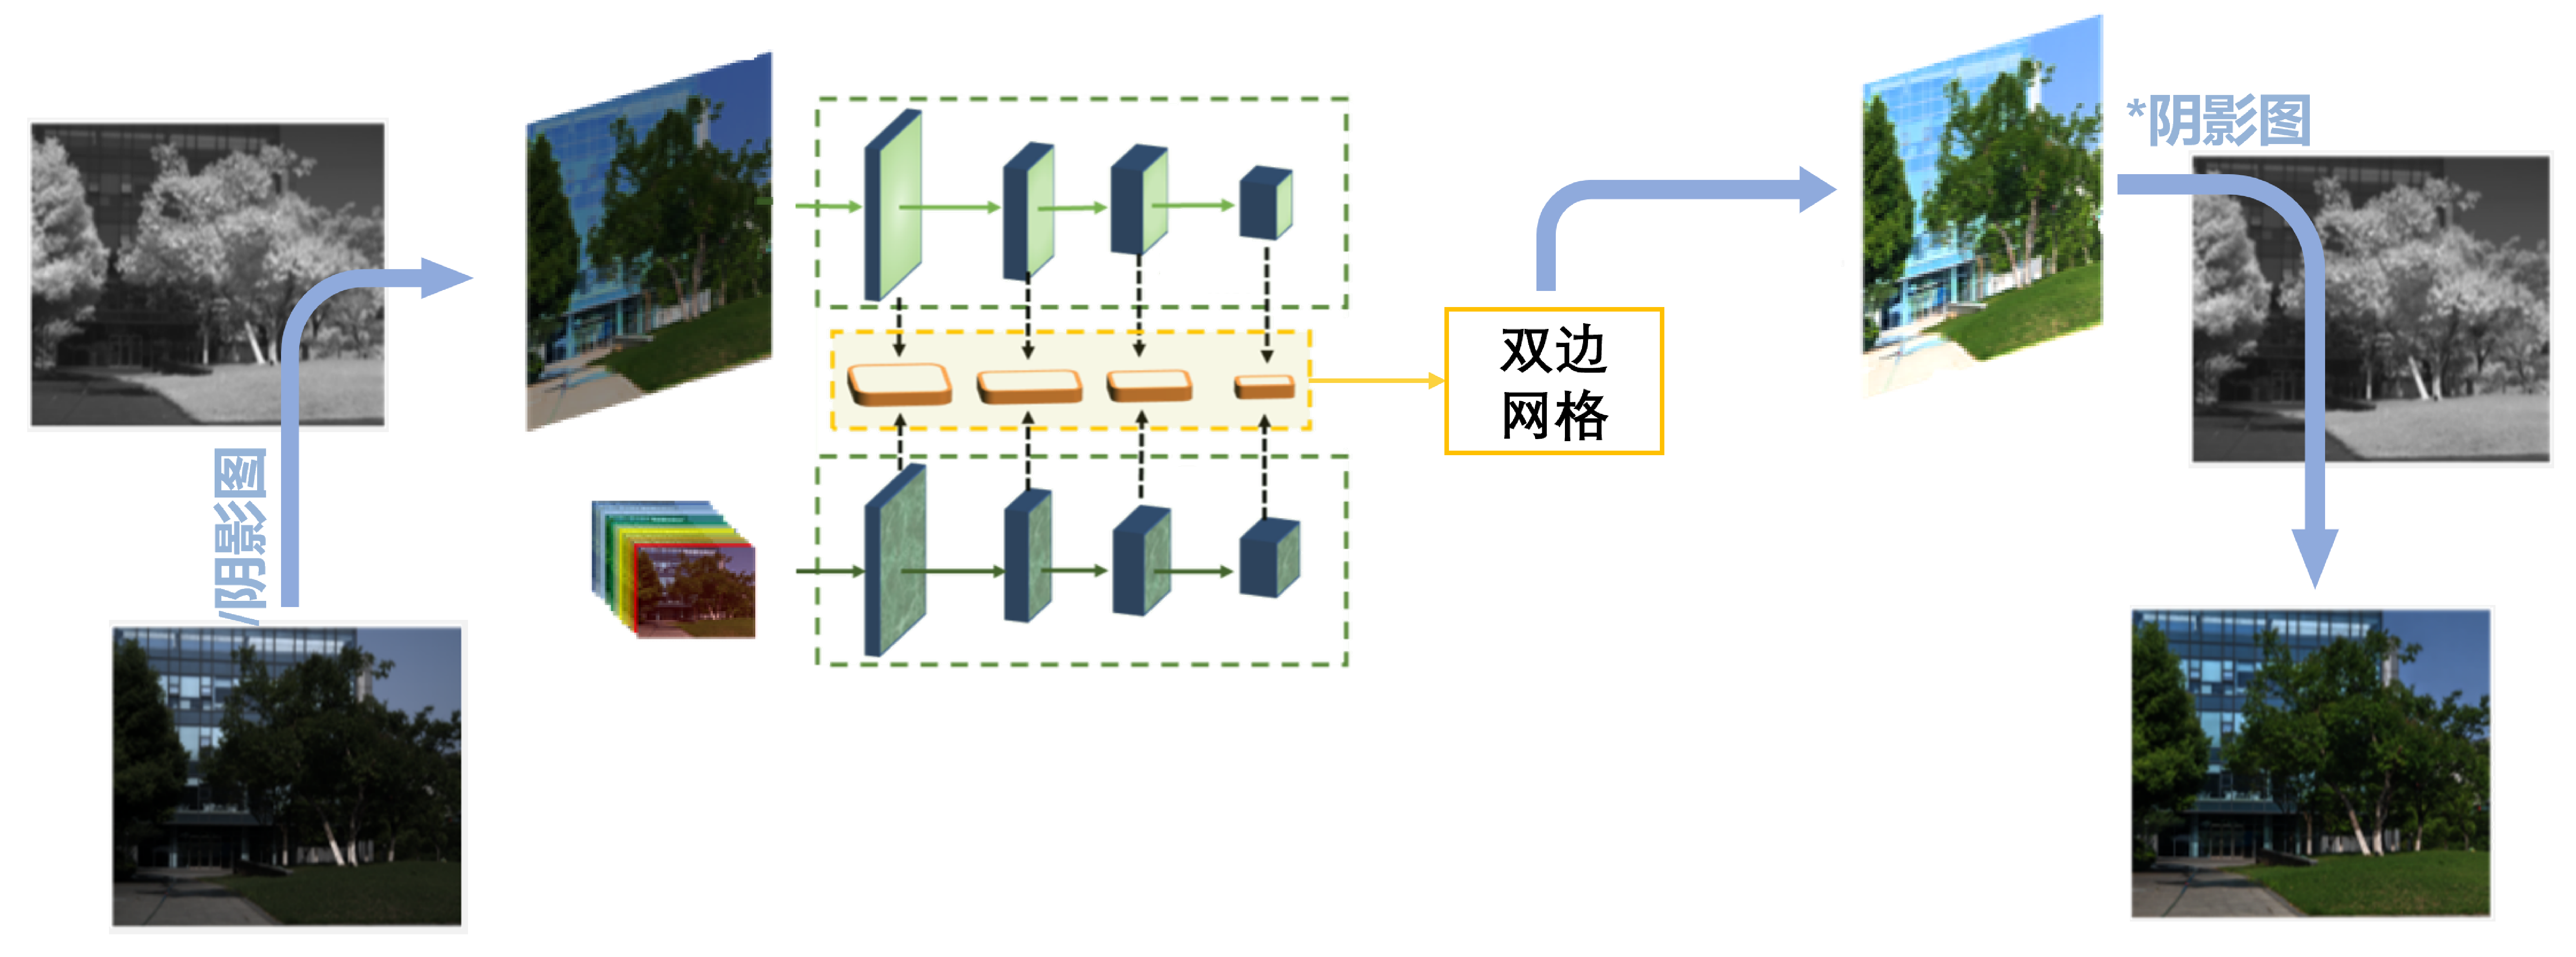
\includegraphics[width=1.0\linewidth]{docs/fig-chap3/fig-3-pipeline.pdf}
	\caption{本文提出的图像增强方法示意图}
	\label{fig:enhance pipeline}
\end{figure*}

本文提出的图像增强方法示意图如图\ref{fig:enhance pipeline}所示,本文参考HDRNet的方法进行图像增强,训练了一个双边网格用于色调映射。其中,代表光源强度的阴影图不参与色调映射过程,称为阴影先验。将额外引入的低分辨率光谱反射率图作为反射率先验,进一步引导双边网格的训练。浅蓝色箭头表示主要的图像处理流程,“/阴影图”表示使用逐像素的除法去除阴影图得到反射率图,“*阴影图”表示使用逐像素的乘法将阴影图重新叠加到反射率图上,从而得到最终的图像增强结果。



\subsection{局部亮度适应}

\begin{figure*}[h]
	\centering
	%\fbox{\rule{0pt}{2in} \rule{0.9\linewidth}{0pt}}
	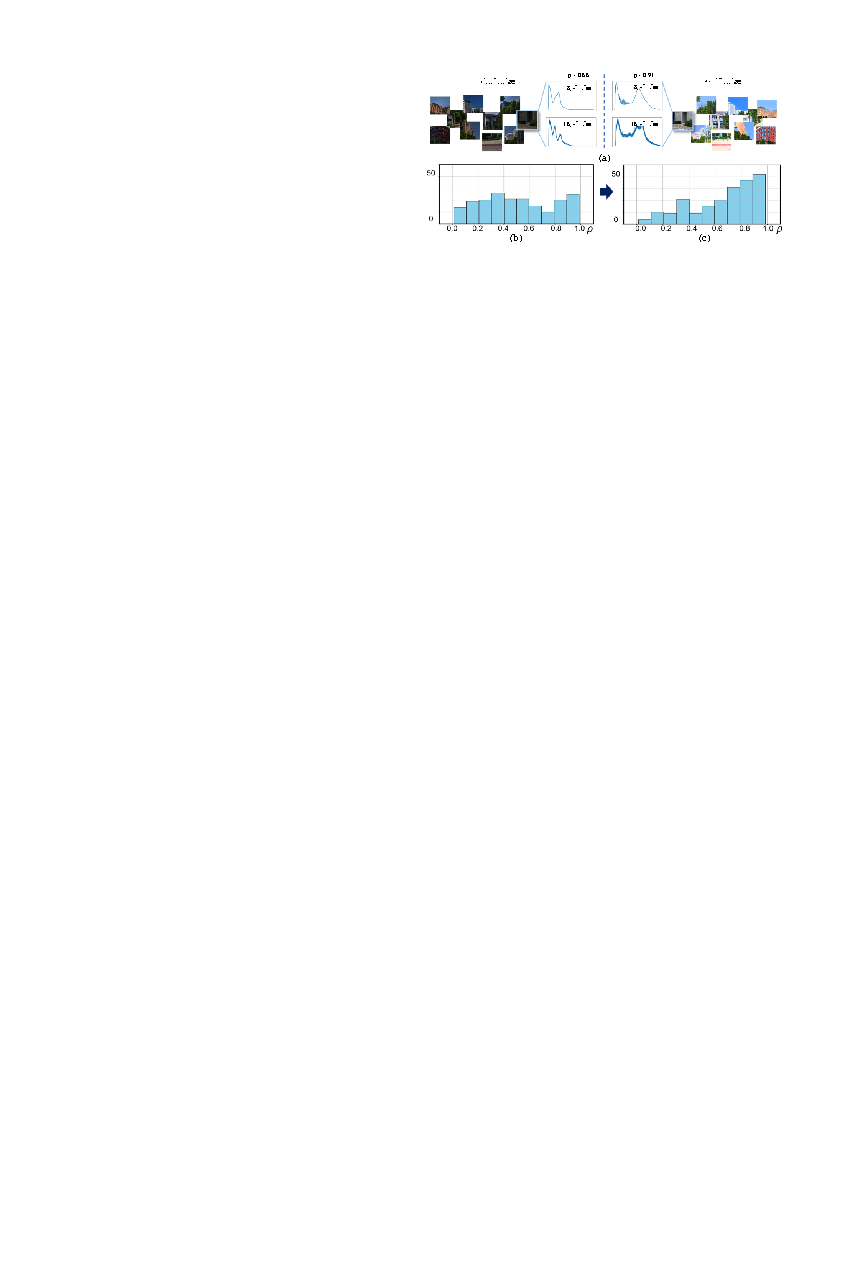
\includegraphics[width=1.0\linewidth]{docs/fig-chap3/fig-3-reflectance.pdf}
	\caption{局部亮度适应的作用\quad (a)一对原始图像和反射率图像的亮度分布统计\quad (b)(c)8位图像与对应的16位图像的亮度分布的皮尔逊相关系数(Pearson correlation coefficient)$ρ$在原始图像集和反射率图像集中的直方图}
	\label{fig:enhance reflectance}
\end{figure*}
为了在色调增强过程中同时对高亮区域和阴影区域进行调整,HDRNet中的双边网格深度设置为8,可以容纳8种不同的亮度级别。然而,这种设计在处理高动态范围场景中的各种局部亮度变化时可能不具有足够的适应性。

本文认为,在这种情况下,去除阴影分量会简化色调映射过程,为模型的学习带来好处。如图\ref{fig:enhance reflectance} (a)所示,16位输入和8位目标之间的像素值分布向量在原始图像中表现出0.66的皮尔逊相关系数$ρ$,在反射率图像中增加到0.91。系数$ρ$越大,表示16位图像与8位图像的亮度特征相似度越大,相互间的映射关系也就越简单。通过对Mobile-Spec数据集中$ρ$分布的统计发现,与原始图像集(图\ref{fig:enhance reflectance} (b))相比,反射率图像集(图\ref{fig:enhance reflectance} (c))具有更大比例的高$ρ$样本。

这一现象表明,将原始图像中的阴影分量去除,得到反射率图像后,可能会降低颜色映射学习的难度。

在本文提出的方法中,为了将阴影分量$S$转换为具有8个亮度等级的亮度图$\hat{S}$,本文提出了一个局部亮度自适应模块,包含两层卷积和反卷积。该轻量级模块将缓解局部高动态范围区域亮度的剧烈变化,从而进一步增强自适应性。

通过以下等式可以将图像中各个局部不同的光源强度去除:
\begin{equation}
\begin{aligned}
R_{r g b}=I_{r g b} / \hat{S}, \\
R_{hsi}=I_{hsi} / \hat{S}.
\end{aligned}
\end{equation}

其中,$I_{r g b}$和$I_{hsi}$分别为输入的16位RGB图像和低空间分辨率的高光谱图像,$R_{r g b}$和$R_{hsi}$分别为去除光源强度后的对应的反射率图像。

随后,16位图像的反射率图像$R_{r g b}$和低空间分辨率光谱图像的反射率图像$R_{hsi}$将被送入双边网格的系数预测部分,用于预测图像增强的颜色变换系数。



\subsection{光谱感知自注意}
从原始图像转换到反射率图像后,本文利用低空间分辨率光谱图像的反射率图像$R_{hsi}$来增强双边网格的颜色映射学习。

本文认为,由于双边网格系数的预测是在更低的空间分辨率下进行的,因此,在空间维度上的下采样不会给颜色映射造成明显的退化。由此,本文设计了光谱感知自注意(Spectral Perception Self-Attention, SPSA)模块,利用$R_{hsi}$引导$R_{rgb}$在颜色映射学习中产生更好的双边系数。$R_{hsi}$与$R_{rgb}$在空间分辨率上相互配准,均为256\times256,用于HDRNet中的低分辨率双边网格的系数预测。

SPSA模块对$R_{hsi}$和$R_{rgb}$进行卷积层堆叠处理,生成分层特征图。将这些特征图$\mathcal{F}_{R_{msi}}$、$\mathcal{F}_{R_{rgb}}$沿通道维拼接,形成交叉谱特征图$\mathcal{F}_{R}$。然后将1\times1卷积$W_1$和3\times3深度卷积$W_3$应用到$\mathcal{F}_{R}$中生成查询$Q$、密钥$K$和值$V$:

\begin{equation}
\begin{align}
Q=W_1^Q W_3^Q \mathcal{F}_{\mathcal{R}},\\
K=W_1^K W_3^K \mathcal{F}_{\mathcal{R}},\\
V=W_1^V W_3^V \mathcal{F}_{\mathcal{R}}.
\end{align}
\end{equation}

$K$和$Q$被重塑为$\hat{K} \in \mathbb{R}^{C \times HW}$和$\hat{Q} \in \mathbb{R}^{H W \times C}$,它们的点积交互产生了光谱通道间的自注意$A \in \mathbb{R}^{C \times C}$。光谱感知自注意$A$对重构$\hat{V} \in \mathbb{R}^{H W \times C}$的不同通道的重要性进行了重新加权。将卷积$W_3$沿通道维度拆分为${W}_3^{hsi}$和${W}_3^{r g b}$,对应于$\mathcal{F}_{R_{msi}}$和$\mathcal{F}_{R_{rgb}}$的通道,然后重塑为$\hat{W}_3^{hsi}$和$\hat{W}_3^{r g b}$以适应$\hat{V} \cdot A$的形状。最终,SPSA模块可表示为:
\begin{equation}
\begin{aligned}
A & =\operatorname{softmax}(\sigma \hat{K} \cdot \hat{Q}), \\
\hat{\mathcal{F}}_{R_{hsi}} & =\hat{W}_3^{hsi} \hat{V} \cdot A+W_3^{hsi} \mathcal{F}_{R_{hsi}}, \\
\hat{\mathcal{F}}_{R_{r g b}} & =\hat{W}_3^{r g b} \hat{V} \cdot A+W_3^{r g b} \mathcal{F}_{R_{r g b}}.
\end{aligned}
\end{equation}

$σ$是一个可学习的缩放参数,用来控制$\hat{K}$与$\hat{Q}$点积的大小。SPSA模块作为残差学习,通过自适应的方式将交叉谱特征$\hat{V} \cdot A$与原始特征$\mathcal{F}_{R_{hsi}}, \mathcal{F}_{R_{r g b}}$进行加权融合。 SPSA模块的融合输出$\hat{\mathcal{F}}_{R_{hsi}}, \hat{\mathcal{F}}_{R_{r g b}}$以递进的方式馈入下一层。

\section{实验过程与结果分析}
在本章研究中,实验设置所使用的硬件平台和相关软件同第二章实验设置部分。

在Mobile-Spec数据集中,80\%的样本分配给训练集,剩下的20\%分配给测试集,批大小(Batch Size)为4,学习率为0.0001。网络参数的优化是通过最小化L2损失来实现的。在训练过程中,输入图像从1057\times960被裁剪为512\times512大小,这些图像在低分辨率流中被进一步下采样为256\times256。
\subsection{评价指标}
本文采用峰值信噪比(Peak Signal-to-Noise Ratio, PSNR)、结构相似性(Structural SIMilarity, SSIM)\cite{J34}和色差$\Delta E^*$共3个指标来验证图像增强方法的有效性。

图像增强的结果与目标图计算出的PSNR越大,表示图像增强的效果越好。对于空间分辨率为$m\times n$的两幅图像$I(i, j)$和$K(i, j)$,PSNR的计算方式如下所示:
\begin{equation}
\begin{align}
M S E&=\frac{1}{m n} \sum_{i=0}^{m-1} \sum_{j=0}^{n-1}[I(i, j)-K(i, j)]^2 ,\\
P S N R&=10 \cdot \log _{10}\left(\frac{M A X_I^2}{M S E}\right)=20 \cdot \log _{10}\left(\frac{M A X_I}{\sqrt{M S E}}\right).
\end{align}
\end{equation}

其中$MAX_I$为图像可能的最大像素值,对于8位图像则为255。

SSIM对样本$x$和$y$的三个方面的相似性进行比较:亮度(luminance)\enspace $l(x, y)$、对比度(contrast)\enspace $c(x, y)$和结构(structure)\enspace $s(x, y)$,SSIM值越大表示样本间的相似度越高,计算方式如下:

\begin{equation}\label{lsc}
\begin{align*}
l(x, y)&=\frac{2 \mu_x \mu_y+c_1}{\mu_x^2+\mu_y^2+c_1}, \\
c(x, y)&=\frac{2 \sigma_x \sigma_y+c_2}{\sigma_x^2+\sigma_y^2+c_2}, \\
s(x, y)&=\frac{\sigma_{x y}+c_3}{\rho_x \sigma_y+c_3} .
\end{align*}
\end{equation}

其中$\mu_x$和$\mu_y$分别为样本$x$和$y$的均值,$\sigma_x^2$和$\sigma_y^2$分别为样本$x$和$y$的方差,$\sigma_{x y}$为样本$x$和$y$的协方差,$c_1=(k_1 MAX_I)^2$,$c_1=(k_2 MAX_I)^2$。一般来说,$c_3=c_2/2$,$k_1=0.01$,$k_1=0.03$,本文也采用上述默认值。

SSIM将上述三个方面的相似性相结合,计算方式如下所示:

\begin{equation}\label{ssim}
SSIM(x, y)=\left[l(x, y)^\alpha \cdot c(x, y)^\beta \cdot s(x, y)^\gamma\right].
\end{equation}

其中$\alpha$,$\beta$和$\gamma$根据上述三个方面的相似性的重要性确定,本文将$\alpha$,$\beta$和$\gamma$均设为1,由等式\ref{lsc}和等式\ref{ssim}可以得到:

\begin{equation}
SSIM(x, y)=\frac{\left(2 \mu_x \mu_y+c_1\right)\left(2 \sigma_{x y}+c_2\right)}{\left(\mu_x^2+\mu_y^2+c_1\right)\left(\sigma_x^2+\sigma_y^2+c_2\right)}.
\end{equation}

$\Delta E^*$衡量CIELAB空间中两种颜色的差异,图像增强的结果与目标图间计算出的$\Delta E^*$值越小表示图像增强的颜色精度越高、图像质量越好。对于CIELAB空间中的两种颜色$(L_{1}^*, a_{1}^*, b_{1}^*)$和$(L_{2}^*, a_{2}^*, b_{2}^*)$,$\Delta E^*$的计算方式如下所示:
\begin{equation}
\Delta E^*=\sqrt{\left(L_2^*-L_1^*\right)^2+\left(a_2^*-a_1^*\right)^2+\left(b_2^*-b_1^*\right)^2}.
\end{equation}

% 表3 (a)给出了将理想值$S^*$,$R^*$代入HDRNet (记为JDM-HDRNet *)的消融研究。在CIELAB颜色空间中,阴影S和反射R先验的协同作用导致$\Delta E^*$从5.12大幅下降到3.91。这表明更高维的光谱信息有助于颜色映射过程的学习。此外,混合语义网格专家的设计使得特定专家能够专注于单个材质类别,从而获得30.14dB的PSNR。以上实验在理想先验下进行。随后,将RGB-光谱分解模型对$S$、$R$的预测结果与HDRNet (记为JDM-HDRNet)进行集成。表3 (b)显示,JDM-HDRNet在$S$集中的3个指标上表现出相当的性能,表明本地化亮度自适应模块在应对阴影图像退化时具有自适应调节能力。此外,我们观察到反射率$R$集的性能保持相对不受影响,实现了0.98dB的改进。因为低空间分辨率光谱图像和16-bit RGB图像都经过了一致的变换到反射率空间,使用了联合分解模型预测的相同的S。总体而言,JDM-HDRNet相比于HDRNet基线获得了2.08dB的增益,这表明联合分解模型可以有效地利用低分辨率光谱信息。
% \multicolumn{1}{l}{}  & \multicolumn{1}{l}{CSRNet} & \multicolumn{1}{l}{3D\; LUT} & \multicolumn{1}{l}{CLUT} & \multicolumn{1}{l}{SepLUT-S} & \multicolumn{1}{l}{SepLUT-L} & \multicolumn{1}{l}{HDRNet} & UPE   &本方法            \\ 

\subsection{定性分析}
\begin{figure*}
	\centering
	%\fbox{\rule{0pt}{2in} \rule{0.9\linewidth}{0pt}}
	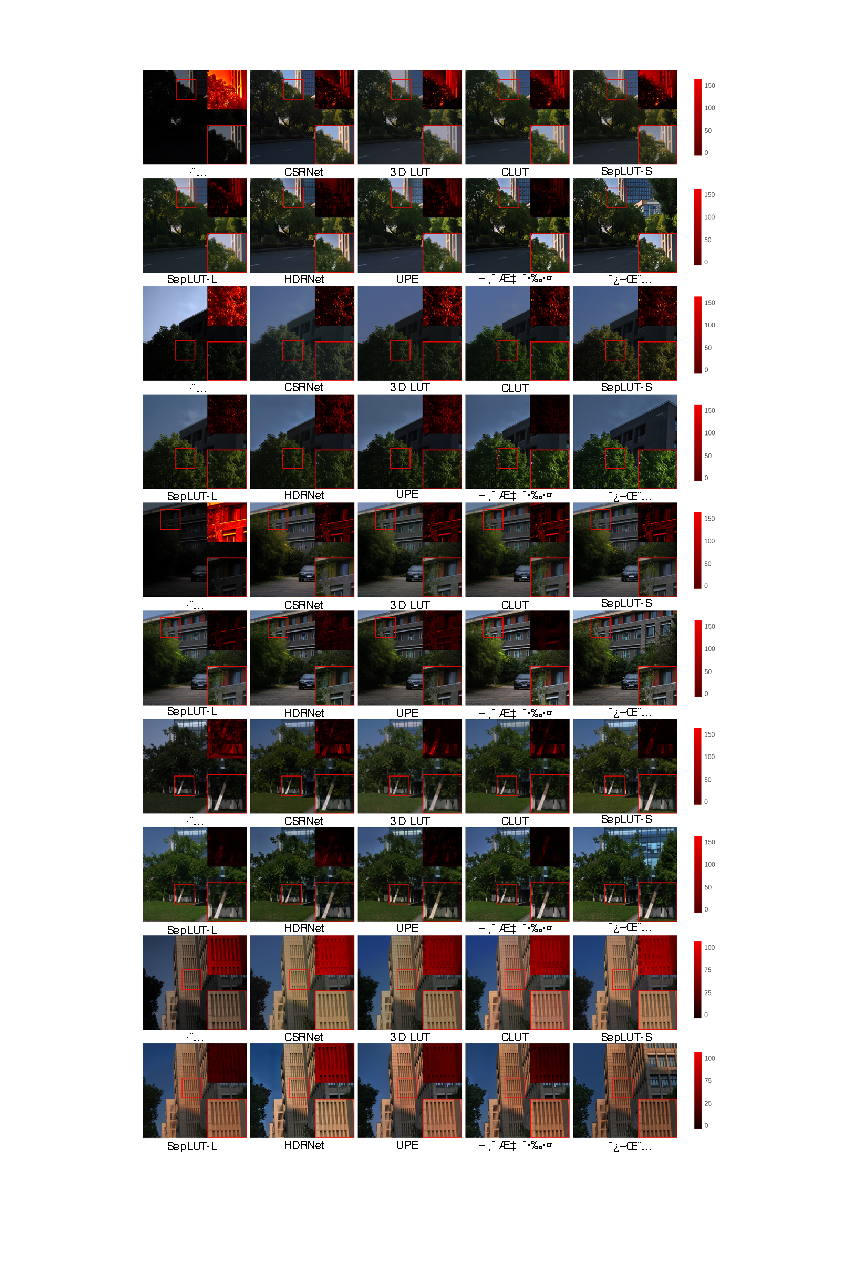
\includegraphics[width=0.9\linewidth]{docs/fig-chap3/fig-3-result-long.pdf}
	\caption{定性比较\quad 每张图片右上角显示的误差图说明了结果与目标图的差异}
	\label{fig:enhance result}
\end{figure*}
图\ref{fig:enhance result}给出了代表性例子的定性比较。本文提出的方法得到的结果在绿植区域表现出增强的对比度和更宽的动态范围,而其他方法增强出的色彩则显得比较暗淡。本文提出的方法得到的结果在墙面区域与目标图的颜色偏差较小,表明光谱信息集成对于提高摄影真实感方面产生了明显的提升。


从以上样本中,可以得出以下结论:(1)在局部亮度剧烈变化的区域,例如具有不同光影分布的阳光下的树叶,本文提出的方法通过去除图像的阴影分量$S$,自适应地进行高动态范围的场景的色调调整。(2)将低空间分辨率光谱图像的反射率分量$R$与扩展的颜色通道相结合,使得用本文提出的方法得到的色调增强结果相比于目标图有最小的颜色偏差。但考虑到Mobile-Spec数据集以天空和绿植为主,蓝色和绿色等冷色调占据了大部分颜色,导致对红色等较暖色调的映射学习不足,今后需要在数据集中扩充暖色调样本。

引入额外的低空间分辨率光谱图像可以在一定程度上缓解不同颜色之间学习的不平衡性。与其他方法相比,本文提出的方法获得了更准确和更符合人眼感受的颜色。

由上述实验结果可以看出,本文提出的方法在阴影和反射率先验的引导下,对于高动态范围的场景,获得了更加准确和令人愉悦的颜色。

定性比较强调了将图像分解为阴影、反射率的有效性。该框架为色调增强提供了明确的引导,并克服了光谱图像的内在复杂性。通过对低空间分辨率光谱图像在色调增强任务中的探索,可以为光谱信息在移动摄影中的应用奠定基础。

\subsection{定量分析}
\begin{table}[h]
\caption{不同图像增强算法的定量比较}  %表标题
\label{tab:j4} 
\begin{tabular}{c|cccccccc}
\hline
 & {CSRNet} & {3D\; LUT} & {CLUT} & {SepLUT-S} & {SepLUT-L} & {HDRNet} & UPE   &本方法            \\ \hline
PSNR↑                               & 26.34                      & 27.52                      & 27.30                    & 27.57                        & 28.08                        & 27.75                      & 28.19 & \textbf{29.83} \\
SSIM↑                                 & 0.923                      & 0.926                      & 0.938                    & 0.933                        & 0.944                        & 0.939                      & 0.946 & \textbf{0.967} \\
$\Delta E^*$↓                                   & 6.44                       & 5.39                       & 4.63                     & 5.37                         & 4.26                         & 5.12                       & 4.79  & \textbf{3.60} \\ \hline
\end{tabular}
\end{table}
% 与其他方法相比,深度照片增强器(Deep Photo Enhancer, DPE)\cite{J6}由于其不成对的设置,导致输出图像受到生成对抗网络引入的非期望伪影的影响,表现出较差的性能。
将本文提出的方法与现有的基于颜色变换的方法进行了图像增强任务的对比分析。在表\ref{tab:j4}中,基于MLP的方法,条件序列修饰网络(Conditional Sequential Retouching Network, CSRNet)\cite{J14}的PSNR略低,为26.34dB。相比之下,基于LUT的方法,如3D\; LUT\cite{J38}、CLUT\cite{J40}、SepLUT-S\cite{J35}等,PSNR相近,在27.30-27.57dB之间。值得注意的是,具有较大参数的SepLUT-L表现出了优越的性能,PSNR达到了28.08dB,这是由于SepLUT-L同时利用1D和3D\; LUT进行增强,其中1D\; LUT以图像自适应的方式调整图像对比度,实现了更均匀的对比度分布。此外,UPE\cite{J33}利用平滑损失约束,估计了一个图像到光源的映射,该映射专为增强不同光源条件下的图像而设计,并取得了良好的处理性能,PSNR达到了28.19dB。

由表\ref{tab:j4}可知,本文方法的图像增强性能达到了目前领先的水平,先前已有的方法在学习HDR场景下准确的色调映射方面面临挑战,而本文提出的方法通过有效地利用阴影和反射率先验来提供明确的引导,PSNR达到了29.83dB,比先前最优的方法提高了5.8\%。

% \subsection{消融实验}
为了避免分解不准确的影响,本实验将阴影先验和反射率先验(记为$S^*$, $R^*$)的理想值单独整合到HDRNet基线中进行验证。

\textbf{阴影先验$S^*$}

\begin{table}[h]
\centering                % 表格居中
\caption{阴影先验的影响}  %表标题
\label{tab:j1a} 

\begin{tabular}{cccc|cccc}
\hline
       & PSNR↑ & SSIM↑ & $\Delta E^*$↓ &           & PSNR↑ & SSIM↑ & $\Delta E^*$↓  \\ \hline
HDRNet & 27.75 & 0.939 & 5.12 & HDRNet+$S*$ & 28.68 & 0.957 & 4.29 \\ \hline

\end{tabular}
\end{table}
从表\ref{tab:j1a}可以看出,HDRNet基线的PSNR为27.75dB,而引入阴影先验$S^*$后使得本文提出的方法得出的PSNR提高到28.68dB。值得注意的是,在这个实验中,HDRNet的结构保持不变,只是将输入的RGB图像转换到反射率空间,就得到了上述的明显提升。

这一发现表明,使用阴影先验$S^*$将原始图像转换到反射率图像是一种简单而有效的色调增强任务设计,在不同的高动态范围场景中表现出普遍的适应性。

\textbf{反射率先验$R^*$}

鉴于光谱成像能力在移动设备上的实际限制,本文开展了消融研究,以考察低空间分辨率光谱图像的光谱和空间分辨率配置对图像增强的影响。首先将空间分辨率保持在默认设置16\times16,并提取不同光谱范围的波段。低空间分辨率光谱图像有10个波段,波长范围为400-1000nm,每个波段带宽为60nm。值得注意的是,400-760nm包含6个可见光波段,而760-1000nm包含4个近红外波段。
\begin{table}[h]
\centering                % 表格居中
\caption{反射率先验在不同波段的影响}  %表标题
\label{tab:j1b} 
\begin{tabular}{c|ccc}
\hline
波段范围            & PSNR↑ & SSIM↑ & $\Delta E^*$↓ \\ \hline
% baseline    & 28.68 & 0.957 & 4.29 \\ \hline
400-520 nm  & 28.74 & 0.957 & 4.00 \\
520-640 nm  & 29.09 & 0.964 & 3.82 \\
640-760 nm  & 29.19 & 0.962 & 3.92 \\
400-760 nm  & 29.24 & 0.967 & 3.72 \\
760-1000 nm & 29.07 & 0.965 & 3.88 \\
400-1000 nm & 29.68 & 0.968 & 3.55 \\ \hline
\end{tabular}
\end{table}
如表\ref{tab:j1b}所示,使用越靠近红色通道的波长作为图像增强的引导,得到的PSNR越高。可能的解释是,本文构建的数据集的组成中占较大面积的类别是天空和绿植,而红色物体的面积和数量相对有限。因此,在训练过程中,HDRNet基线倾向于优先考虑蓝色和绿色波长而不是红色波长,其中,使用全部10个通道(400-1000nm)组合的效果最好,PSNR达到了29.68dB。

在本文看来,细粒度的光谱信息增强了双边网格的颜色感知能力,并补偿了不同颜色通道的不平衡学习。

\begin{table}[h]
\centering                % 表格居中
\caption{不同空间分辨率的反射率先验的影响}  %表标题
\label{tab:j1c} 
\begin{tabular}{c|ccc}
\hline
空间分辨率                      & PSNR↑                     & SSIM↑                     & $\Delta E^*$↓                     \\ \hline
% 基准                    & 28.68                     & 0.957                     & 4.29                     \\ \hline
1\times1                         & 29.05                     & 0.963                     & 4.06                     \\
4\times4                         & 29.21                     & 0.963                     & 3.80                     \\
16\times16                       & 29.68                     & 0.968                     & 3.55                     \\
64\times64                       & 29.81                     & 0.969                     & 3.47                     \\ 
256\times256 & 29.78 & 0.967 & 3.49   \\  \hline
\end{tabular}
\end{table}

在下一个实验中,使用全部10个通道,空间分辨率从1\times1逐步调整到256\times256。如表\ref{tab:j1c}所示,随着空间分辨率的提高,各项评价指标有提高的趋势。考虑到光谱图像在移动设备上空间分辨率的限制,本文认为低空间分辨率光谱图像的最优参数配置可能与双边网格的空间分辨率(16\times16)对齐,也就是低分辨率图像流输入的空间分辨率(256\times256)对应的16倍下采样。

实验结果表明,光谱图像16\times16的空间分辨率配置在引导RGB图像增强时产生了令人满意的结果,在更高的空间分辨率上的实验结果有明显的边际效应。

\section{本章小结}
先前的方法在学习高动态范围场景下准确的色调增强方面面临挑战,而本文提出的方法通过有效地利用阴影和反射率先验来提供明确的引导。通过大量的实验和测试,证明了本文提出的方法在动态范围压缩和色调映射上相对于已有的方法有所提升。这主要归功于本章方法在以下几个方面的研究:

1.利用室外太阳光近红外波段近似出的阴影图,提出了局部亮度适应法,调节高动态范围RGB图像不同区域的亮度。

2.通过将光源光谱作为图像增强网络的额外输入,提出了光谱感知自注意机制,将光源光谱嵌入到RGB特征图中,提升了RGB图像色调映射的效果。

本章虽然在图像的动态范围压缩和色调映射上进行了研究,在图像锐度增强、去噪、除雾等方面还缺少研究,值得在未来进一步研究光源光谱对这些方面的辅助效果。本方法使用推扫式高光谱相机获取的图像引导RGB的图像增强,在商用高端智能手机上目前还无法实现高精度的光谱图像采集,需要进一步探索受限的光谱成像对RGB图像增强的帮助。

% 本研究中低空间分辨率光谱图像的空间分辨率固定为16\times16,这在商用高端智能手机上目前还无法实现。
% 提高空间分辨率将提高联合分解模型中阴影和物质先验的预测精度。在移动设备上的图像增强和相关应用的背景下,需要进一步探索解决受限的光谱成像能力。
%---------------------------------------------------------------------
%	第四章
%---------------------------------------------------------------------
\chapter{光源光谱校正的材质分割}
\section{引言}
材质分割是一个重要的研究课题,从视觉外观中识别材料对计算机视觉任务至关重要,特别是那些涉及与现实世界交互的任务。

在高光谱图像研究中,分割和分类之间的边界并不清楚。图像分类通常是指给整个图像分配一个或多个标签的任务,而图像分割是指为图像中的每个像素分配一个类别。大量关于高光谱图像分类的研究实际上都是在进行语义分割。例如,高光谱图像分类\cite{S18,S19,S2}中最先进的方法通过分割模型来进行逐像素的分类。

高光谱图像分类问题是根据每个像素向量的光谱或光谱空间特性为其分配一个类别标签的任务,这与计算机视觉中的语义分割任务密切相关,相应地,高光谱图像的材质分类任务也与材质分割任务高度相关。对于与材质相关的高光谱图像中的每个像素,都对应一个由反射率数据组成的向量。这些向量形成了一个宽度为$w$、高度为$h$和波段数为$c$的高光谱数据立方体$(w\times h\times c)$。在RGB图像中$c = 3$,而在高光谱图像中$c$可以高达数百。由于不同的材质有它们本征的光谱反射率特征,可以利用这些信息将高光谱图像的像素进行分类。

鉴于高光谱图像具有更精细的光谱细节特征以及图谱合一等优势,其被广泛应用于分类、检测和分割等任务。Ahmad等人\cite{ahmad2021hyperspectral}回顾了从传统方法到深度学习模型的高光谱图像分类,Su等人\cite{su2021hyperspectral}回顾了高光谱目标定位中的异常检测方法,Huang等人\cite{huang2021weakly}探索了在城市道路场景的高光谱图像的语义分割,Liang等人\cite{liang2022multimodal}在RGB、偏振和近红外图像中实现了多模态的材质分割。尽管现有的基于高光谱图像的分类、检测和分割方法已经取得了显着的成效,但是其中大多数方法都忽略了场景光源条件的影响。

在本章中,本文使用光源光谱校正的方式,得到不同材质的本征光谱反射率特征,从而将高光谱图像更有效地运用于材质分割。为支撑本文的深度学习算法,本文提出了RGB图像与高光谱图像对齐的材质分割数据集。考虑到跨模态数据总量的平衡,本文使用高空间分辨率的RGB图像和低空间分辨率且具有多通道的光谱图像相结合的方式进行材质分割,从而将高光谱图像光谱特征更细的优势带给RGB图像,提高材质分割的准确度。



\section{相关研究 }
\subsection{基于阴影和反射率先验的本征分解}
光谱反射率与物体材质直接相关,使用基于阴影和反射率先验的本征分解能将与光源和形状无关的反射率提取出来。

一种研究思路是用物体的形状及其造成的阴影作为约束条件。Barron和Malik\cite{IID1,IID2,IID3}提出了三个假设:(1)物体形状的曲率变化较小,表面较为光滑;(2)表面法线的取向是各向同性的,物体表面可以朝向任何一个方向;(3)在被遮挡物体的边界附近,表面法线的方向朝向外部;根据这三个假设进行图像本征分解。Chen等人\cite{IID7}对RGB-深度(RGB-D)图像进行本征分解,通过RGB图像和深度图像消除预测的阴影的歧义。Jeon等人\cite{IID13}假定光源平滑变化且物体表面为朗伯表面,据此确定物体表面法线,作为本征分解的约束条件。

另一种研究思路是从反射率本身出发进行本征分解。Shen等人\cite{IID26}利用物体表面色调的局部连续性作为约束,求解物体的反射率。Zhou等人\cite{IID32}提出了一种数据驱动的图像本征分解方法,通过在人工标注的反射率数据集上训练一个模型来预测反射率。Zoran等人\cite{IID33}提出了从灰度图像中分辨光照变化的方法。Shen和Yeo\cite{IID27}利用纹理的局部连续性将原始图像分离为阴影和反射率。

在本章中,本文利用第三章提出的数据集中阴影图作为训练样本,将本征分解和材质分割两个问题同时求解。

\subsection{基于Transformer的语义分割}
材质分割作为与语义分割相接近的研究问题,因为目前相应的数据集匮乏,一种做法是通过特殊的设计来实现特定材质的区分,而另一种做法是将语义分割的方法迁移到材质分割任务中。

近年来,学者将基于Transformer的方法应用于语义分割,取得了显著的成效。Zheng等人\cite{T5}将语义分割作为一个序列到序列的预测任务,采用一个纯Transformer作为其分割模型的编码器,而不使用任何卷积层,增大了模型的感受野,从全局提取信息,提高了语义分割整体的准确度。Liu等人\cite{T4}通过层次特征映射将Transformer中计算自注意的复杂度从平方复杂度降低到线性复杂度,并将滑动窗口法改进为移位窗口法,大幅度降低延迟。Strudel等人\cite{T11}提出的方法包含一个在ImageNet上预训练的ViT\cite{T2}(Vision Transformer)主干网络,并引入一个掩码Transformer作为解码器,使用预训练好的模型在中等大小的图像分割数据集上进行微调,提高了训练效率。Wang等人\cite{T71,T72}通过引入一个渐进收缩的金字塔主干网络来降低计算成本,同时输出粒度更细的分割结果,从而克服了ViT的问题。Ranftl等人\cite{T74}提出了一种基于Transformer的编码器-解码器结构的密集预测模型,能够在Transformer架构的所有阶段中保持空间分辨率,为密集预测任务保留了细粒度信息。

与成熟的卷积神经网络不同,Transformer仍处于发展的早期阶段,且需要比CNN更多的训练数据,因此对于材质分割,尤其是高光谱图像的材质分割这种缺少数据集的任务来说,Transformer的潜力还未完全发挥出来。

为此,本章利用Transformer在语义分割中的最新研究,结合第二章相关研究中介绍的用于高光谱图像的Transformer中光谱自注意的提取方法,将RGB图像与高光谱图像相结合,并使用第二章中得到的光源光谱进行反射率校正,有效提高材质分割的精度。
%不具备跨数据集的泛化性。%从分割任务的通用性出发,我们将介绍几个基于Transformer的语义分割方法。

% \textbf{\textbf{SE}gmentation \textbf{TR}ansformer (SETR)}

% SETR\cite{T5}将语义分割作为一个序列到序列的预测任务,采用一个纯Transformer作为其分割模型的编码器,而不使用任何卷积层。
% \begin{figure*}[h]
% 	\centering
% 	%\fbox{\rule{0pt}{2in} \rule{0.9\linewidth}{0pt}}
% 	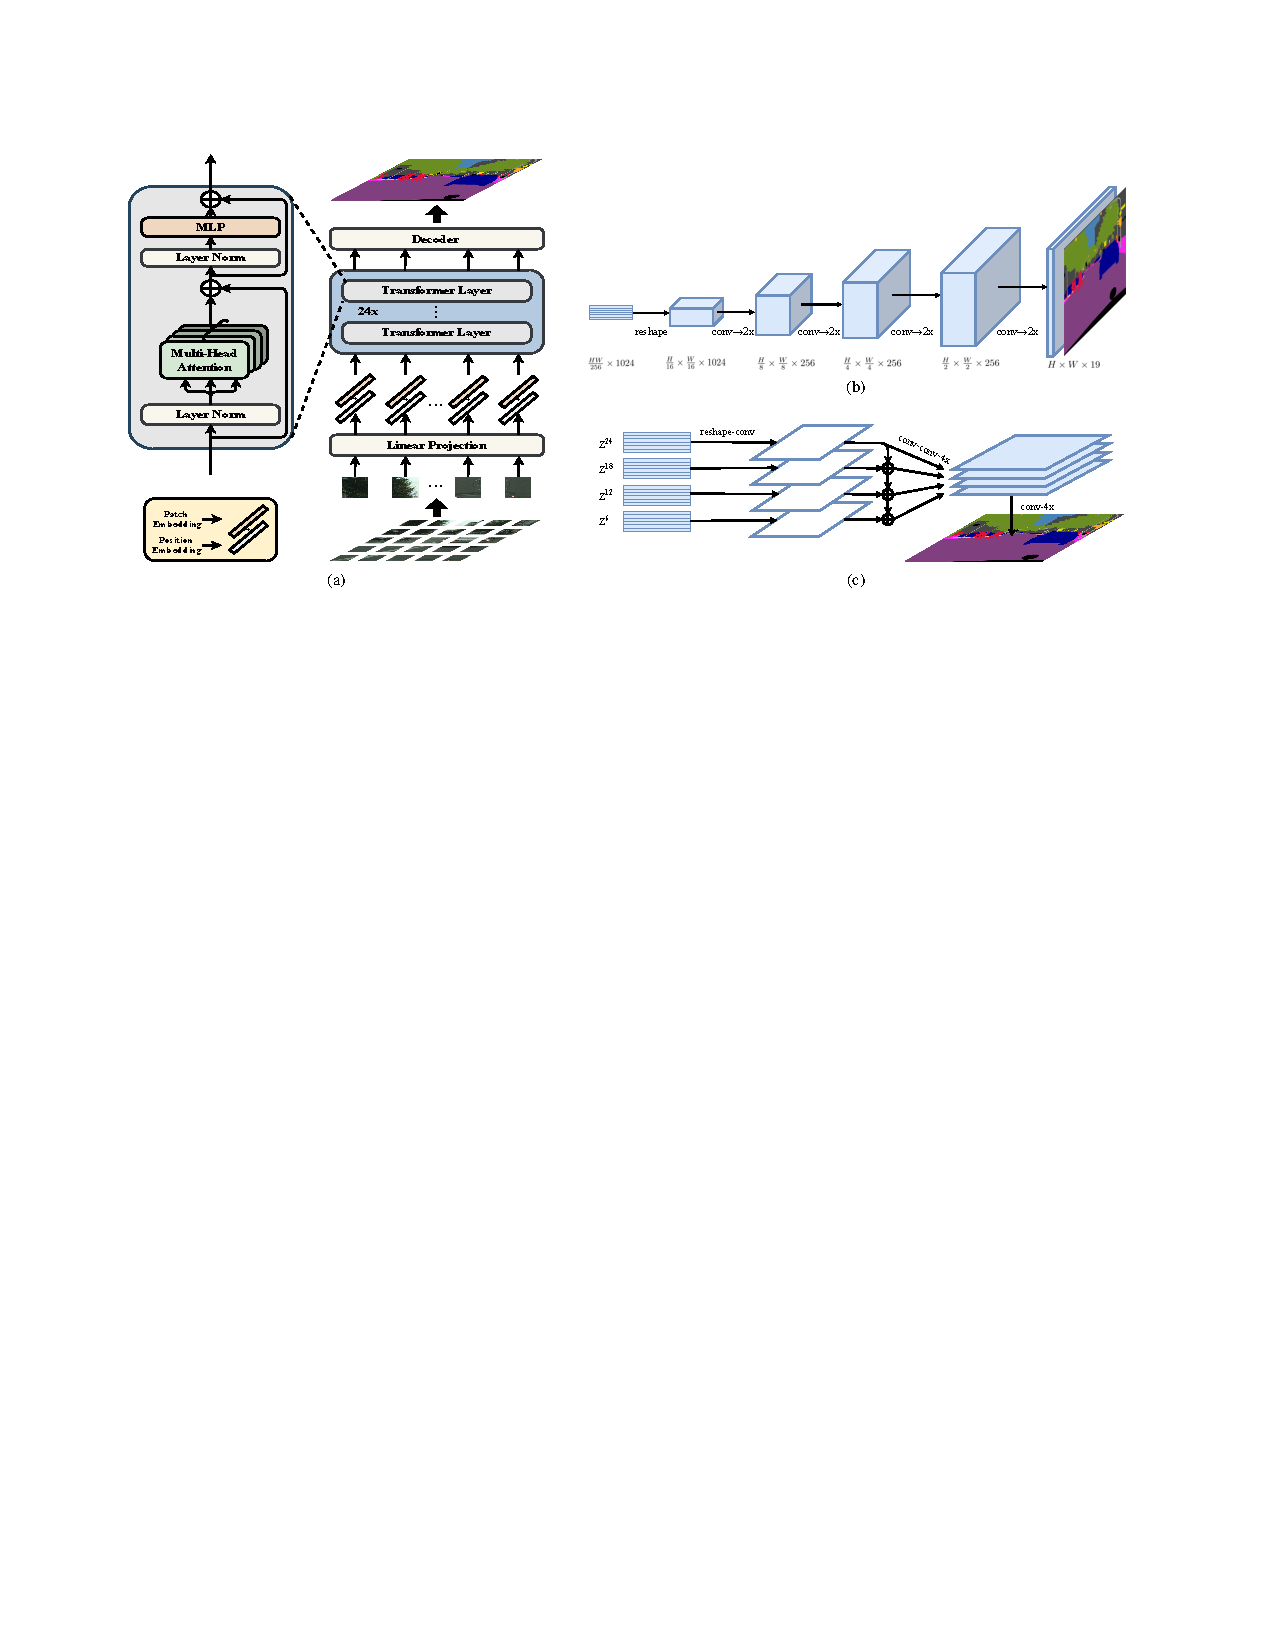
\includegraphics[width=1.0\linewidth]{docs/fig-chap4/fig-4-setr.pdf}
% 	\caption{SETR的结构示意图\cite{T5}\quad (a) SETR由一个标准的Transformer组成\quad (b) SETR-PUP的渐进式上采样设计\quad (c) SETR-MLA的多层次特征聚合结构}
% 	\label{fig:setr}
% \end{figure*}

% 如图\ref{fig:setr}(a),SETR编码器有着标准的Transformer处理流程,将一个图像视为一系列的图像块,然后进行线性投影,使用图像块编码和位置编码将这些投影嵌入到一组Transformer层中。SETR在每层编码器Transformer的空间分辨率上没有下采样,而是只提供全局的上下文建模。SETR还有几种变体,图\ref{fig:setr}(b)展示了渐进式上采样(Progressive UP-sampling, PUP)的SETR的结构,图\ref{fig:setr}(c)展示了多层次特征聚合(Multi-Level feature Aggregation)的SETR的结构。

% \textbf{Swin Transformer}

% Swin Transformer\cite{T4}(Hierarchical Vision Transformer using Shifted Windows)是为了解决计算机视觉任务没有通用Transformer这一问题而提出的,可以作为通用骨干网络用于计算机视觉任务如图像分类和密集的预测。
% \begin{figure*}[h]
% 	\centering
% 	%\fbox{\rule{0pt}{2in} \rule{0.9\linewidth}{0pt}}
% 	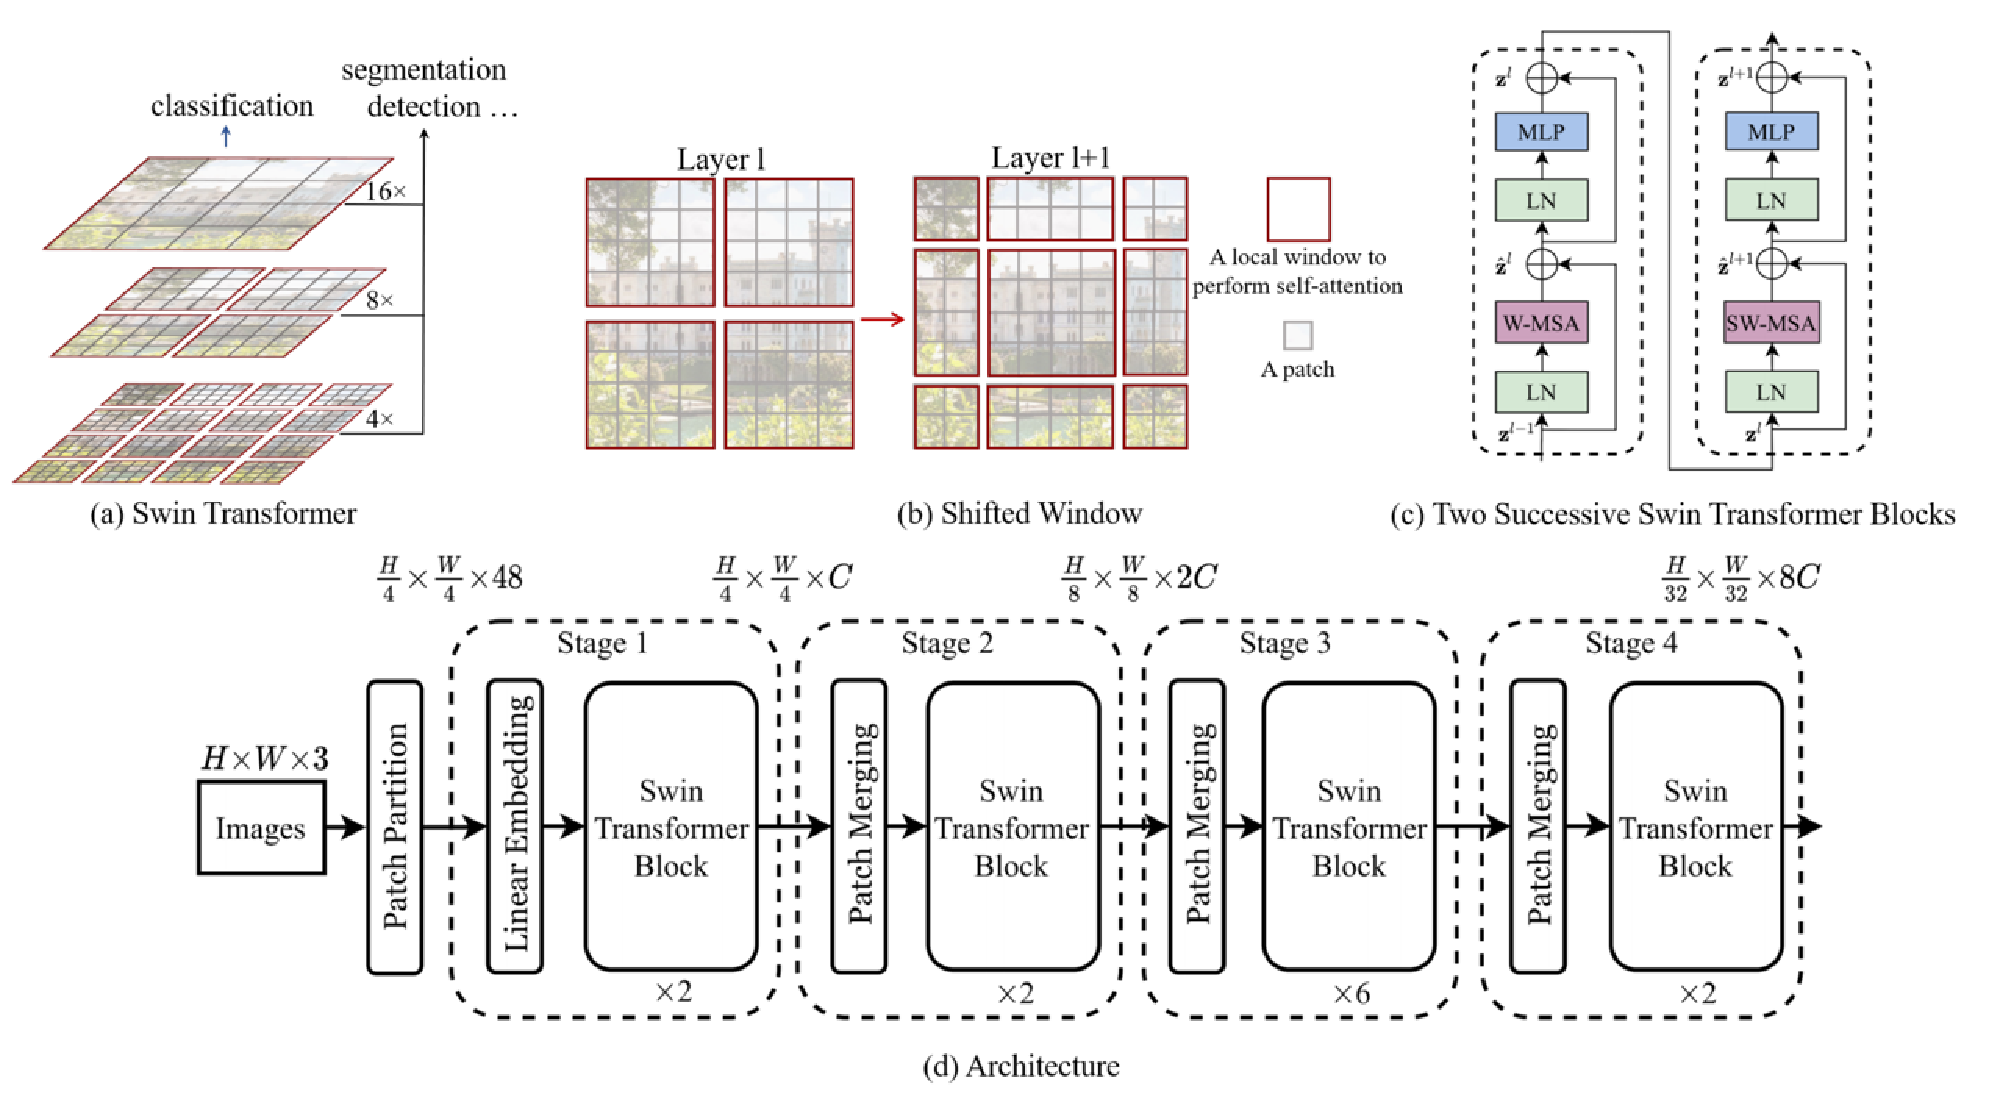
\includegraphics[width=1.0\linewidth]{docs/fig-chap4/fig-4-swin.pdf}
% 	\caption{Swin Transformer的结构示意图\cite{T4}\quad (a)层次特征映射,用于降低计算复杂度\quad (b)移位窗口法\quad (c)模块间的串联\quad (d)Swin的核心架构}
% 	\label{fig:swin}
% \end{figure*}
% Swin变换器通过构造层次特征映射,将Transformer中计算自注意的二次计算复杂度降低到线性复杂度。此外,图\ref{fig:swin}中所示的移位窗口方法比早期用于计算自注意的基于滑动窗口的方法的延迟要低得多。

% 根据Swin Transformer的架构,在一开始,它使用patch分区模块将给定的图像分割成一系列不重叠的图像块。然后对该图像块序列应用线性嵌入,将其投射到任意维度中。接下来是几个双Transformer块应用自注意。图像块合并模块的主要职责是减少更深层次中的token数量。值得注意的是,层次阶段的特征图分辨率与典型的对15润滑结构,如ResNet\cite{T68}相似。因此,Swin Transformer可以在计算机视觉任务中有效地取代ResNet主干网络。

% \textbf{Segmenter}

% Segmenter
% Strudel等人\cite{T11}提出的方法包含一个在ImageNet上预训练的ViT\cite{T2}(Vision Transformer)主干网络,并引入一个掩码Transformer作为解码器,使用预训练好的模型在中等大小的图像分割数据集上进行微调,提高了训练效率。
% \begin{figure*}[h]
% 	\centering
% 	%\fbox{\rule{0pt}{2in} \rule{0.9\linewidth}{0pt}}
% 	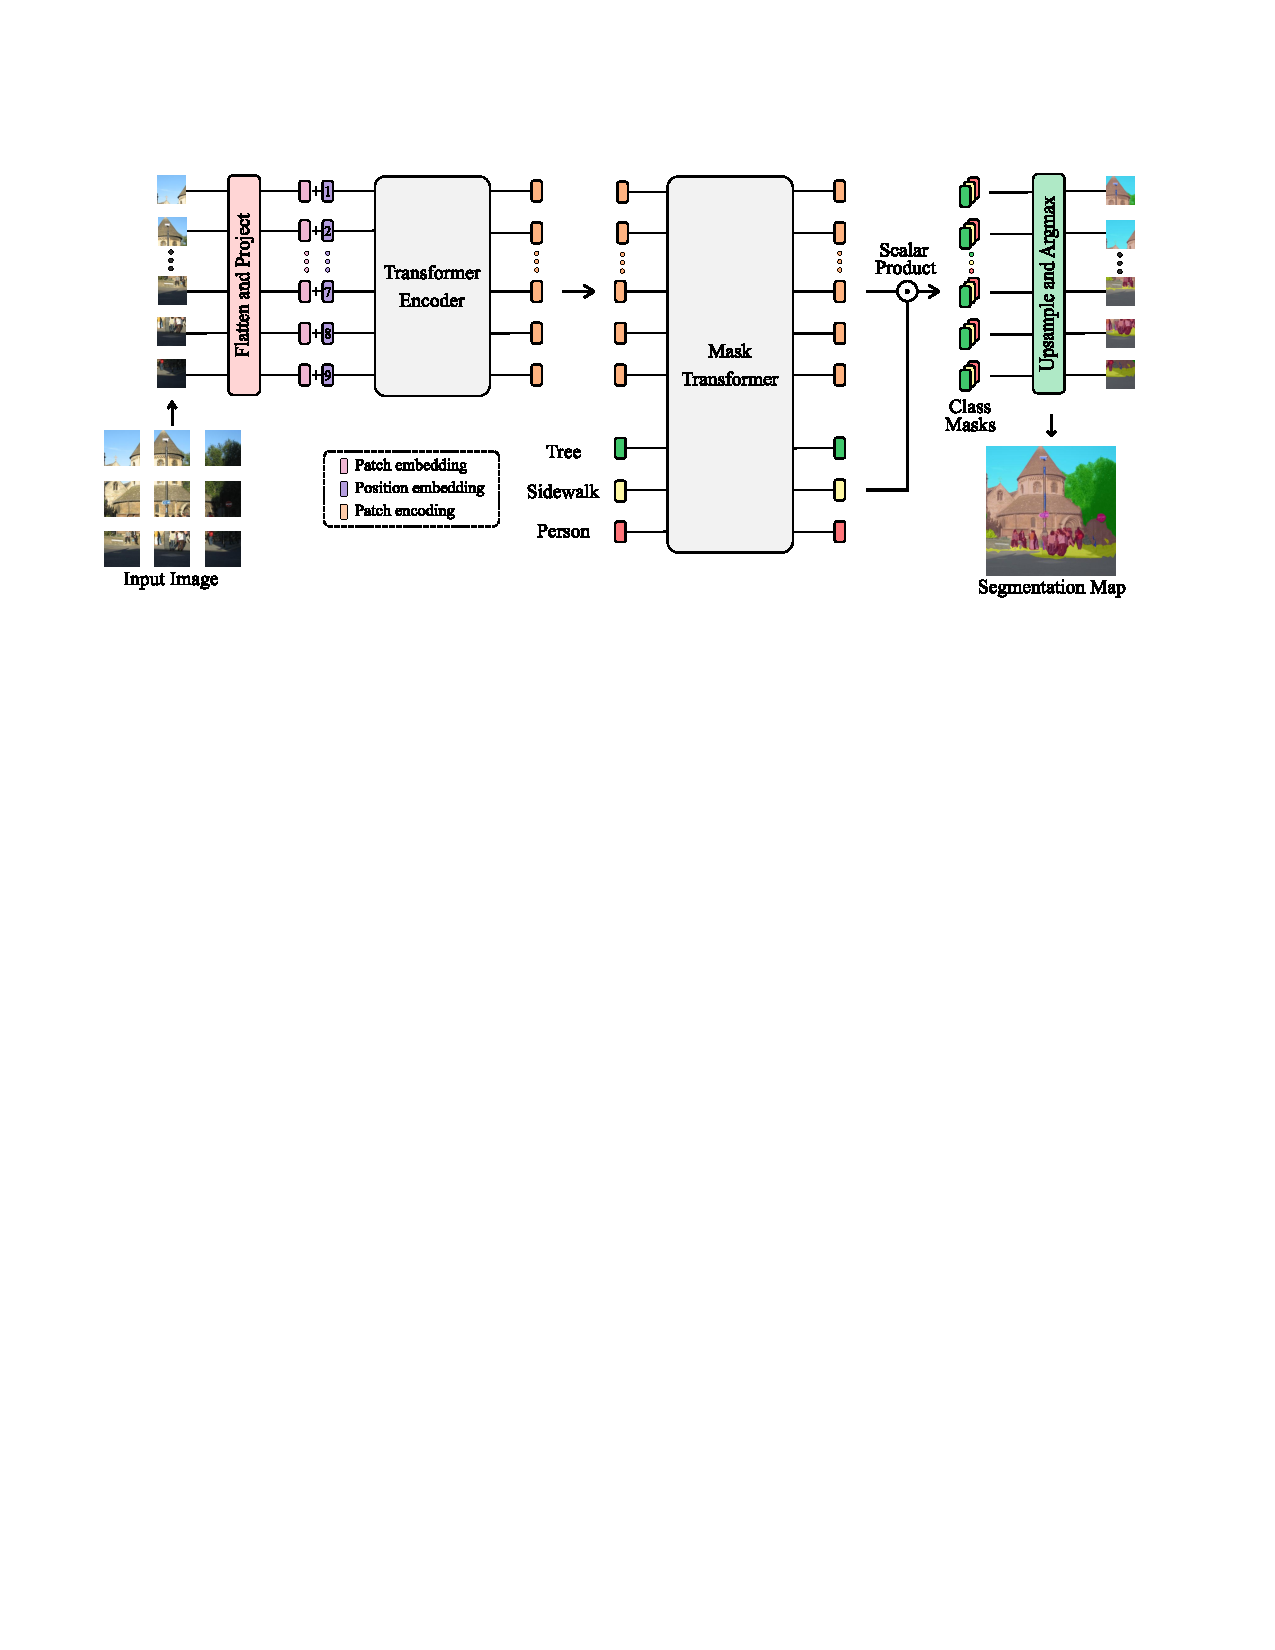
\includegraphics[width=1.0\linewidth]{docs/fig-chap4/fig-4-segmenter.pdf}
% 	\caption{Segmenter的结构示意图\cite{T11}\quad 基本上有一个ViT主干和一个掩码Transformer作为解码器}
% 	\label{fig:segmenter}
% \end{figure*}

% 基于CNN的模型在处理全局图像上下文时通常效率较低,最终导致次优的分割结果,原因在于卷积是一种局部操作,难以获取图像的全局信息。全局交互的建模需要对图像的每个原始像素之间的交互进行建模,因此具有平方复杂度。Segmenter的体系结构特别善于捕捉图像的全局上下文。除了语义分割任务,Segmenter模型还可以通过改变模型体系结构来应用于全景分割(语义分割+实例分割)任务。在这种情况下,模型的类嵌入(class embeddings)需要被替换为对象嵌入(object embeddings)。

% \textbf{Pyramid Vision Transformer (PVT)}

% PVT

% 是纯Transformer的、用于密集预测的通用骨干网络,如图\ref{fig:pvt}所示。ViT输出的特征图是单一尺度的,而且分辨率通常较低,计算成本也比较高,所以ViT一般不能直接适用于密集的预测任务。PVT\cite{T71,T72}通过引入一个渐进收缩的金字塔主干网络来降低计算成本,同时输出更细粒度的分割结果,从而克服了ViT的问题。
% \begin{figure*}[h]
% 	\centering
% 	%\fbox{\rule{0pt}{2in} \rule{0.9\linewidth}{0pt}}
% 	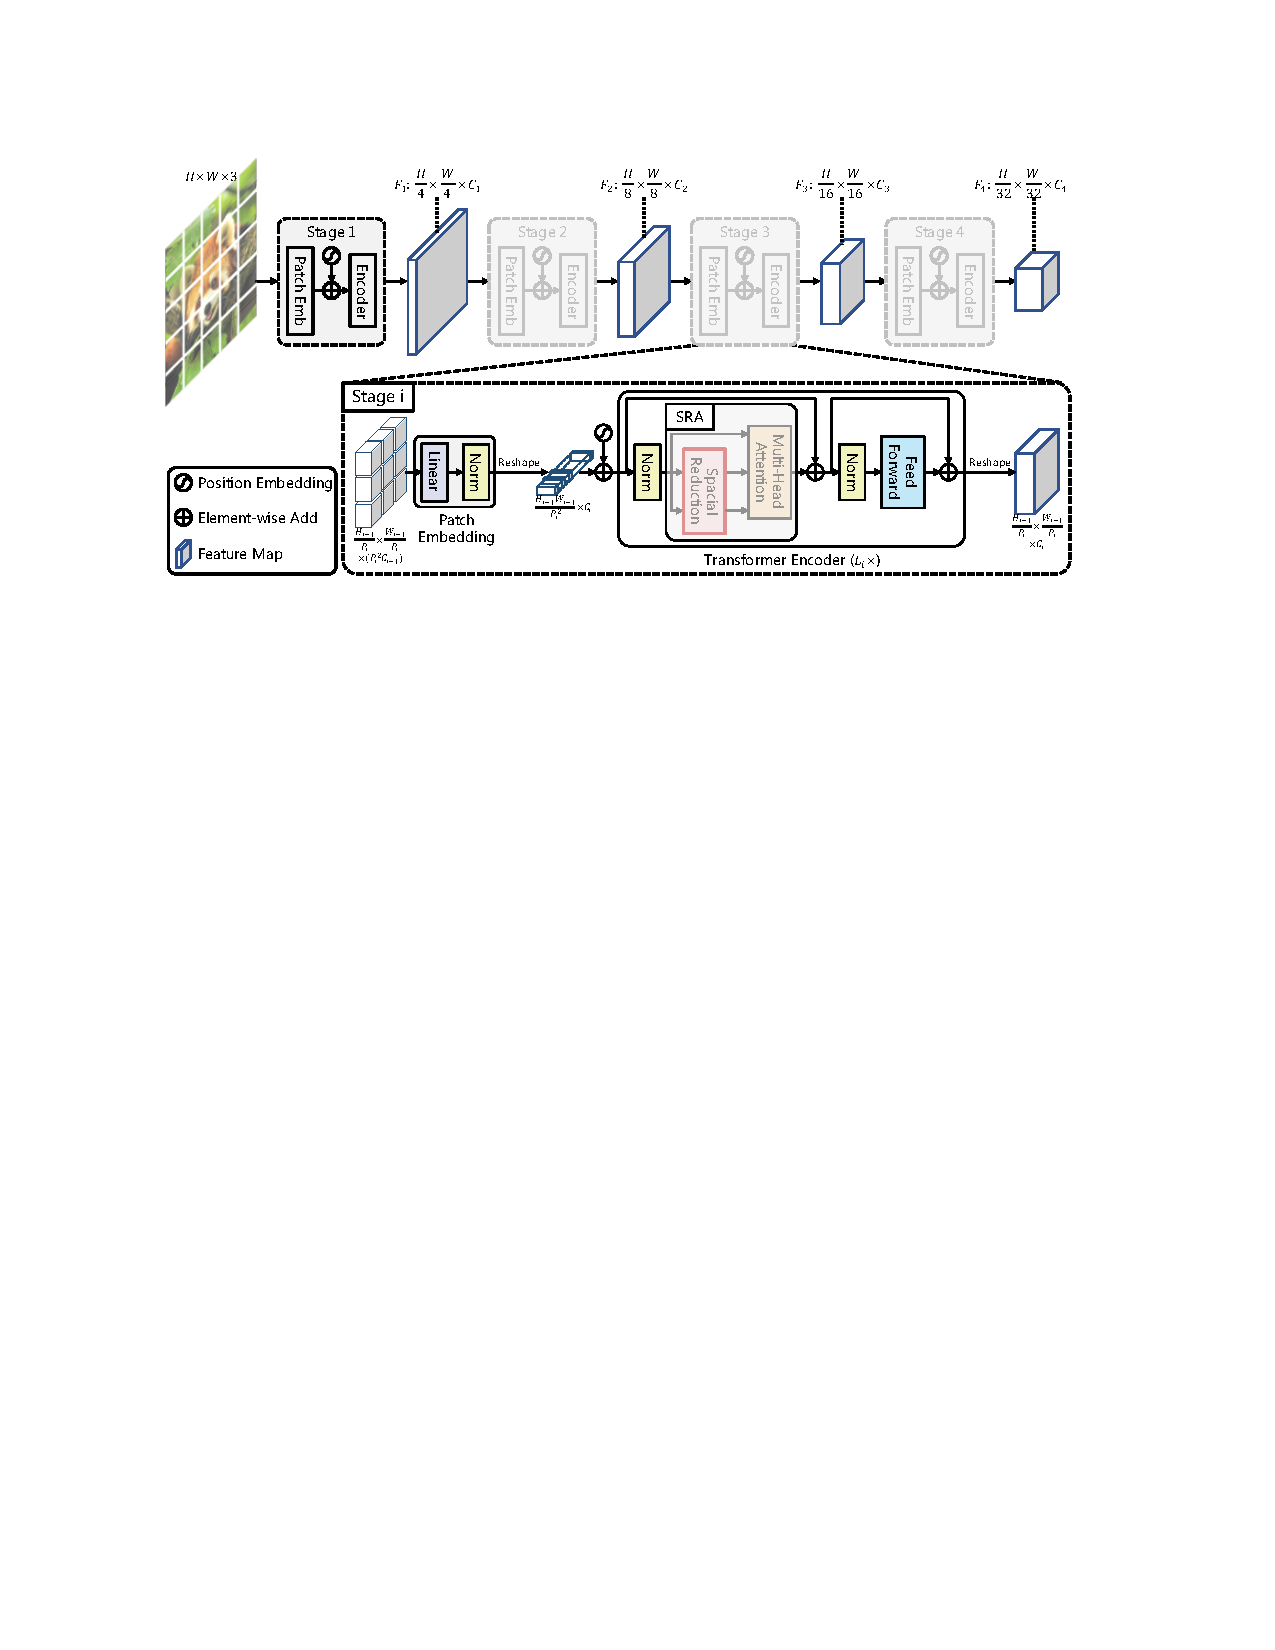
\includegraphics[width=1.0\linewidth]{docs/fig-chap4/fig-4-pvt.pdf}
% 	\caption{PVT的结构示意图\cite{T71}\quad 各阶段的金字塔结构逐渐缩小了特征图的分辨率}
% 	\label{fig:pvt}
% \end{figure*}
% 与ViT相比,PVT\enspace v1版本有一些显著的区别。与ViT使用16\times16个图像块相比,PVT\enspace v1使用4\times4个图像块作为输入,因而提高了模型学习高分辨率表示的能力,通过使用一个渐进收缩的金字塔,减少了传统ViT的计算需求,这种金字塔结构在负责生成可缩放的特征图的阶段中,逐步将输出分辨率从高到低缩小。PVT\enspace v1用一种新的空间缩减注意层(Spatial
% Reduction Attention, SRA)取代了ViT中的多头注意层(Multi-Head Attention, MHA),从而使得注意操作前的空间尺度缩小,进一步降低了算力的需求。

% PVT\enspace v1版本也有一些缺点,例如,在处理高分辨率图像时,PVT\enspace v1的计算量需求相对较大。又如,将图像作为一系列不重叠的图像块进行处理时,会失去图像的局部连续性。再如,由于位置编码的大小是固定的,PVT\enspace v1不能处理大小变化的输入。

% PVT\enspace v2版本有三个主要的改进,规避了以前的设计缺陷。首先是线性空间缩减注意(Linear
% Spatial Reduction Attention, LSRA),它使用平均池化将图像的空间分辨率降低到一个固定的大小,与PVT\enspace v1中的SRA不同,使得LSRA具有线性复杂度。第二,重叠的图像块嵌入,是通过图像边界的零填充和与相邻窗口重叠区域的放大来实现的,有助于捕获更多的图像局部连续性。第三,卷积前馈网络,有助于处理不同分辨率的输入。通过这些改进,PVT\enspace v2能够将PVT\enspace v1的非线性复杂度降低到线性复杂度。

% \textbf{Dense Prediction Transformer (DPT)}

% DPT

% \begin{figure*}[h]
% 	\centering
% 	%\fbox{\rule{0pt}{2in} \rule{0.9\linewidth}{0pt}}
% 	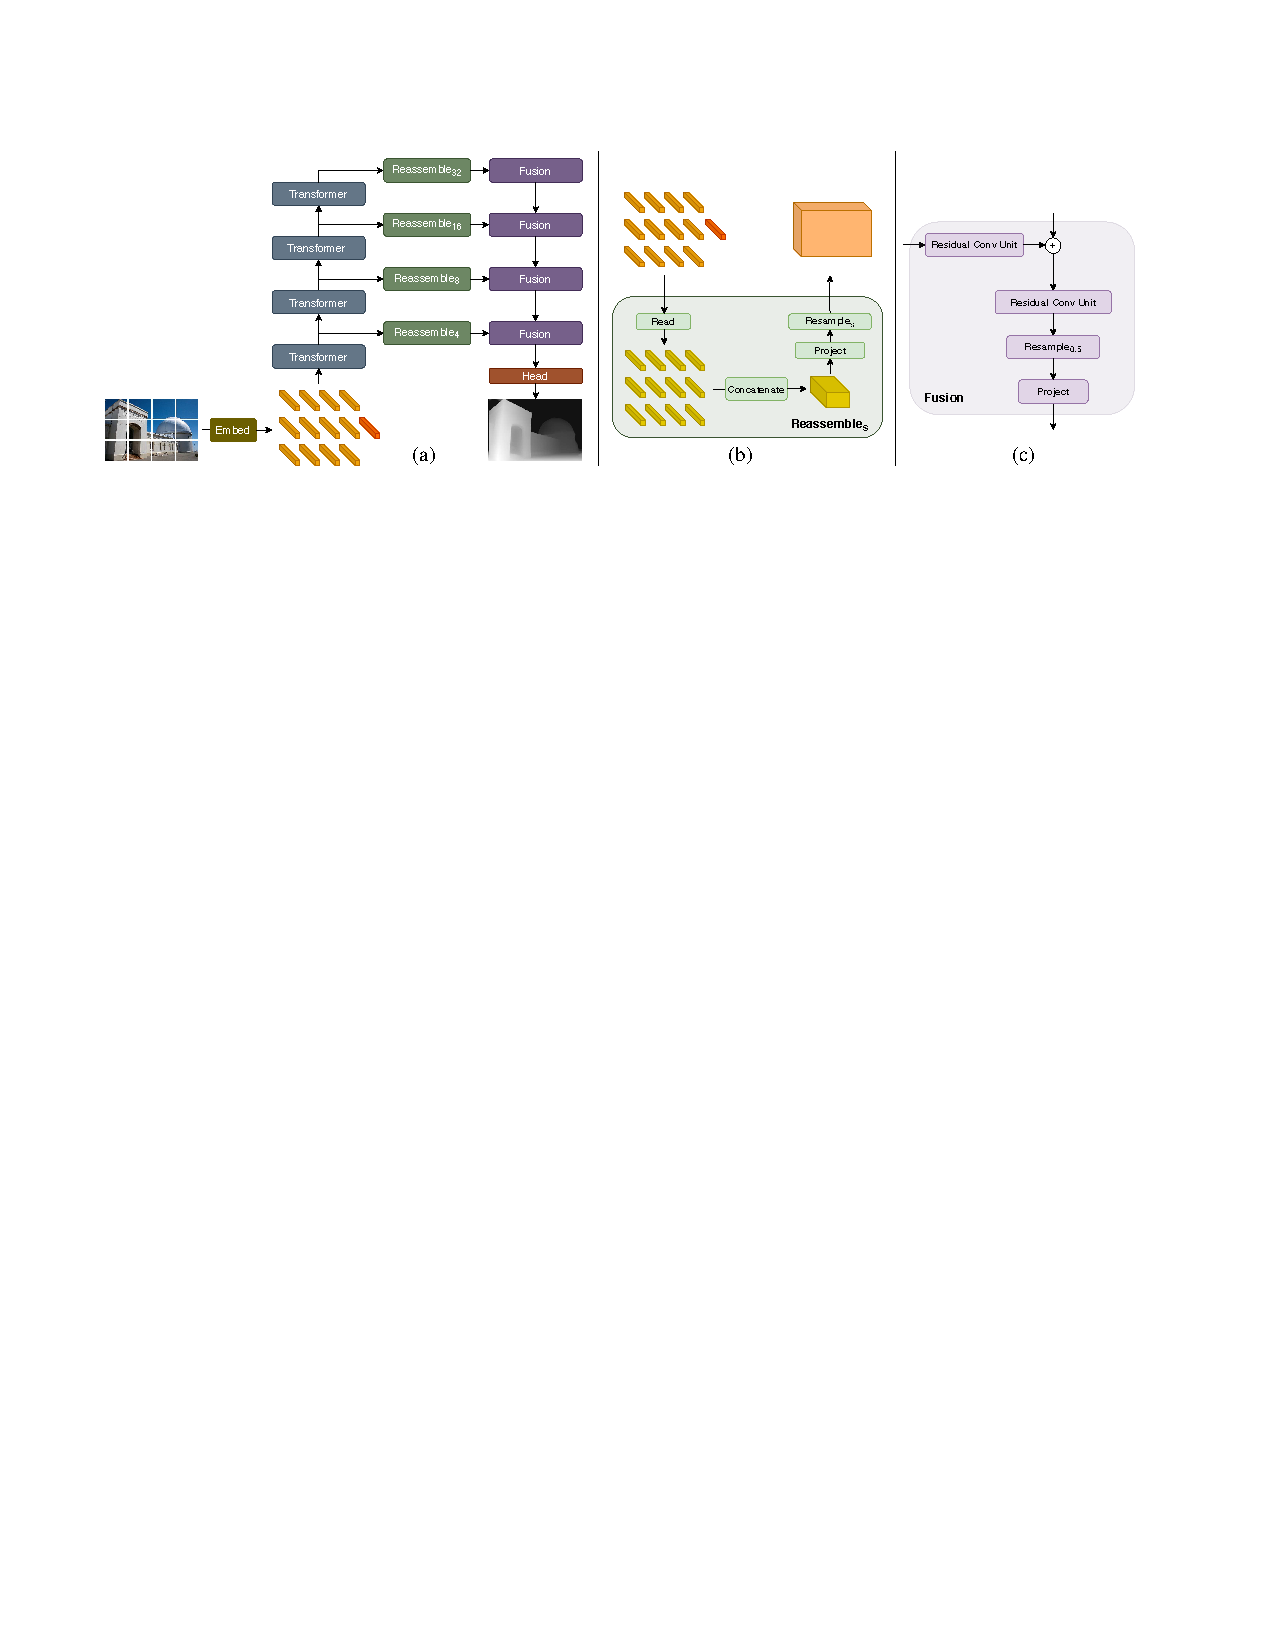
\includegraphics[width=1.0\linewidth]{docs/fig-chap4/fig-4-dpt.pdf}
% 	\caption{DPT的结构示意图\cite{T74}\quad (a)不重叠的图像图像块被输入到Transformer块中\quad (b)将token重新组装到特征图的操作\quad (c) 用于组合特征映射的融合模块}
% 	\label{fig:dpt}
% \end{figure*}

% DPT-Base和DPT-Large模型使用图像块的嵌入,将输入图像分割成非重叠的图像块,然后将这些信息输入到具有可学习位置嵌入的Transformer块中,定位每个独立token的空间位置。DPT-Base有12个Transformer层,DPT-Large有24个Transformer层,后者具有较大的特征尺度。

% 另一种模型是DPT-Hybrid,使用卷积主干网络ResNet-50作为特征提取器,并使用基于像素的特征映射作为12层Transformer块的token输入。如图\ref{fig:dpt}所示,Transformer模块用多头自注意(Multi-head Self-Attention, MSA)\cite{T1}顺序块重新组装token,用于token之间的全局交互。这些token被重新组装成各种分辨率下的类似图像的特征表示,使用解码器中的残差卷积单元将这些表示进行组合,并融合在一起,以进行最终的密集预测。
\section{本文构建的材质分割数据集}
为了支撑本文提出的材质分割算法,本文对第三章中提到的Mobile-Spec数据集进行了材质分割的标注。Mobile-Spec数据集中的阴影图仍被保留,用于RGB图像的反射率校正。
\begin{figure*}[h]
	\centering
	%\fbox{\rule{0pt}{2in} \rule{0.9\linewidth}{0pt}}
	\includegraphics[width=1.0\linewidth]{docs/fig-chap4/fig-4-dataset.pdf}
	\caption{高光谱材质分割数据集}
	\label{fig:seg dataset}
\end{figure*}

如图\ref{fig:seg dataset}展示了本文构建的数据集中的材质分割图像,其中分割类别被指定为绿植、树干、建筑、道路、天空和其他,这些类别反映了室外场景中最常见的对象。本文的材质分割标注具有极高的细粒度,特别是在绿植区域内单个叶片的细节方面。

值得注意的是,在本数据集的标注中,树冠上的树叶与地面上的草和灌木一起被标注为“绿植”,本文认为绿植的光谱特征比较相近,这样的标注方法是区分于语义分割的。不像语义分割中将树干与树叶标注为“树”这一类,本数据集单独对树干进行标注,用于区分其与绿植不同的光谱响应。对于道路和建筑的区分,有些比较矮的围墙与道路相连,本数据集将可供人行走的区域标注为道路,不可供人行走的区域标注为建筑。

\begin{figure*}[h]
	\centering
	%\fbox{\rule{0pt}{2in} \rule{0.9\linewidth}{0pt}}
	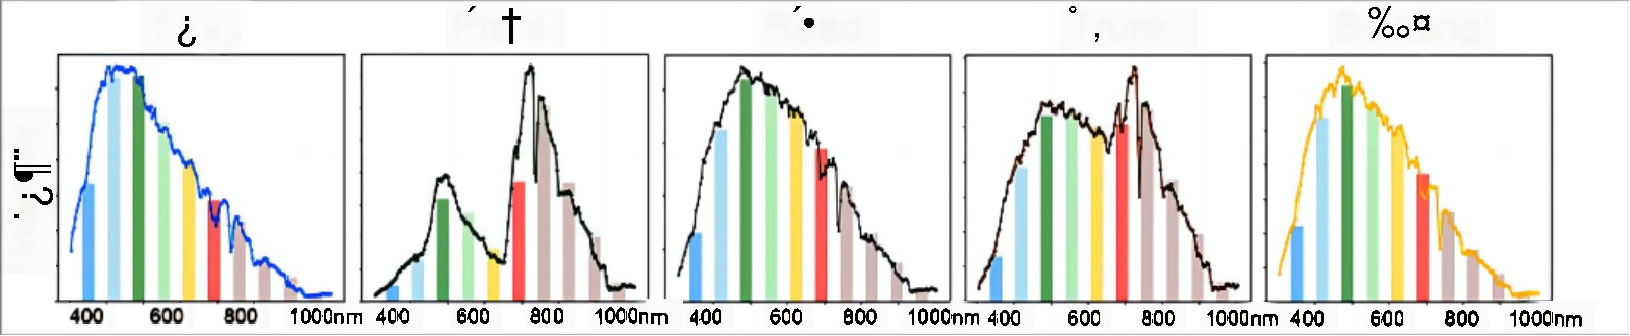
\includegraphics[width=1.0\linewidth]{docs/fig-chap4/fig-4-curve.pdf}
	\caption{不同材质类别的光谱响应曲线}
	\label{fig:seg curve}
\end{figure*}

如图\ref{fig:seg curve}所示,不同的材质类别有着不同的光谱响应,这为材质分割提供了细致的光谱信息依据。其中,蓝色波段(450 - 520 nm)是天空的强反射带;绿色波段(520 - 600 nm)处绿植有一个明显的峰;红色波段(630 - 690 nm)是绿植的主要吸收带;近红外波段(760 - 900 nm)是绿植和树干的强反射带。

\begin{figure*}[h]
	\centering
	%\fbox{\rule{0pt}{2in} \rule{0.9\linewidth}{0pt}}
	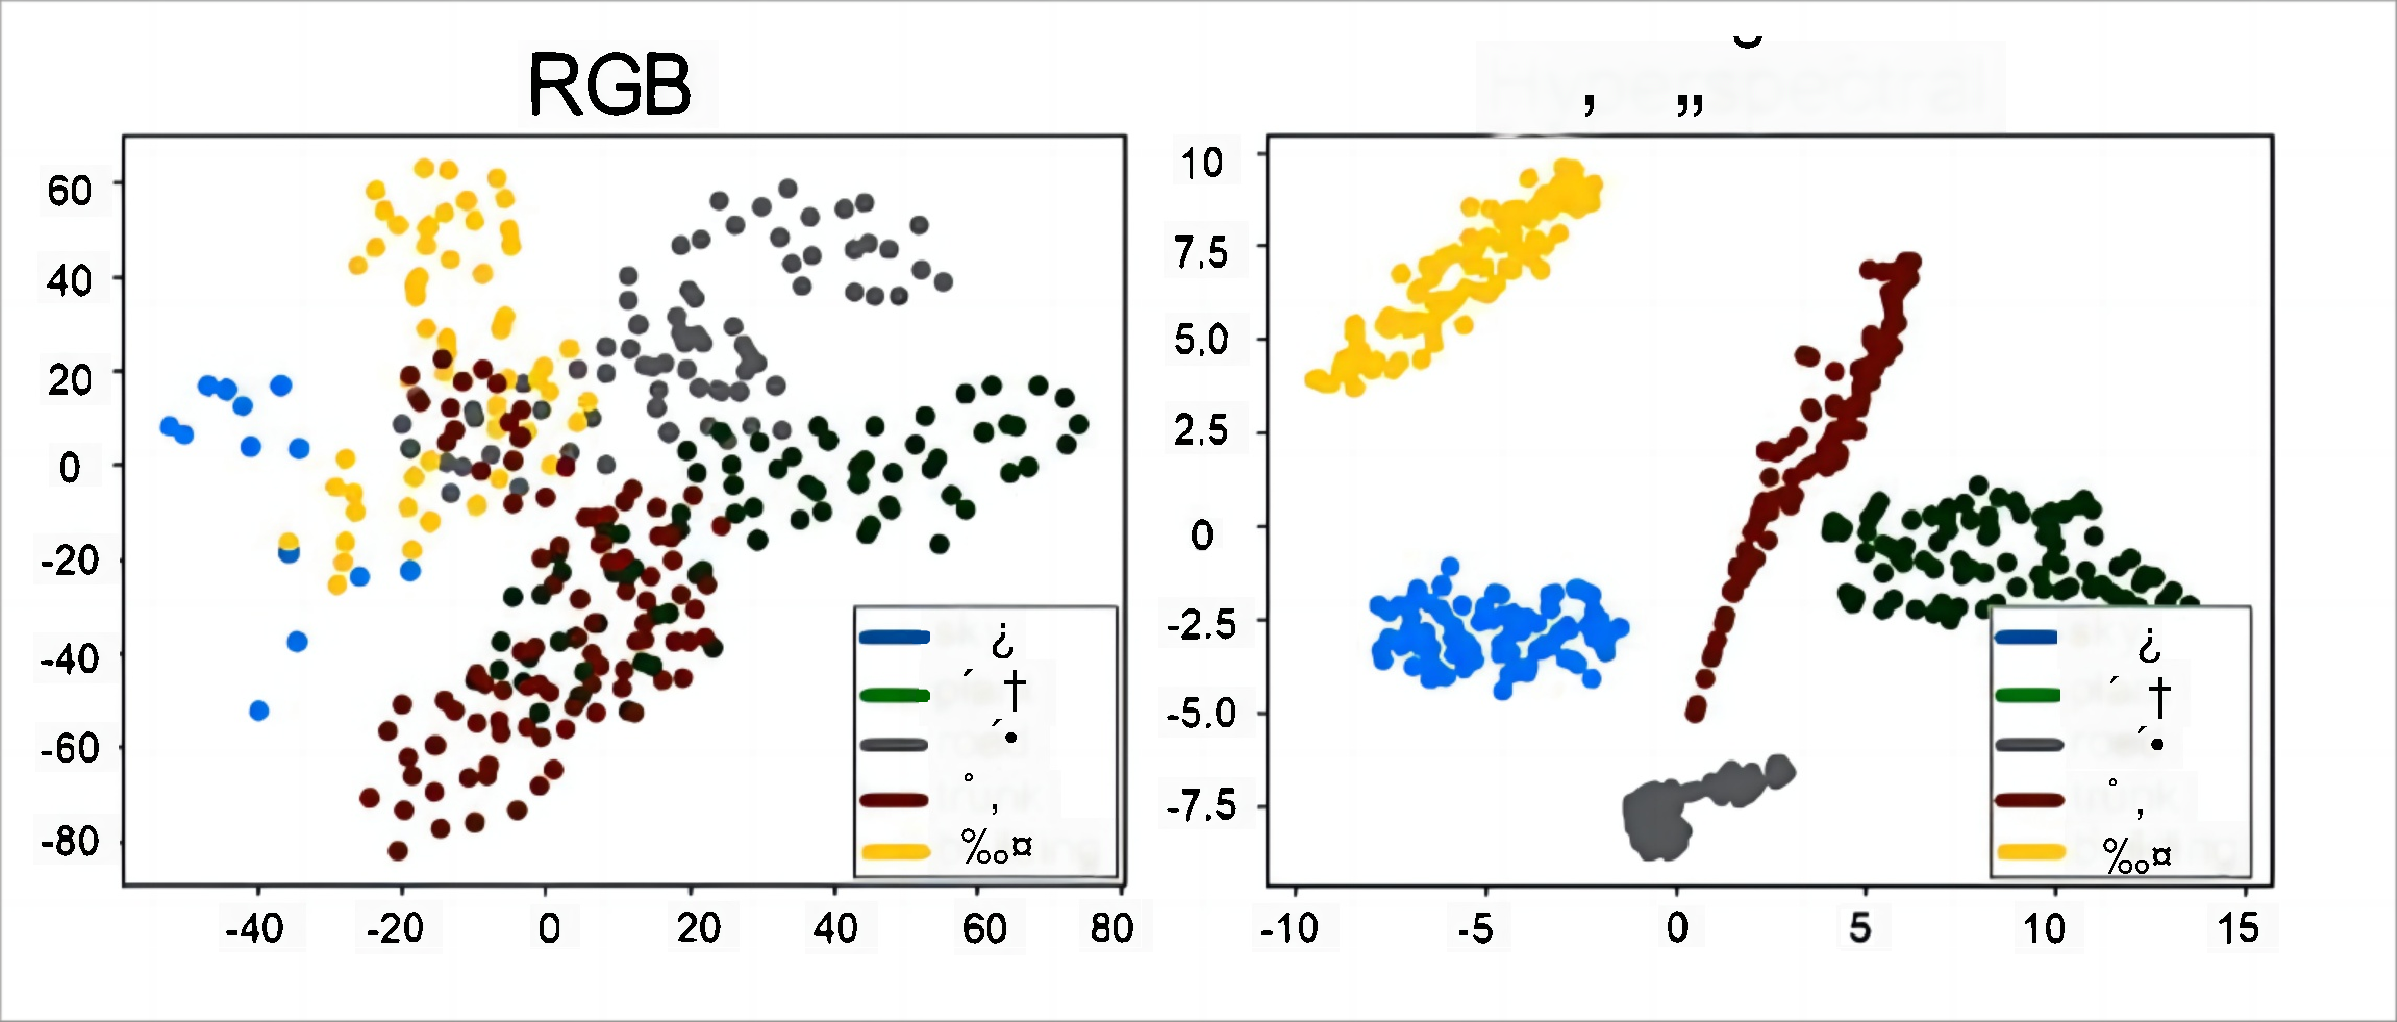
\includegraphics[width=1.0\linewidth]{docs/fig-chap4/fig-4-tsne.pdf}
	\caption{不同材质类别的在RGB域和高光谱域的聚类可视化}
	\label{fig:seg tsne}
\end{figure*}

本文采用t-随机邻域嵌入(t-distributed Stochastic Neighbor Embedding, t-SNE)\cite{J26}来分析复杂的光谱模式和不同光谱波段之间的关系。如图\ref{fig:seg tsne}所示,与RGB图像相比,代表不同类别的特征在高光谱图像的t-SNE可视化中表现出更密集的聚集。这一现象表明,光谱通道数的增加使得对不同材质的辨别变得更加简单,因此,低空间分辨率光谱图像有助于材质分割任务。

% 与RGB图像(1057\times960\times3)相比,低空间分辨率光谱图像具有有限的空间分辨率(16\times16\times10)。考虑到低空间分辨率光谱图像的空间分辨率设置很小,在JDM-HDRNet中对齐误差可以忽略不计。我们相信,高精度的RGB-高光谱图像对对于许多其他任务是有意义的,例如RGB-光谱锐化\cite{A8}、重建\cite{A3}、分割\cite{A5}和光源估计\cite{A10}。因此,我们保证Mobile-Spec数据集保持最小的对齐误差。

% 由于色调映射的目标具有很强的主观性,不同的个体具有不同的审美偏好,因此我们使用商业隐私模型来生成Mobile-Spec数据集的目标,该数据集集成了多个专家的审美。该模型由大规模、高质量的商业数据集训练,并由专业摄影师和艺术家精心调整。然后通过主观评估,综合考虑色差、清晰度、噪声和伪影等因素,对目标图像进行细致的筛选。不符合标准的样本予以剔除。我们采用结构保真项来评价Mobile-Specdataset的客观质量。需要注意的是,由于Mobile-Spec中的色调增强图像是高动态范围场景,不符合一般图像的统计自然性,所以我们只保留了结构保真项,去除了统计自然性项。

\section{本文提出的方法}
在RGB语义分割模型的基础上,本文引入光谱信息作为第二路输入来辅助材质分割。对第二路的光谱信息,首先进行反射率校正的预处理,去除光源和阴影的影响,再使用光谱联合RGB分解模型进一步分解RGB图像的阴影和反射率,将RGB图像的反射率输入材质分割网络,提高材质分割的准确度。

为了将低空间分辨率光谱图像有效地集成到高空间分辨率的RGB图像分割的模型中,本文首先分析了高光谱相机和RGB相机在成像机制上的差异,高光谱相机成像模型\cite{J5,J18}可以表示如下:

\begin{equation}
I_{k, x}=\int_{400 \mathrm{nm}}^{1000 \mathrm{nm}} C_k(\lambda) L(\lambda) S(x) R(\lambda, x) d \lambda, k=1,2,3 \ldots
\end{equation}

$I_{k, x}$表示第$k$波段位置$x$处的像素强度,$C_k(\lambda)$表示相机响应函数,$L(\lambda)$表示光源的光谱曲线,$S(x)$表示阴影,$R(\lambda, x)$表示场景的反射率。对于RGB相机,波段数量仅有3个,且波段范围在可见光范围内。RGB相机与高光谱相机的核心区别在于$C_k(\lambda)$,由于$C_k(\lambda)$具有更高的光谱采样率,高光谱图像具有细粒度的颜色通道。

需要注意的是,本文将光源对光谱数据的影响分解为光源光谱曲线$L(\lambda)$和阴影$S(x)$两项。光源光谱曲线$L(\lambda)$通常由光源估计获得,用于自动白平衡,而阴影$S(x)$和反射率$R(\lambda, x)$两项的作用却很少被研究,本文同时使用光源曲线$L(\lambda)$和阴影$S(x)$来对高光谱和RGB图像进行校正,并将得到的反射率$R(\lambda, x)$用于材质分割。

\subsection{反射率校正预处理}

\begin{figure*}[h]
	\centering
	%\fbox{\rule{0pt}{2in} \rule{0.9\linewidth}{0pt}}
	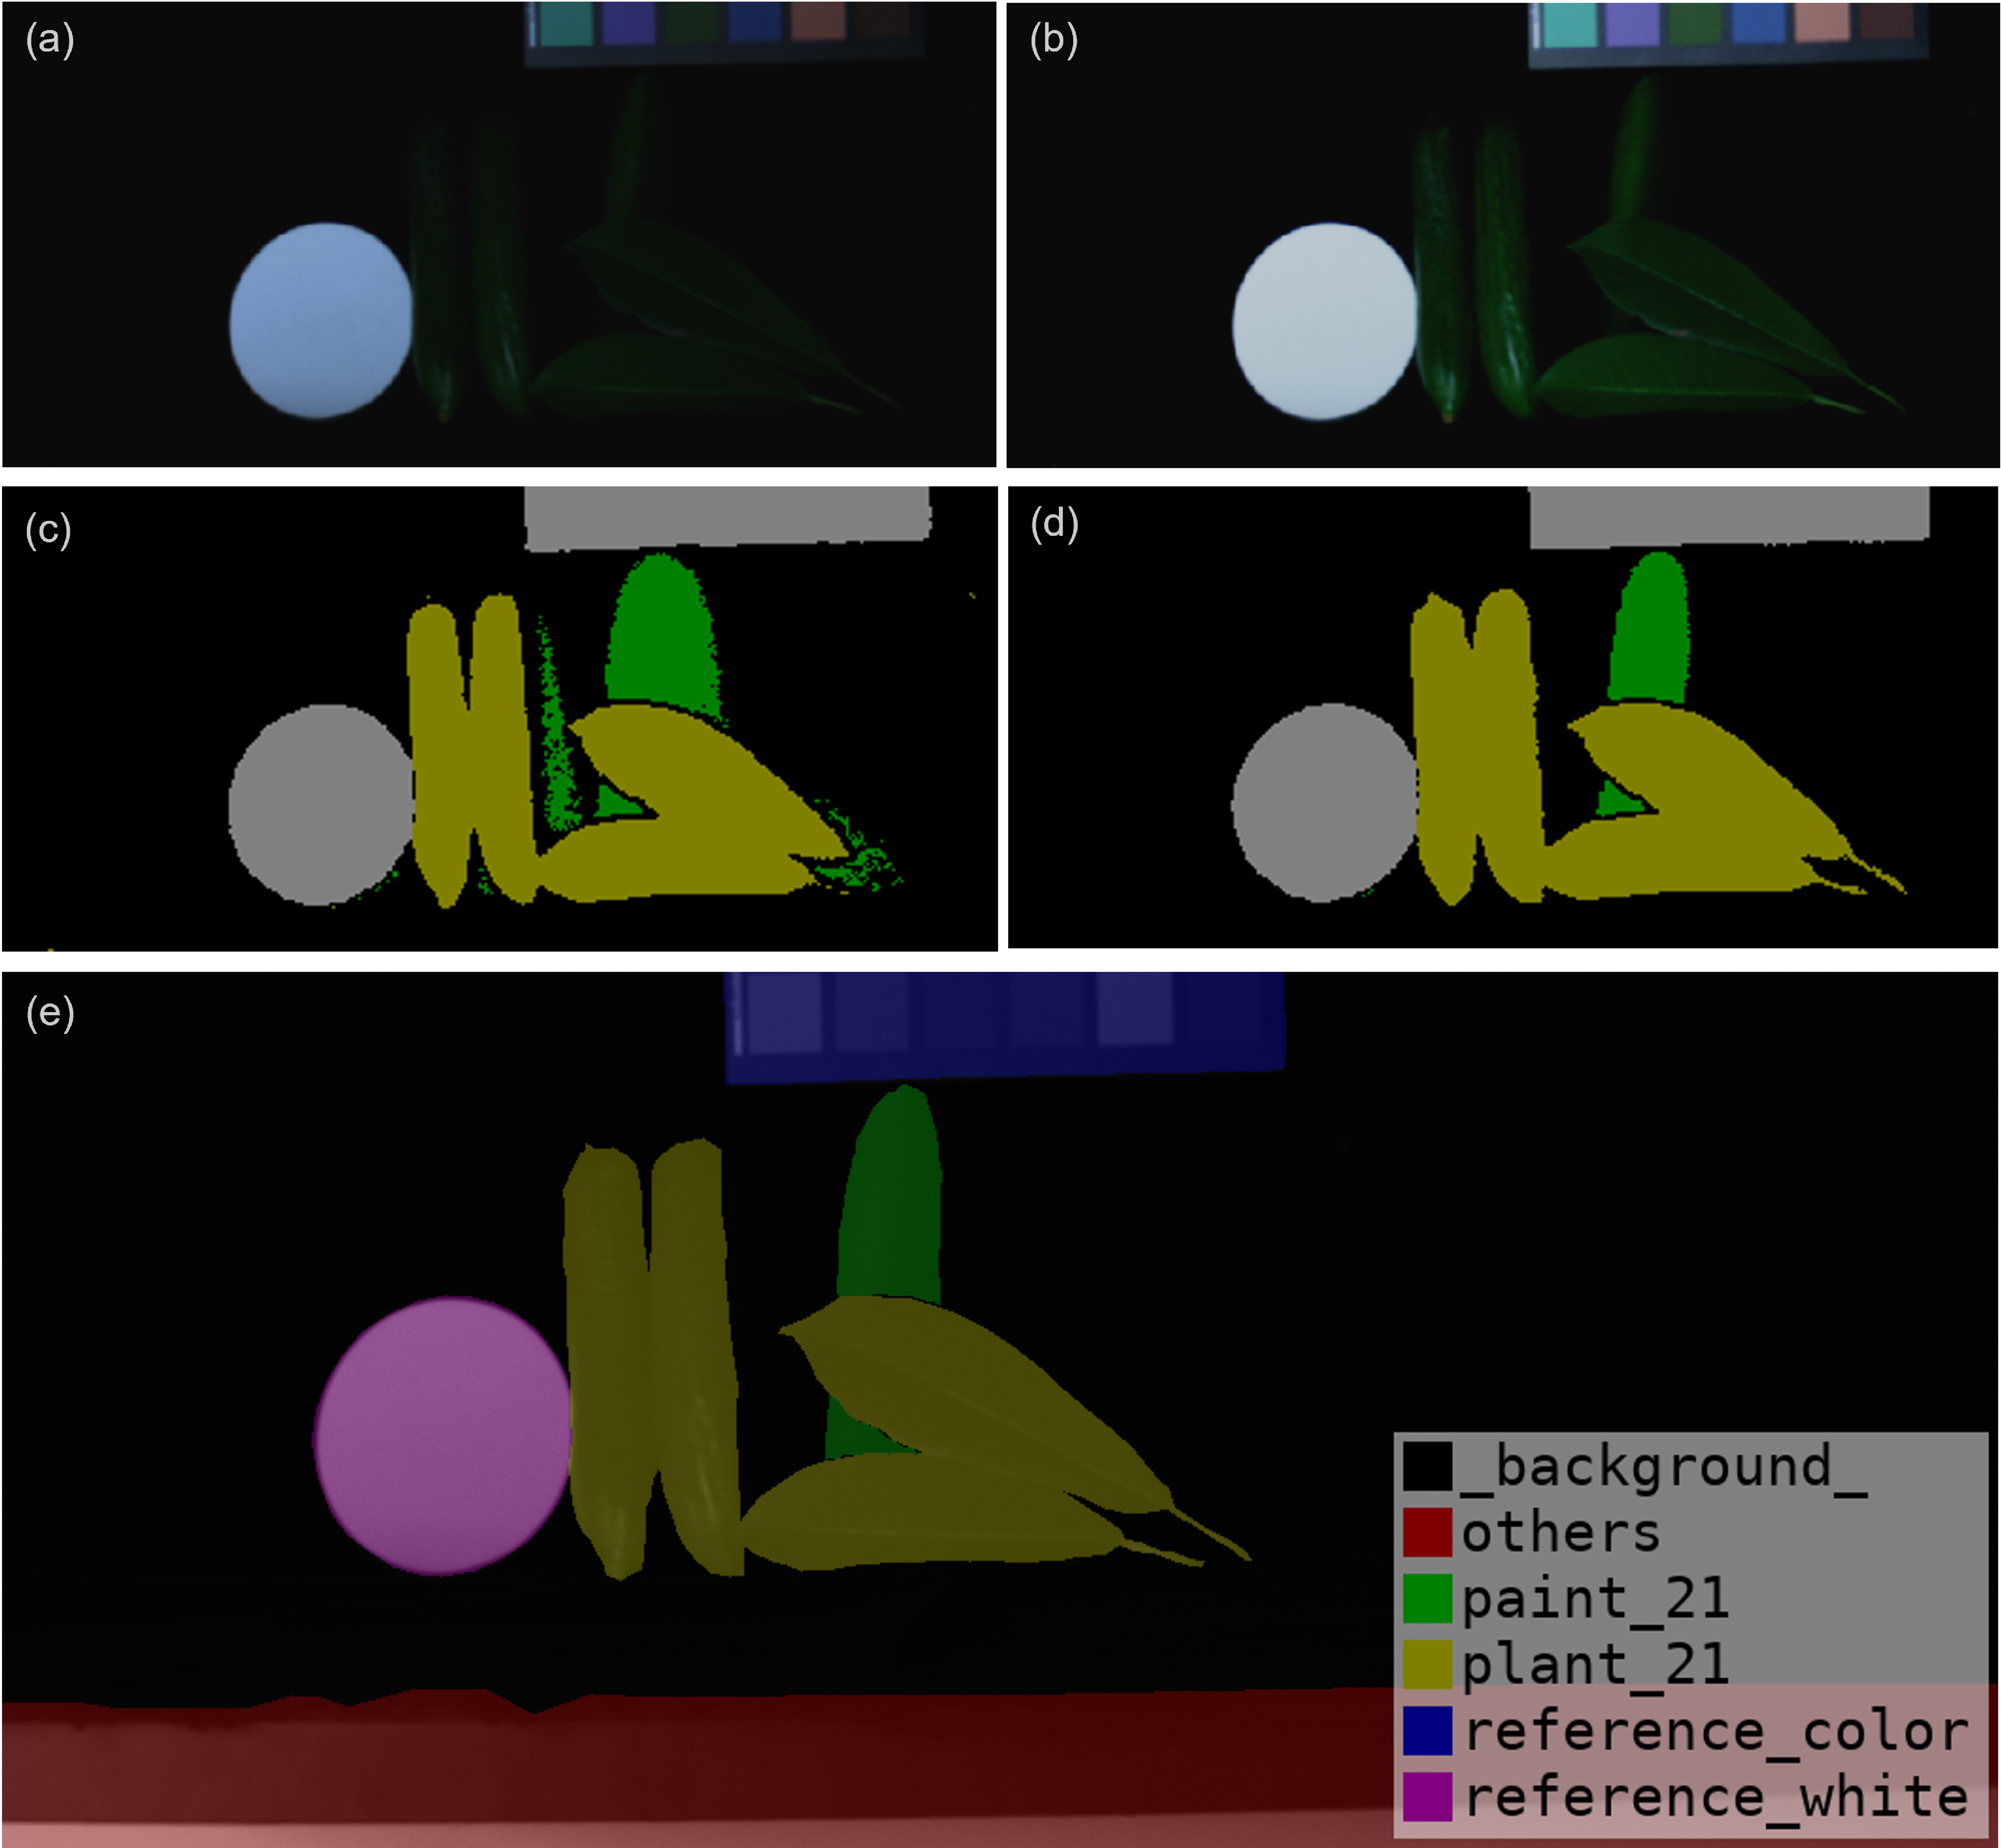
\includegraphics[width=0.8\linewidth]{docs/fig-chap4/fig-4-illu-correct-seg.pdf}
	\caption{对高光谱图像的无监督分割,初步验证光源校正的作用\quad (a)未经校正的图像\quad (b)校正后的图像\quad (c)(d)分别对应(a)(b)的分割结果\quad (e)人工标注\quad }
	\label{fig:illu correct seg}
\end{figure*}
\begin{figure*}[h]
	\centering
	%\fbox{\rule{0pt}{2in} \rule{0.9\linewidth}{0pt}}
	\includegraphics[width=0.8\linewidth]{docs/fig-chap4/fig-4-illu-correct-vis.pdf}
	\caption{使用不同光源估计算法用于校正的可视化对比\quad (1)(2)仿真数据集\quad (3)(4)真实数据集}
	\label{fig:illu correct vis}
\end{figure*}

光谱反射率是与光源和形状无关的、物质的本征光谱信息,用于检测和分析不同物质间细微的光谱特征差异,为了更好地将高光谱图像用于材质分割,本文对高光谱图像进行反射率校正。反射率校正采用以下公式:

\begin{equation}
\label{eq:reflectance}
    R(k, x) = I(k, x)/\left(L(k)\otimes S(x)\right).
\end{equation}

其中$k$和$x$仍然用于表示波段位置和像素位置,$\otimes$为外积,目的是将每个波段的光源光谱曲线$L(k)$用在阴影$S(x)$的每个像素上,上式中的除法是矩阵的逐像素除法,从拍摄的高光谱图像的每个波段的每个像素$I(k, x)$中提取出反射率$R(k, x)$。光源光谱曲线$L(k)$由第二章的光源光谱估计得到,阴影$S(x)$由第三章的数据集得到,如果缺少阴影图,则使用全1矩阵代替阴影图,默认场景具有全局一致的阴影。

如图\ref{fig:illu correct seg},通过对比校正前后的高光谱图像无监督分割结果,可以看到,未经校正的高光谱图像中深颜色的黄瓜与深色背景难以区分,导致了未经校正的高光谱图像无监督分割的效果不佳;而校正后的高光谱图像提升了同样为深色的物体与背景的对比度,有效地提高了高光谱图像无监督分割的效果,证明了光源校正对于图像分割的有效性。


因此,需要准确的光源校正方法来对材质分割等任务中使用的图像进行反射率校正预处理。如图\ref{fig:illu correct vis},展示了经不同的光源估计方法校正后的高光谱图像的RGB渲染图。得益于本文在第二章中提出的更准确的光源估计方法,使用本文提出的光源估计方法获得的光源光谱能够更有效地帮助图像分割。



\subsection{光谱联合RGB分解模型}

% 为了模拟智能手机有限的光谱成像能力,我们将高光谱图像(1057\times960\times176)下采样到低空间分辨率光谱图像 (16\times16\times10)。这种下采样是为了匹配在商业智能手机中发现的典型的10通道光谱传感器配置。此外,我们保持了将空间分辨率设置为默认参数16\times16的灵活性。我们认为,低空间分辨率光谱图像在联合分解模型中的作用可以从两个方面来观察。近红外波段阴影先验的近似估计。为了获得阴影项,传统的基于优化的方法设计了各种人工设计的先验来约束解\cite{J5,J17},这些先验往往不适用于复杂的室外场景。随着不同颜色的光谱曲线在近红外波段逐渐变得平坦,纹理变化显著减少,近红外图像为阴影平滑提供了一种简单而有效的方法\cite{J7}。考虑到MobileSpec数据集仅在室外拍摄,以避免室内复杂光源的影响,同时考虑到太阳辐射覆盖红外区域的光谱较宽,因此可以通过低空间分辨率光谱图像和RGB图像的联合分解来预测阴影项,因为它们共享相同的$S(x)$。

% \begin{figure*}[h]
% 	\centering
% 	%\fbox{\rule{0pt}{2in} \rule{0.9\linewidth}{0pt}}
% 	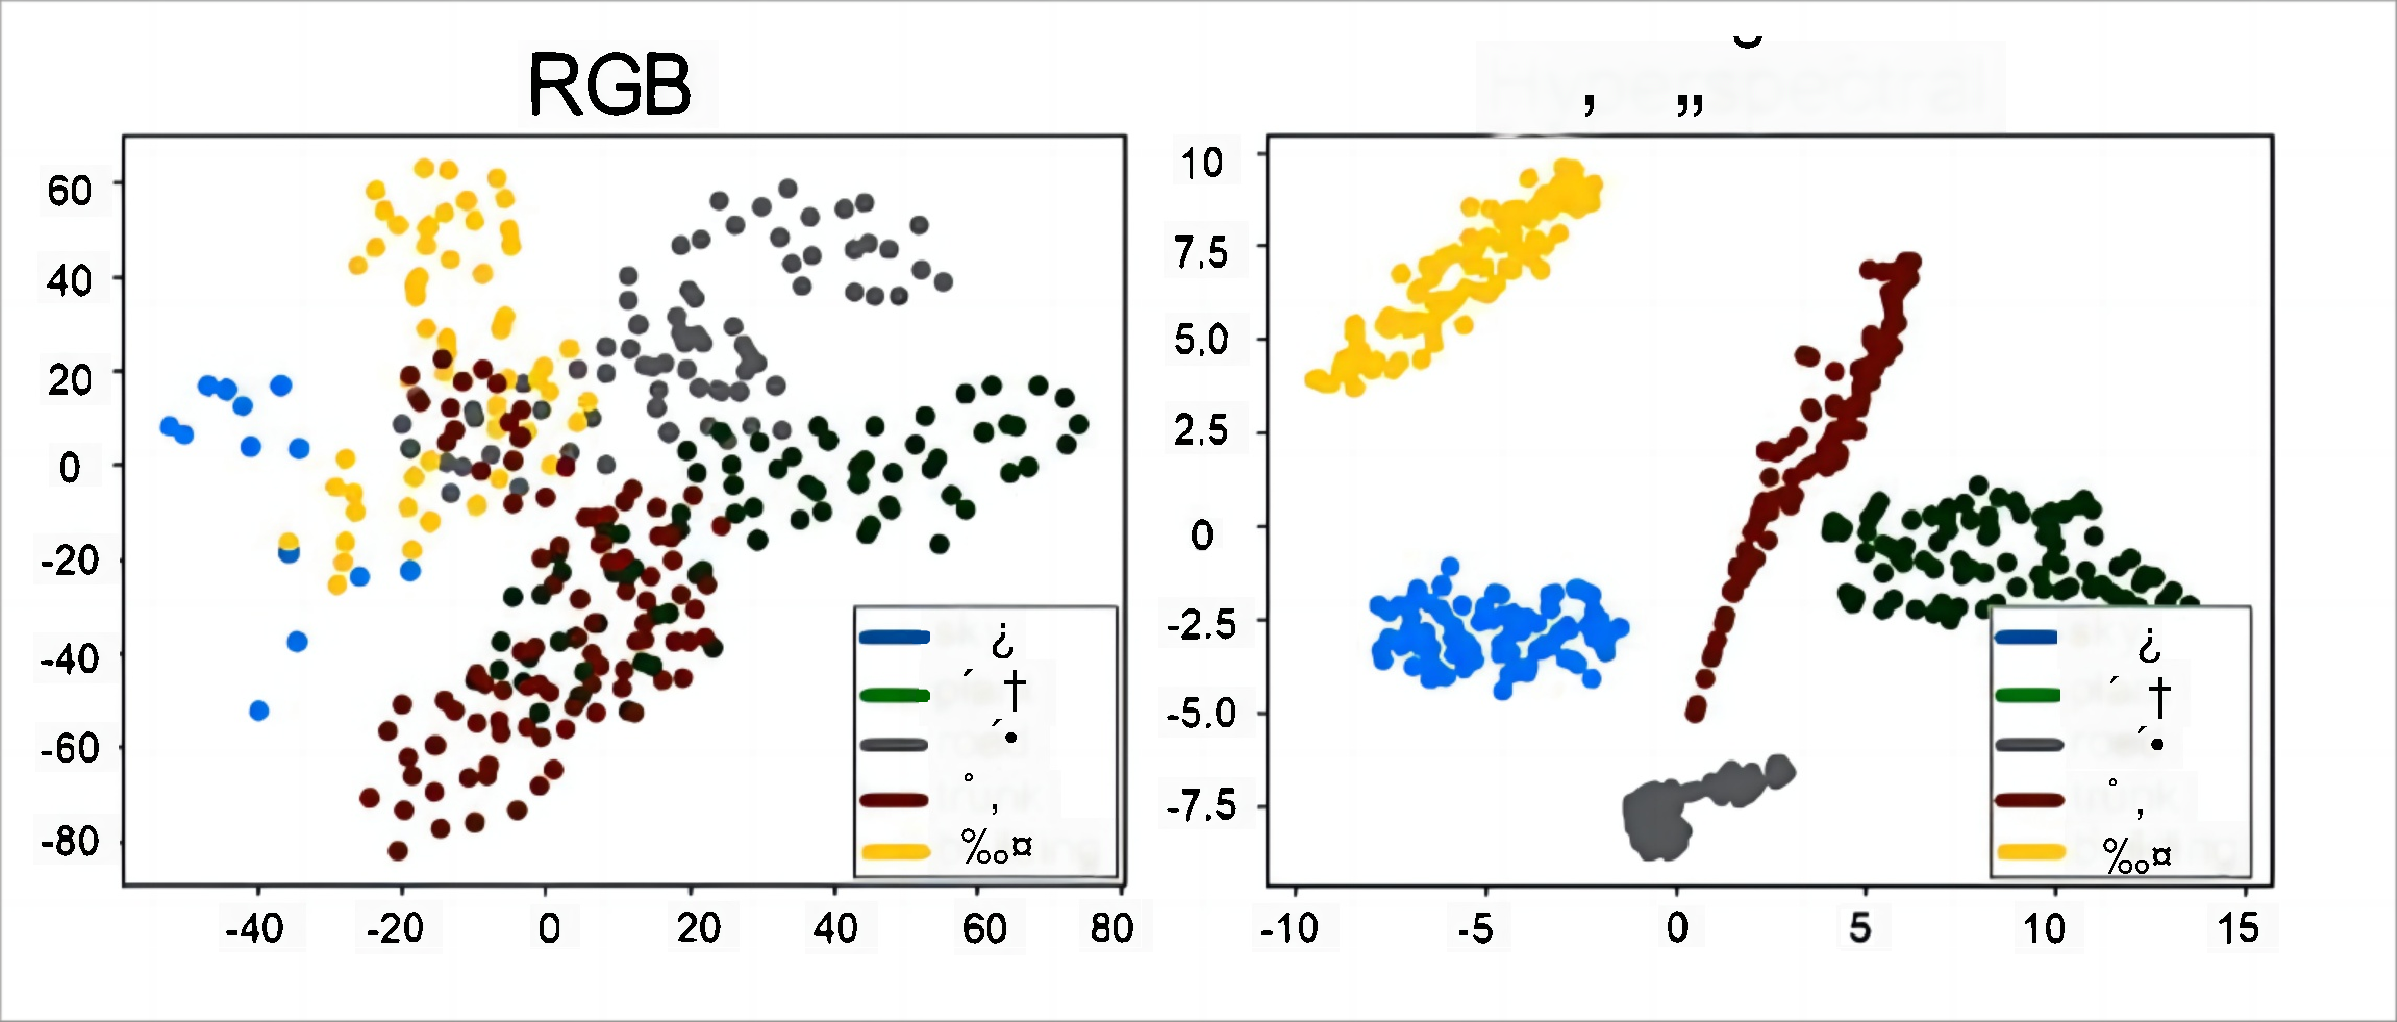
\includegraphics[width=1.0\linewidth]{docs/fig-chap4/fig-4-tsne.pdf}
% 	\caption{RGB域与高光谱域的t-SNE对比}
% 	\label{fig:seg tsne}
% \end{figure*}

为了将高光谱图像的反射率校正用在RGB图像上从而对RGB图像进行更准确的材质分割,本文使用光谱联合RGB分解模型,利用低空间分辨率光谱图像中的近红外和可见光波段辅助材质分割,低空间分辨率的光谱图像与高空间分辨率的RGB图像正好在光谱和空间两个维度上互补。

\begin{figure*}[h]
	\centering
	%\fbox{\rule{0pt}{2in} \rule{0.9\linewidth}{0pt}}
	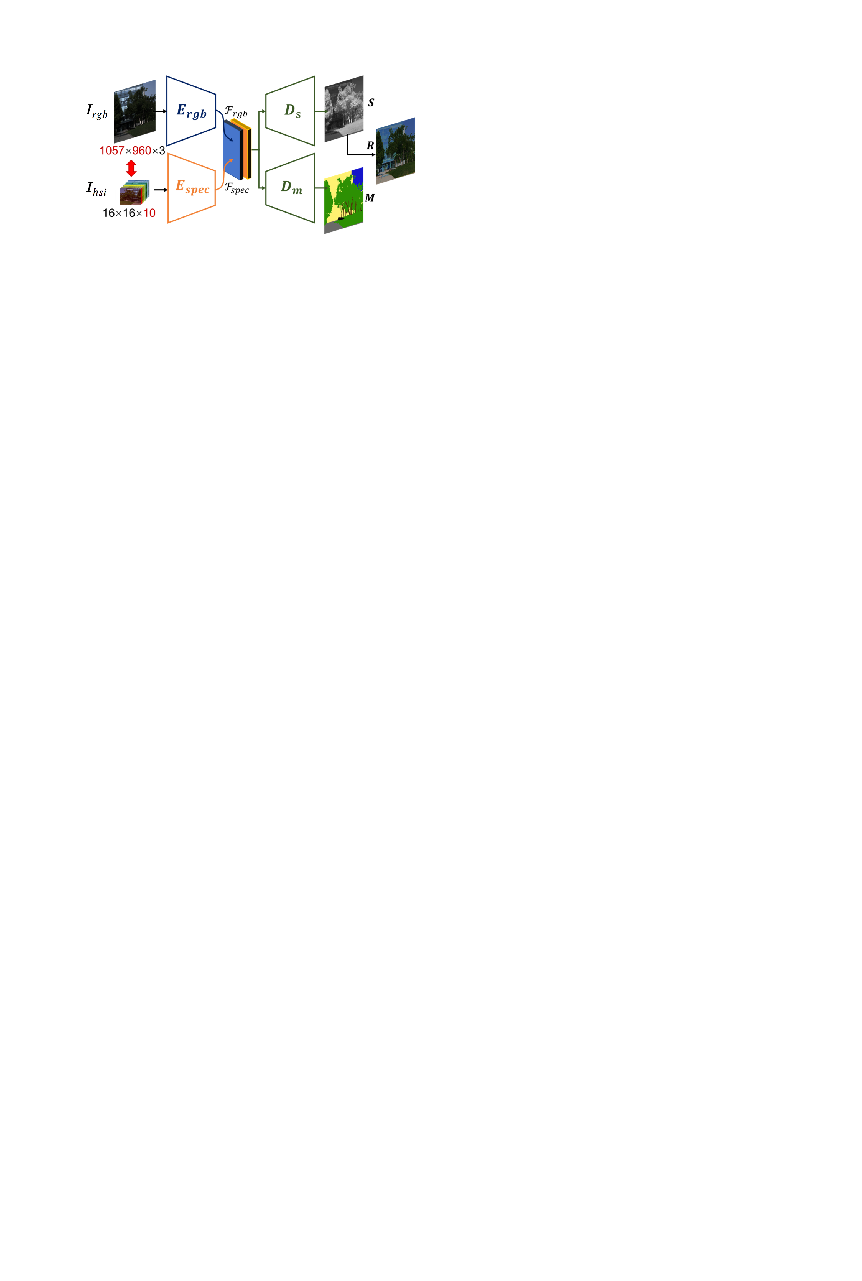
\includegraphics[width=1.0\linewidth]{docs/fig-chap4/fig-4-pipeline.pdf}
	\caption{光谱联合RGB分解模型示意图}
	\label{fig:seg pipeline}
\end{figure*}

如图\ref{fig:seg pipeline}所示,光谱联合RGB分解模型融合了两个独立的编码器和解码器,输入为高空间分辨率的RGB图像和低空间分辨率的光谱图像,输出为阴影图$S$和材质分割结果$M$,阴影图$S$可与光源光谱结合,进行反射率校正,得到反射率图$R$。

具体来说,将低空间分辨率光谱图像调整为与RGB图像相同的空间分辨率,并预训练RGB编码器$E_{rgb}$和光谱编码器$E_{spec}$,将RGB图像$I_{r g b}$和低空间分辨率光谱图像$I_{hsi}$投影到相同的隐空间进行特征的对齐,得到RGB图像的特征$\mathcal{F}_{r g b}$和高光谱图像的特征$\mathcal{F}_{spec}$:
\begin{equation}
\begin{align}
    \mathcal{F}_{rgb}=E_{rgb}\left(I_{rgb}\right),\\
    \mathcal{F}_{spec}=E_{spec}\left(I_{hsi}\right).
\end{align}
\end{equation}

然后通过串接操作将$\mathcal{F}_{r g b}$和$\mathcal{F}_{spec}$融合在一起,以共享互补的特征。

基于融合后的特征,利用解码器$D_{m}$和$D_{s}$独立预测材质分割$M$和阴影$S$。光谱联合RGB分解模型的解码器可以表示为:

\begin{equation}
M, S=D_{m,s}\left(\operatorname{concat}\left(\mathcal{F}_{r g b}, \mathcal{F}_{\text {spec }}\right)\right).
\end{equation}

分解得到的阴影$S$可以根据等式\ref{eq:reflectance}反过来对RGB图像进行反射率校正,并得到RGB图像的反射率图像$R$。

光谱联合RGB分解模型在训练时的损失函数包括材质分割相关的损失项和阴影图分解的损失项,表示为如下等式:

\begin{equation}
\ell  = \eta \ell_{mIoU}(M,M_{GT}) + (1-\eta) {\ell
_{L1}(S,S_{GT})}.
\end{equation}

其中$M$和$S$为预测的材质分割图和阴影图,$M_{GT}$和$S_{GT}$材质分割真值标注和阴影图真值,$\ell_{mIoU}$为平均交并比损失,$\ell
_{L1}$为L1损失,$\eta$为权重系数。当$\eta=1$时,光谱联合RGB分解模型可以看做纯材质分割模型;当$\eta=0$时,光谱联合RGB分解模型可以看做本征信息分解模型。
\begin{equation}
\begin{align}
\operatorname{IoU}_i(M,M_{GT}) &= \frac{|M(i) \cap M_{GT}(i)|}{|M(i) \cup M_{GT}(i)|},\\
\operatorname{mIoU}(M,M_{GT}) &= \frac{\sum_{i=0}^{n} 
 IoU_i(M,M_{GT})}{n+1},\\
    \ell_{mIoU}(M,M_{GT}) &= 1 - mIoU(M,M_{GT}).
\end{align}
\end{equation}

其中$n+1$表示材质分割的总类别数,$\operatorname{IoU}_i$表示第$i$类材质的交并比。

\begin{equation}
\ell_{L1}(S,S_{GT}) = | S - S_{GT}|.
\end{equation}



\section{实验过程与结果分析}
在本章研究中,实验设置所使用的硬件平台和相关软件同第二章实验设置部分。
\subsection{评价指标}
对于材质分割的结果,本文采用平均交并比(mean Intersection-over-Union,mIoU)作为评价指标对材质分割的准确度进行衡量。

如下等式定义了分割图A与分割图B的平均交并比:
% \begin{equation}
% \operatorname{IoU}(A, B)=\frac{|A \cap B|}{|A \cup B|}
% \end{equation}
\begin{equation}
\begin{align}
\operatorname{IoU}_i(A,B) &= \frac{|A(i) \cap B(i)|}{|A(i) \cup B(i)|},\\
\operatorname{mIoU}(A,B) &= \frac{\sum_{i=0}^{n} 
 IoU_i(A,B)}{n+1}.
\end{align}
\end{equation}

其中,$|X|$为集合$X$的大小,$\cap$和$\cup$分别为集合的交集和并集。将一张图像的每个像素(按照一定顺序)的标签视为一个元素,则每张图像中所有像素的标签代表一个有序集。预测的材质分割图与标注的材质分割图之间的mIoU越大,材质分割的准确度越高。由此,预测结果和人工标注可以使用mIoU度量进行比较。

\subsection{定性分析}

\begin{figure*}
	\centering
	%\fbox{\rule{0pt}{2in} \rule{0.9\linewidth}{0pt}}
	\includegraphics[width=1.0\linewidth]{docs/fig-chap4/fig-4-seg-result.pdf}
	\caption{材质分割结果图}
	\label{fig:seg result}
\end{figure*}

如图\ref{fig:seg result}所示,本文给出了在不同场景下的材质分割预测与人工标注的对比。

在第一行图像中,得益于阴影图的校正,阴影下的树干得到了较好的分割。在第二行图像和第五行图像中,分割失败的树干上同时有颜色的变化(白漆)和亮度的变化,即使进行了阴影图的校正仍未准确分割。在第二行图像和第三行图像中,同样得益于阴影图的校正,地面上的亮度变化并没有影响道路的分割。在第四行图像中,建筑的镂空部分原本应该是天空类,但本文提出的算法没能区分玻璃反射的天空与真实的天空,从场景图中可以看到天空与玻璃间有亮度的差异,但是本文使用阴影图进行校正后的反射率图(可参考图\ref{fig:enhance dataset})中天空和玻璃具有相似的亮度,仅从颜色上很难区分两者。

定性分析强调了使用阴影图进行反射率校正对材质分割的有效性。其优点在于减少了阴影变化对同一材质分割类别的整体一致性的影响,缺点在于使得原本需要用亮度进行区分的类别变得更难区分。


\subsection{定量分析}

在实际应用中,高光谱的波段数量和空间分辨率往往受到限制,因此有必要考量不同波段数量以及空间分辨率下的光源光谱辅助的效果。更少的波段数量和更低的空间分辨率通过从高空间分辨率的高光谱图像中下采样得到。


\begin{figure*}[h]
	\centering
	%\fbox{\rule{0pt}{2in} \rule{0.9\linewidth}{0pt}}
	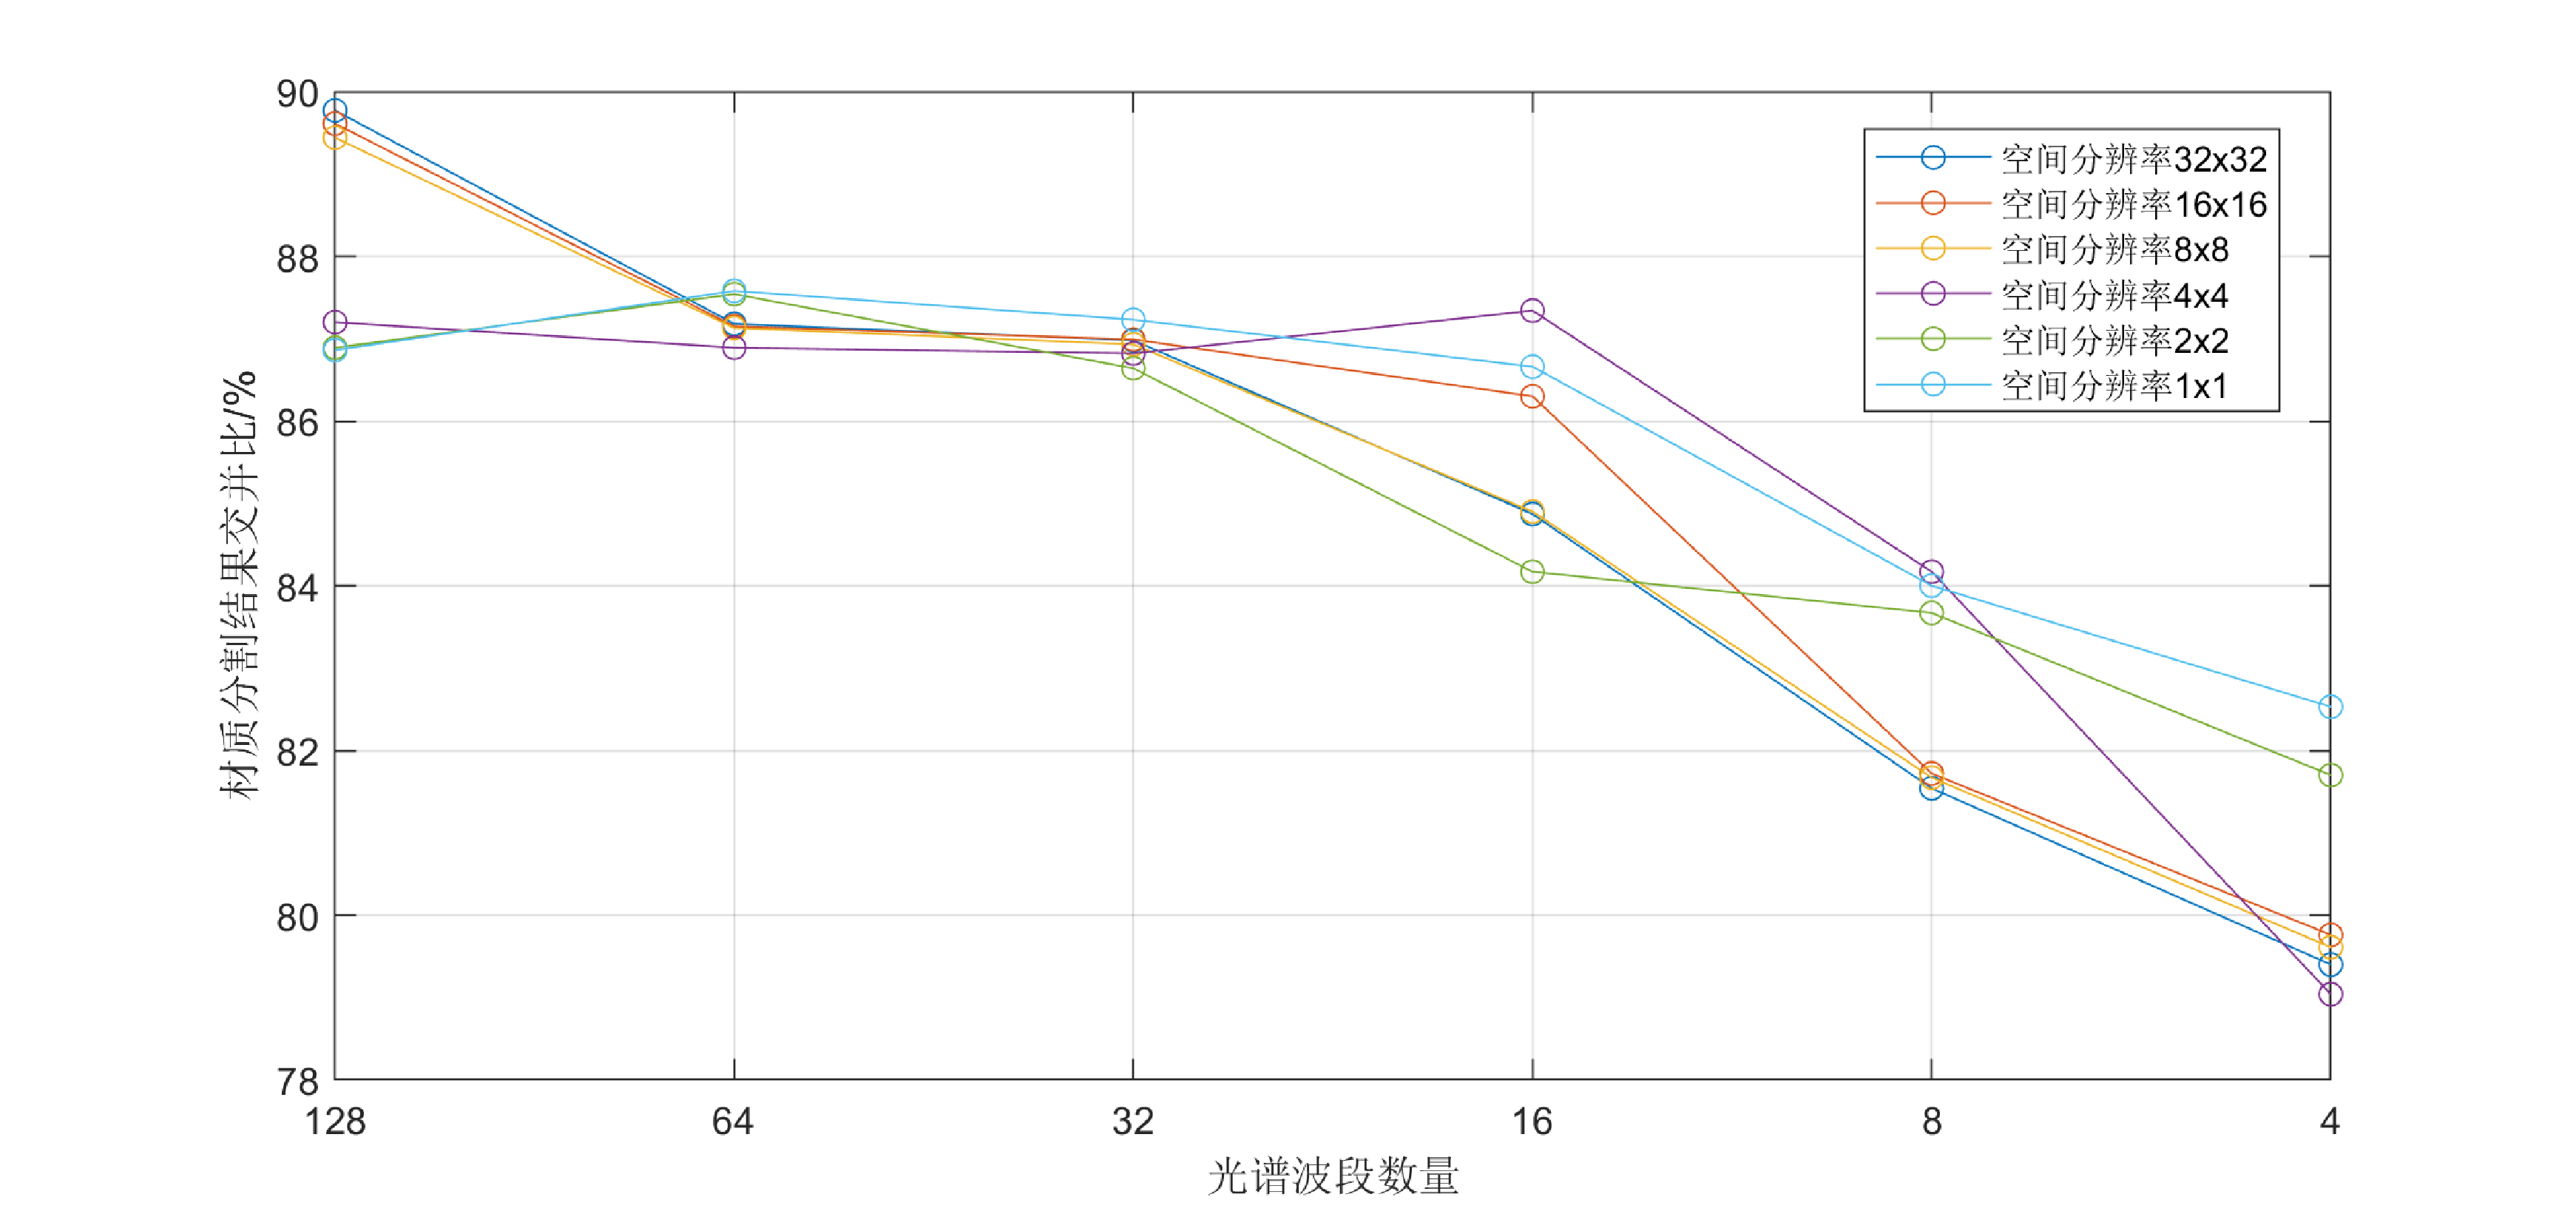
\includegraphics[width=1.0\linewidth]{docs/fig-chap4/fig-4-result-resolution.pdf}
	\caption{引入光源光谱波段数量以及空间分辨率对材质分割结果的影响}
	\label{fig:seg result resolution}
\end{figure*}


如图\ref{fig:seg result resolution}所示,随着光谱波段数量的降低,材质分割结果交并比总体上从90\%降低到了80\%,而引入的光源光谱的空间分辨率对材质分割结果的影响并不大。这或许是因为光源光谱是通过间接的方式辅助材质分割,网络中起主要作用的依然是高分辨率的RGB图像,但是光谱波段数量会影响反射率校正的精度,从而比较明显地影响RGB图像的分解以及材质分割。

由此可知,在该任务中,光谱波段数量的作用大于光谱空间分辨率的作用,这或许对于实际应用中光谱传感器的设计有一定的引导作用。


\begin{table}[h]
\caption{引入不同程度的光谱辅助下的材质分割交并比(\%)对比}
\label{tab:seg result}
\begin{tabular}{c|c|ccc|ccc|ccc}
\hline
通道选择     & 无     & \multicolumn{3}{c}{3通道RGB} & \multicolumn{3}{c}{16通道光谱} & \multicolumn{3}{c}{128通道光谱} \\ \hline
空间分辨率    & 无     & 1\times1     & 4\times4     & 16\times16  & 1\times1     & 4\times4     & 16\times16  & 1\times1     & 4\times4     & 16\times16   \\ \hline
天空      & 95.21 & 94.69   & 94.69   & 94.8   & 95.14   & 96.04   & 95.82  & 95.59   & 95.27   & \textbf{96.28}   \\
建筑 & 71.5  & 73.8    & 74.52   & \textbf{78.58}  & 78.46   & 76.92   & 77.34  & 77.79   & 77.91   & 76.79   \\
道路     & 53.16 & 67.41   & 78.39   & 76.15  & 77.86   & 84.69   & 82.09  & 75.1    & 80.04   & \textbf{86.71}   \\
绿植    & 88.14 & 90.98   & 93.11   & 92.86  & 92.81   & 94.06   & 93.87  & 92      & 93.62   & \textbf{94.51}   \\
树干    & 90.94 & 92.38   & 90.9    & 91.17  & 93.11   & 92.46   & 92.92  & 92.71   & \textbf{93.11}   & 92.2    \\ \hline
平均交并比    & 79.79 & 83.85   & 86.32   & 86.71  & 87.47   & 88.83   & 88.40  & 86.63   & 87.99   & \textbf{89.29}  \\ \hline
\end{tabular}
\end{table}

此外,不同类别的分割精度也呈现出很大差异,如表\ref{tab:seg result}所示,天空类别无需光谱辅助就能达到95\%左右的材质分割交并比;对于建筑类别,16\times16的空间分辨率的额外辅助的情况下,3通道RGB辅助的效果甚至可能优于更多通道的光源辅助的结果,分别为78.58\%和76.79\%;光谱辅助对道路类别的影响最大,在无辅助的情况下为53.16\%,在16\times16\times128的光谱的辅助下达到了86.71\%;对于绿植和树干类,引入额外的光谱辅助则有轻微的提升。

对于比较复杂的类别,例如建筑,光谱的引入几乎不起作用。这是因为建筑的复杂材质,如玻璃、砖块以及粉刷墙面的光谱反射率差别过大,反而在分割时起到反效果。而对于道路这类在RGB图像中色彩各异、在特定波段的光谱反射率却比较稳定的类别,则尤其适合用光谱辅助。


% \begin{figure*}[h]
% 	\centering
% 	%\fbox{\rule{0pt}{2in} \rule{0.9\linewidth}{0pt}}
% 	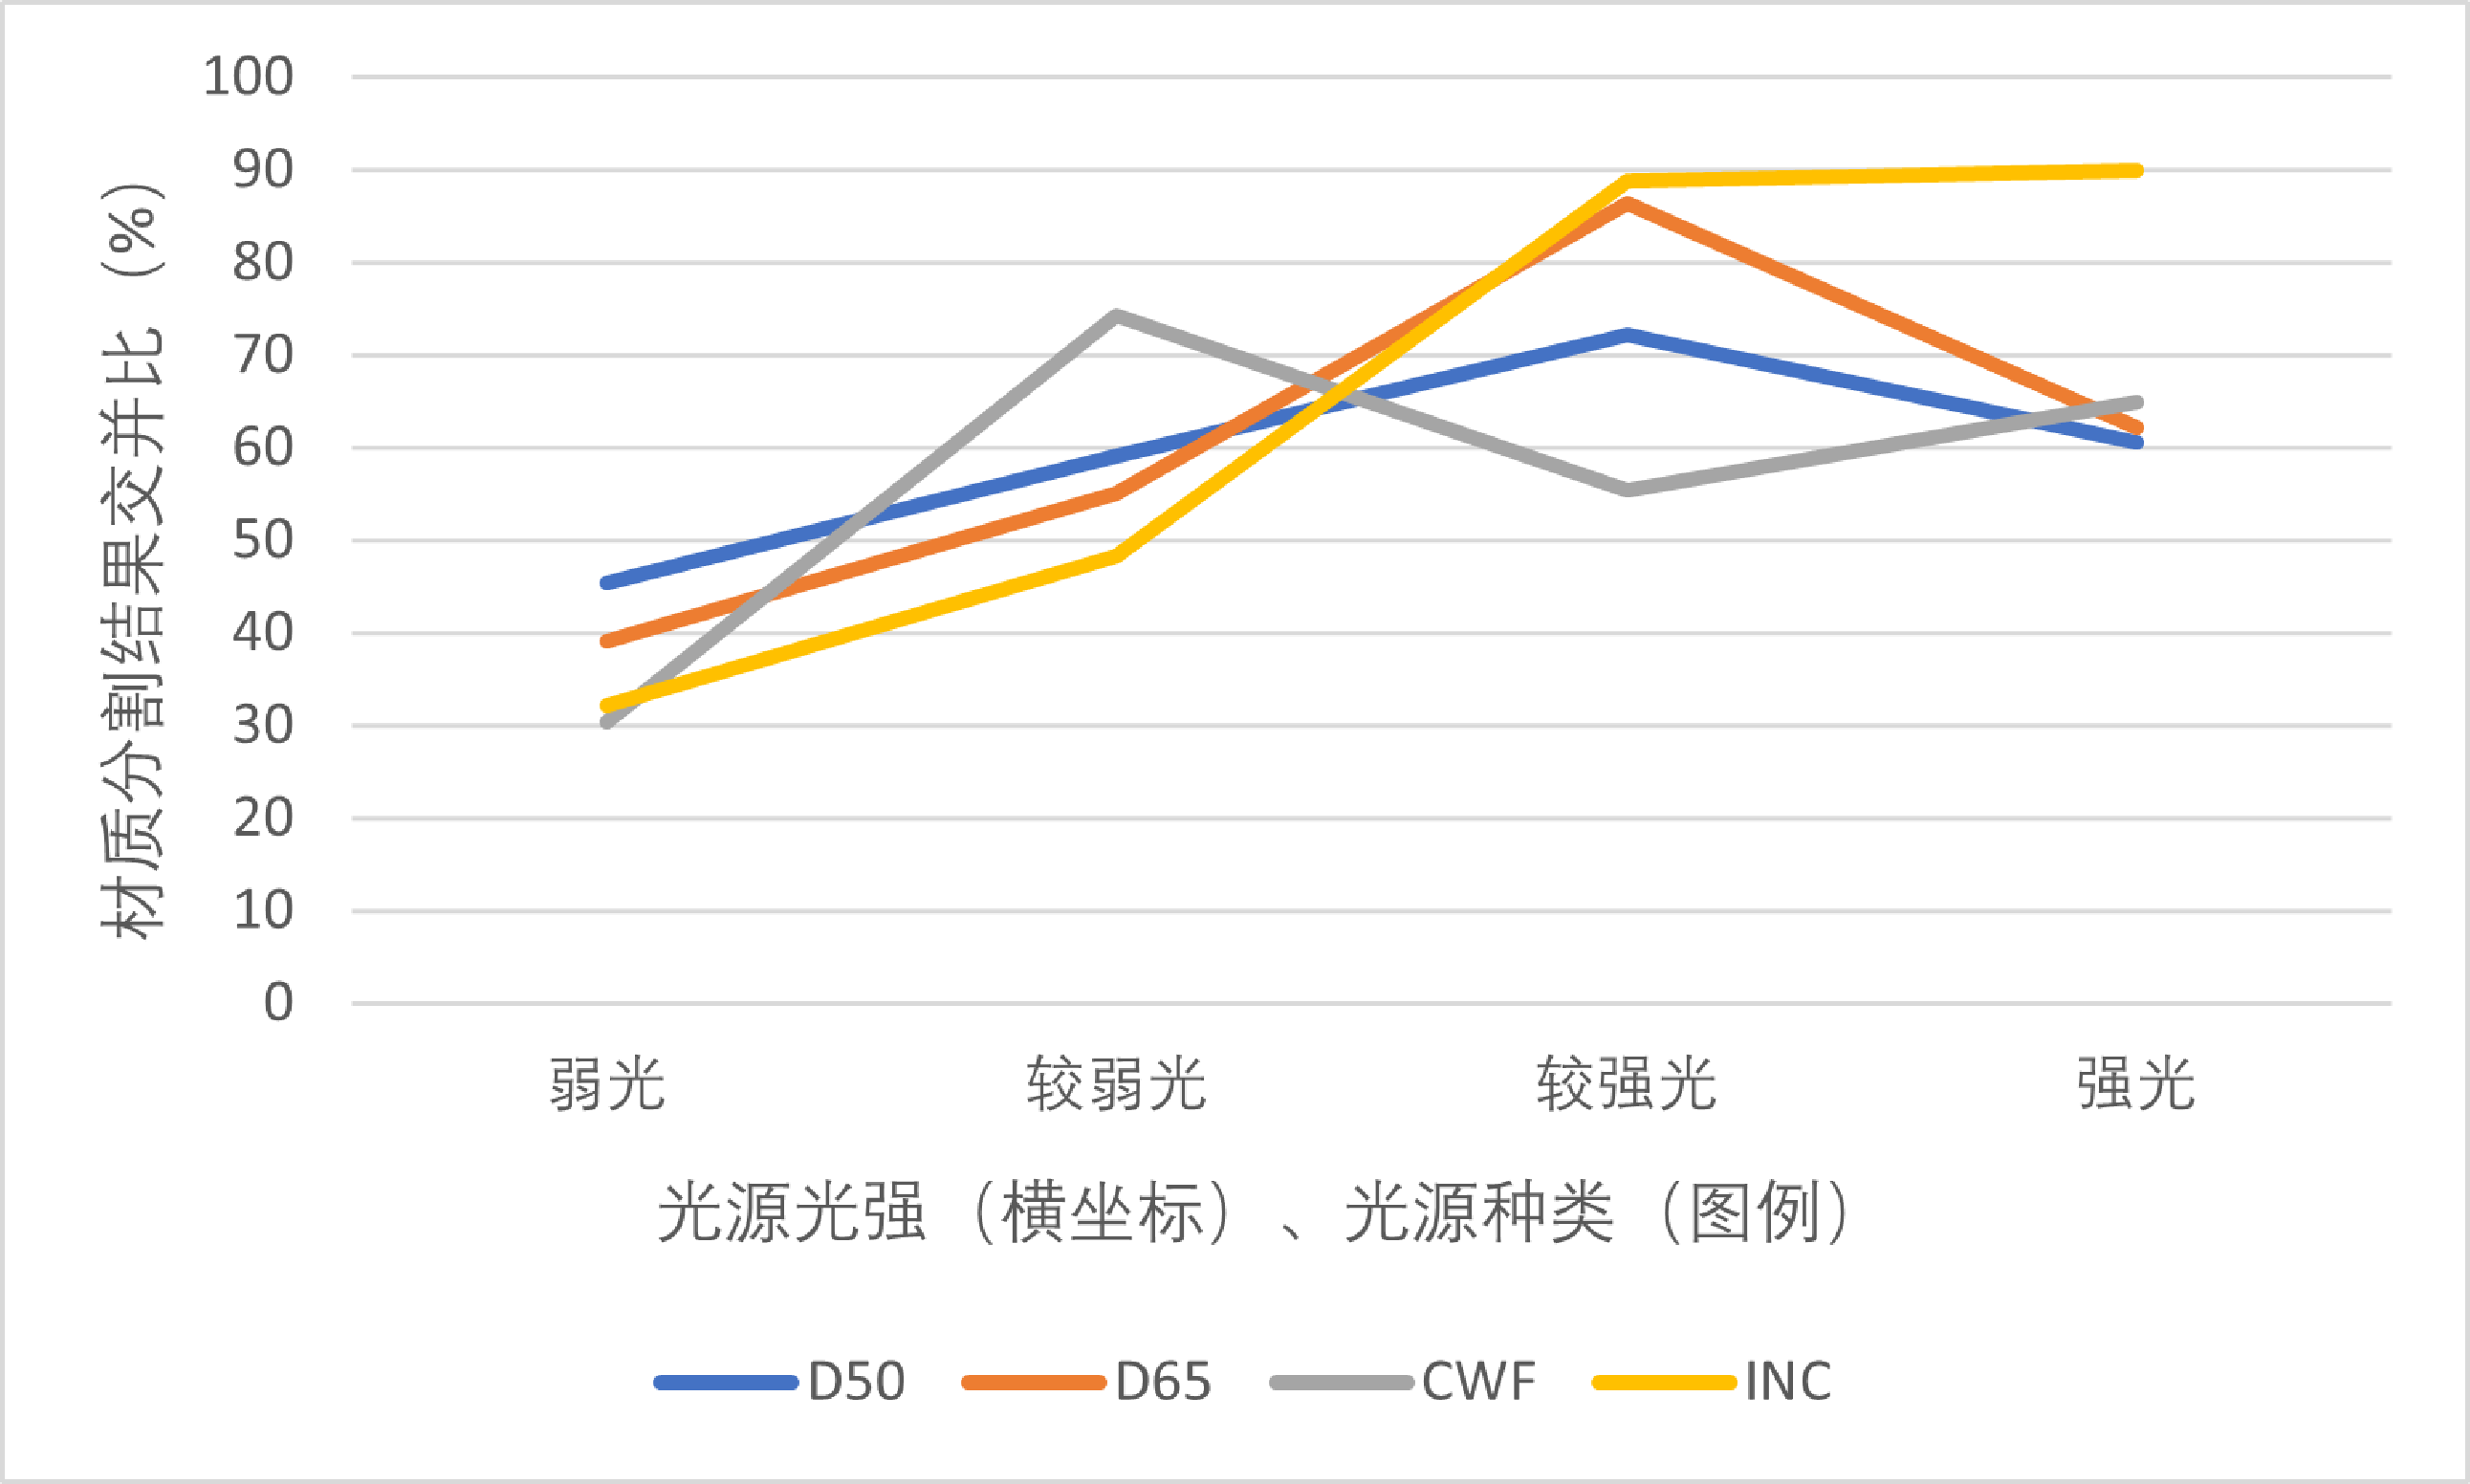
\includegraphics[width=1.0\linewidth]{docs/fig-chap4/fig-4-result-light.pdf}
% 	\caption{在不同光源种类以及亮度下的实验结果。}
% 	\label{fig:seg result light}
% \end{figure*}

\section{本章小结}
诸如材质分割等高层级的任务会受图像处理等低层级的任务的影响,在本章中,本文利用材质分割这个任务证明了光源校正的必要性和有效性,相较于未引入光源光谱校正的结果取得了明显的进步。这主要归功于本章方法在以下几个方面的研究:

1.通过将光源光谱作为材质分割网络的额外输入,提出了光谱联合RGB分解模型来利用光谱辅助RGB图像进行材质分割和阴影图预测,并推理反射率图。

2.利用光源光谱估计的结果来进行反射率校正,区分同样深色物体的反射率,从数据输入层面增加不同材质类别间的特征差异。

实验结果表明,更多的光源光谱波段、更高的空间分辨率的光谱辅助更有利于RGB的材质分割。本方法的不足之处在于目前尚无法完美解决“同物易谱”、“异物同谱”的问题,在反射率校正的精度方面仍有提升空间。
% ,而光源光谱来自于全局的估计,因此对光源光谱估计的准确度有很高要求。

% %-------------------------------------------------------------------
%	第五章
%---------------------------------------------------------------------
\chapter{总结与展望}
\section{总结}
% 光谱反射率是材质固有的物理特性,广泛应用于各种视觉任务中,如环境、农业、地质和矿产勘探、生物、医学和军事等。然而,获取精确的光谱反射率图像需要对每幅图像进行额外的校准,来去除不同光源的影响,例如在场景中放置漫反射板。为了更方便
本文围绕高光谱图像的光源光谱估计问题及其应用展开研究。总体可以分为三个部分:其一是高光谱图像的光源光谱估计任务本身,对给定的高光谱图像预测其光源光谱;其二是光源光谱引导的图像增强,使用光源光谱引导高动态范围RGB图像的增强;其三是光源光谱校正的材质分割,使用光源光谱进行反射率校正并辅助RGB图像的材质分割。具体工作如下:

% 在本章节,我们提出了一种端到端网络来解决高光谱光源估计问题。 我们的方法使用更深的主干网络,引入通道和空间自注意以及平滑损失,并且显着优于以前的方法。 该方法在合成图像和真实图像上的良好性能显示了其有效性、灵活性和泛化能力。 我们构建了一个具有不同光源的真实高光谱图像的大型数据集进行测试,可以将其用于未来的训练和分析工作。 我们希望我们提出的无白板光源校准方法能够将现有的未校正的高光谱数据集纠正为准确的高光谱反射率数据集,并更好地用于高层级任务。并对镜面反射分解和深度展开网络进行介绍,
一、归纳并探讨现有的光源估计算法,分析了基于统计和基于学习的光源估计算法的优劣,在此基础上,本文构建了真实而非仿真的高光谱光源估计数据集并对算法进行了改进。本文提出了光谱联合空间自注意机制,在增强了特征图对特定通道和位置信息的感知的同时,有效缓解了基于学习的光源光谱估计任务中高光谱数据计算量大、网络参数多、训练慢的问题。此外,将损失函数改进为平滑约束的损失函数,有效避免了不实际的病态结果,从而提升了光源估计的准确度。

% 先前的方法在学习HDR场景下准确的色调增强方面面临挑战,而我们的先验引导的JDM-HDRNet通过有效地利用光谱联合RGB联合分解模型预测的S、R先验来提供明确的指导,从而优于先前的方法。,分析了用于RGB图像色调映射的三维查找表和HDRNet
二、在预测出高光谱图像的光源光谱的基础上,本文探索其对RGB图像增强的作用。构建了高动态范围RGB图像与高光谱图像对齐的图像增强数据集。在此基础上,提出了局部亮度适应法,在室外太阳光下使用近红外光源光谱修正RGB图像的局部亮度,为16位源图动态范围压缩到8位目标图提供了有效的预处理。另外,将低空间分辨率的光谱图像作为RGB图像增强的第二路输入,提出了光谱感知自注意机制,将光谱特征嵌入到RGB特征图中,从而提升了RGB图像增强的效果。

% 诸如材质分割等高层级的任务会受图像处理等低层级的任务的影响,在本章我们利用材质分割这个任务证明了光源校正的有效性,并提出了RGB-光谱联合分解模型来进一步利用光谱辅助RGB图像进行材质分割。实验结果表明更多的光源光谱波段、更高的空间分辨率的光谱辅助更有利于RGB的材质分割,而光源光谱来自于全局的估计,因此对光源光谱估计的准确度有很高要求。介绍了基于Transformer的语义分割方法,
三、在将光源光谱应用于低层级任务的基础上,本文进一步探索其在高层级任务的作用。本文提出的高光谱材质分割数据集可以为进一步的材质分割提供精确的反射率。基于本文上述的光源光谱估计算法,对用于材质分割的图像进行反射率校正预处理,在此基础上,将低空间分辨率的光谱反射率图像与高空间分辨率的RGB图像使用光谱联合RGB分解模型联合分解,提高了RGB图像的材质分割精度。

\section{展望}
目前,高光谱成像在民用和工业界应用还不够广泛,技术尚不够成熟。现有的高光谱成像系统还难以嵌入到小型的、轻便的或手持的移动端设备中,且高维度数据的计算受制于有限的算力。在未来,高维视觉信息的感知与计算会越来越普遍,相应的算法也会与时俱进。同时,因个人的眼界、学识和研究时间等方面的限制,本论文尚存在一些不足之处,有待于在今后研究工作中进
一步完善。下面对本文涉及的研究方向进行展望:

% 一、受制于实验条件,本文的高光谱图像光源光谱数据集是在单一的打光方向拍摄的,光场光谱研究同时也会将光源光谱的研究提升到更高维度的光源光场光谱研究,这对未来的光谱估计又是新的挑战。

一、在光源校正流程高度自动化,高光谱采集设备的使用普及化以及高维数据的传输便捷化后,通用的大规模高光谱图像数据集将会逐渐被构建,并应用于各种高光谱图像相关任务的预训练。

二、本文用于RGB图像增强的低空间分辨率光谱图像的空间分辨率建议至少为16\times 16,这在目前的智能手机上尚未实现。随着未来光谱成像元件与系统的小型化、集成化的发展,有望在小型的、轻便的或手持的移动端实现高分辨率的光谱成像,从而将实验中的更高分辨率下的结果转化为现实应用。

三、光源光谱校正的材质分割在未来可能应用于自动驾驶,考虑到驾驶过程中环境光的差异,仿照人眼的自适应性,合适的光源校正或许更有利于视觉模型的认知。

% 本研究中低空间分辨率光谱图像的空间分辨率固定为16\times16,这在商用高端智能手机上还无法实现。提高空间分辨率将提高联合分解模型中阴影和物质先验的预测精度。在移动设备上的图像增强和相关应用的背景下,需要进一步探索解决受限的光谱成像能力。
%---------------------------------------------------------------------
%	参考文献
%---------------------------------------------------------------------
% \newpage
% \phantomsection
% \addcontentsline{toc}{section}{参考文献}
% \begin{thebibliography}{99}
% \end{thebibliography}

% \clearpage
% %\setcounter{secnumdepth}{0}
% \ctexset{section/numbering=false}
% \section{致谢}
% %\addcontentsline{toc}{section}{致谢}
% \bibliographystyle{IEEEtran}
% \clearpage
% \phantomsection
% \addcontentsline{toc}{chapter}{参考文献} %向目录中添加条目,以章的名义
% \bibliography{njuthesis-sample.bib}

% 生成参考文献页

\printbibliography[heading=bibintoc, title=参考文献]

%---------------------------------------------------------------------
%	致谢
%---------------------------------------------------------------------

\begin{acknowledgement}

回首三年的硕士研究生生涯,非常感谢在我身边默默关注、支持我的老师、同学和父母,优秀的你们给我做出了最好的榜样,激励着我朝更高、更远的目标前进。  

感谢我的导师曹汛教授,曹老师学识渊博、工作严谨,是我引以为豪的导师和榜样。曹老师不但指导和帮助我进行科学研究、论文写作,而且在平时的学习和生活中对我悉心教导,关怀有加。曹老师给予了我很多学术指导以及丰富的科研资源,带领我们一众研究生参加杭州、天津等地的学术会议,开阔了我的学术视野,坚定了我继续从事学术研究的信心。衷心感谢曹汛老师三年来对我的关心和指导!

感谢沈秋副教授,沈老师拓宽了我的研究课题,在我的科研过程中给出了许多宝贵的意见和建议。沈老师在帮助我修改专利和论文的过程中,表现出敏锐的科研洞察力和精益求精的学术精神,让我对科研有了更深的理解。

感谢南京大学计算成像实验室(CITE Lab)的师兄:陈林森、字崇德、邓智威、黄尔齐、李昀谦、祖永祥、周凯来、蔡李靖、庄义昱、金周宇等。尤其感谢周凯来师兄引领我发表国际顶会论文、参与全国性竞赛,让我领会了要注重学术研究和科研活动过程中的每一步细节。

感谢和我同级进入CITE Lab实验室的同学以及陆续到来的学弟学妹:吕涛、施展、孙旭森、吴萌华、袁庆博、刁政宇、叶浩、杨富强、徐志成、董祥宇、张梦雅、黄成龙、胡李豪、李世桥、李齐平、张丁源等。感谢你们和我一同融入实验室,尤其感谢吕涛、施展和叶浩,我们共同进行学术研究和讨论,我们一起泛舟湖上的快乐时光是我宝贵的记忆。

感谢我的父亲和母亲,是他们让我无后顾之忧地投入学习与学术研究,探索人生与科研的乐趣,让我拥抱世界、走向未来。

 \rightline{王乙卜}
 \rightline{2024年5月于南京大学}
\end{acknowledgement}


\njuchapter{攻读硕士学位期间研究成果}
[1]	T Lv, H Ye, Q Yuan, Z Shi, \textbf{Y Wang}, S Wang, X Cao, “Aperture Diffraction for Compact Snapshot Spectral Imaging”. IEEE/CVF International Conference on Computer Vision (ICCV), 2023.

[2]	Z Shi, H Ye, T Lv, \textbf{Y Wang}, X Cao, “Compact Self-adaptive Coding for Spectral Compressive Sensing”. IEEE International Conference on Computational Photography (ICCP), 2023.

[3]	K Zhou, \textbf{Y Wang}, T Lv, Y Li, L Chen, Q Shen, X Cao, “Explore Spatio-temporal Aggregation for 
Insubstantial Object Detection: Benchmark Dataset andBaseline”. IEEE/CVF Conference on Computer Vision and Pattern Recognition (CVPR), 2022.

[4]	\textbf{王乙卜},沈秋,曹汛。一种基于高光谱的自动驾驶场景分割方法,中国发明专利,已公开,公开号:CN115661818A

% [5]	周凯来,\textbf{王乙卜},吕涛,陈林森,字崇德。视频级目标检测模型的训练方法及装置、设备、存储介质,中国发明专利,CN114419520A

[5]\textbf{王乙卜},杨富强,徐志成。MBIST自动规划分组算法,第五届集成电路EDA设计精英挑战赛三等奖,2023

[6]吕涛,施展,\textbf{王乙卜},霍城城,叶浩,徐志成,董祥宇,俞瀚洋,王琳翔,黄尔齐,周凯来,指导教师\ 曹汛,沈秋。基于国产解决方案的天然气管道沿线危险目标检测关键技术与工业化实践,第九届中国国际大学生创新大赛金奖,2023

[7]吕涛,\textbf{王乙卜},施展,周凯来,指导教师\ 曹汛。化工气体泄漏光谱视频智能检测算法,第三届中国研究生人工智能创新大赛一等奖,2021

% \njupaperlist[攻读硕士学位期间发表的专利]
% \njupaperlist[攻读硕士学位期间发表的学术论文]
% {zhou2022explore,lv2023aperture,shi2023compact
% }

%---------------------------------------------------------------------
%	附录部分
%---------------------------------------------------------------------

% 附录部分使用单独的字母序号
% \appendix

% 可以在这里插入补充材质

% 完工
\end{document}
